\chapter{Geodesics in Kerr spacetime: generic and timelike cases}
\label{s:gek}
\index{geodesic!in Kerr spacetime}

\minitoc

\section{Introduction}

\section{Equations of geodesic motion}

\subsection{Introduction} \label{s:gek:geod_motion_intro}

In all this chapter, we are concerned with the motion of a particle
$\mathscr{P}$ in the Kerr spacetime $(\M,\w{g})$, under the hypothesis that $\mathscr{P}$
feels only gravity, as described by $\w{g}$ (freely falling particle).
The worldline $\Li$ of $\mathscr{P}$
is then necessarily a geodesic\footnote{The definition and basic properties of geodesics
are recalled in Appendix~\ref{s:geo}; see also Sec.~\ref{s:fra:geod_motion}.} of
$(\M,\w{g})$. It is a timelike geodesic if $\mathscr{P}$ is a massive particle
and a null geodesic if $\mathscr{P}$ is massless (e.g. a photon).

In a given coordinate system $(x^\alpha)$, the geodesic $\Li$ is described
by a system of the form\footnote{In Appendices~\ref{s:bas} and \ref{s:geo},
a different symbol is used for the function $X^\alpha(\lambda)$ defining
$\Li$ and the coordinate $x^\alpha$ (cf. Secs.~\ref{s:bas:vectors} and
\ref{s:geo:geodesic_eq}). Following standard usage in the physics literature,
we shall not do this in this chapter.}
$x^\alpha = x^\alpha(\lambda)$, where $\lambda$ is an
affine parameter\footnote{See Sec.~\ref{s:geo:def} for the definition
of an affine parameter along a geodesic.} along $\Li$. We choose $\lambda$ to be the affine parameter
associated with $\mathscr{P}$'s 4-momentum $\w{p}$,
i.e. such that $\D x^\alpha / \D\lambda = p^\alpha$ [Eq.~(\ref{e:fra:p_dxdl})].
In particular, $\lambda$ is dimensionless and is increasing towards the future\footnote{Let us recall that the Kerr spacetime is time-oriented, cf. Sec.~\ref{s:ker:time_orientation}.} along $\Li$.
The curve $\Li$ is a geodesic iff the functions $x^\alpha(\lambda)$ obey
the geodesic equation [Eq.~(\ref{e:geo:eq_geod}) in Appendix~\ref{s:geo}]:
\be \label{e:gek:eq_geod}
    \frac{\D^2 x^\alpha}{\D\lambda^2} + \Gamma^\alpha_{\ \, \mu \nu}
    \frac{\D x^\mu}{\D\lambda} \frac{\D x^\nu}{\D\lambda} = 0 ,\qquad 0 \leq \alpha \leq 3,
\ee
where the $\Gamma^\alpha_{\ \, \mu \nu}$'s are the Christoffel symbols\index{Christoffel symbols} of the metric $\w{g}$
with respect to the coordinates $(x^\alpha)$, as given by Eq.~(\ref{e:bas:Christoffel}).
Equation~(\ref{e:gek:eq_geod}) is the component expression of
$\wnab_{\w{p}} \, \w{p} = 0$ [Eq.~(\ref{e:fra:p_geodesic})]. It is
a system of four coupled second-order
differential equations, which are non-linear. We are going to see that it is actually not necessary to
solve this system to compute the geodesics of Kerr spacetime. Indeed,
as in the Schwarzschild case studied in Chap.~\ref{s:ges}, there exists
enough first integrals of Eq.~(\ref{e:gek:eq_geod}) to reduce
the problem to four first-order equations
of the type $\D x^\alpha/\D\lambda = F^\alpha(x^0, x^1, x^2, x^3)$.

Three integrals of motion are similar to those of Schwarzschild geodesics:
one is the particle's mass $\mu$ (Sec.~\ref{s:gek:mass_int_motion} below)
and the two other ones are
the conserved energy $E$ and the conserved angular momentum
$L$ (Sec.~\ref{s:gek:int_motion_sym}), which arise from the common symmetries
of Kerr and Schwarzschild spacetimes: stationarity (outside the ergoregion) and axisymmetry.
In the Schwarzschild case, the fourth integral of motion was provided by
spherical symmetry, which constrained all geodesics to be planar, so that
a suitable choice of
coordinates $(t,r,\th,\ph)$ makes a given geodesic confined to the
hyperplane $\th=\pi/2$, yielding the first integral $p^\th=0$ [Eq.~(\ref{e:ges:pth_zero})].
The Kerr spacetime with $a\not=0$ being not spherically symmetric, we loose
this property here. Fortunately there exists another
integral of motion, known as the \emph{Carter constant}; it arises from a remarkable property
of Kerr spacetime: the existence of a non-trivial Killing tensor (Sec.~\ref{s:gek:Carter_const}).
This makes a total of four integral of motions,
which makes the problem integrable (Secs.~\ref{s:gek:first_order_system} to
\ref{e:gek:integration}).


\subsection{Integrals of motion from spacetime symmetries} \label{s:gek:int_motion_sym}

As for Schwarzschild spacetime (cf. Sec.~\ref{s:ges:fiom}), we have the following
property.
\begin{greybox}
The Killing vectors $\w{\xi}$ and $\w{\eta}$ of Kerr spacetime,
associated respectively with
stationarity and axisymmetry [cf. Eq.~(\ref{e:ker:def_xi_eta})],
give birth to two conserved quantities
along any geodesic $\Li$:
\begin{subequations}
\label{e:gek:def_E_L}
\begin{align}
& \encadre{E := - \w{\xi}\cdot \w{p} = - \w{g}(\w{\xi},\w{p}) } \label{e:gek:def_E} \\
& \encadre{L := \w{\eta}\cdot \w{p} = \w{g}(\w{\eta},\w{p}) } , \label{e:gek:def_L}
\end{align}
\end{subequations}
where $\w{p}$ is the 4-momentum of the particle $\mathscr{P}$
having $\Li$ as worldline (cf. Sec.~\ref{s:fra:worldlines}).
For the same reasons as in Sec.~\ref{s:ges:fiom}, $E$ is called
the \defin{conserved energy}\index{conserved!energy}\index{energy!conserved --}
or \defin{energy at infinity}\index{energy!at infinity} of $\mathscr{P}$,
while $L$ is called the \defin{conserved angular momentum}\index{conserved!angular momentum}\index{angular momentum!conserved --}
or \defin{angular momentum at infinity}\index{angular momentum!at infinity}
of $\mathscr{P}$.
\end{greybox}
In particular, if $\Li$ reaches the asymptotic region $|r|\to+\infty$,
$E$ is nothing but $\mathscr{P}$'s energy as measured by the asymptotic inertial
observer introduced in Sec.~\ref{s:ker:asymp_inertial_obs}, given that
the 4-velocity of the latter coincides with the Killing vector
$\w{\xi}$
[compare Eq.~(\ref{e:fra:E_obs}) with Eq.~(\ref{e:gek:def_E})].
Similarly, $L$ is the component along the rotation axis of $\mathscr{P}$'s (total) angular momentum vector $\w{L}_{\rm tot}$
as measured by the asymptotic inertial observer.

\begin{remark}
Because it represents only a component of the total angular momentum,
$L$ is sometimes denoted by $L_z$.
\end{remark}

In coordinates $(t,r,\th,\ph)$ adapted to spacetime symmetries,
i.e. coordinates such that $\w{\xi} = \wpar_t$ and $\w{\eta}=\wpar_\ph$,
for instance Boyer-Lindquist coordinates (Sec.~\ref{s:ker:expr_BL}),
Kerr coordinates (Sec.~\ref{s:ker:Kerr_coord}) or 3+1 Kerr coordinates
(Sec.~\ref{s:ker:3p1_Kerr_coord}), one can rewrite
(\ref{e:gek:def_E_L})
in terms of the components $p_t = g_{t\mu} \, p^\mu$ and $p_\ph = g_{\ph\mu} \, p^\mu$
of the 1-form $\uu{p}$ associated to $\w{p}$ by metric duality:
\begin{subequations}
\label{e:gek:E_pt_L_pph}
\begin{align}
& E = - p_t \\
& L = p_\ph
\end{align}
\end{subequations}
Indeed, in such a coordinate system, $\xi^\mu =  \delta^\mu_{\ \, t}$
and $\eta^\mu = \delta^\mu_{\ \, \ph}$, so that $E = -g_{\mu\nu} \, \xi^\mu p^\nu = -g_{t\nu} \, p^\nu = -p_t$
and $L = g_{\mu\nu} \, \eta^\mu p^\nu = g_{\ph\nu} \, p^\nu = p_\ph$.

\begin{example}[Generators of the event and inner horizons] \label{x:gek:null_generator_hor}
Let us choose for $\Li$ a null geodesic generator of the event horizon $\Hor$
(cf. Sec.~\ref{s:gek:null_gen_hor}). $\Li$ is then an outgoing principal null
geodesic and the 4-momentum vector $\w{p}$ is proportional to the null vector
$\wl \equalH \w{\chi} = \w{\xi} + \Omega_H \w{\eta}$ [Eq.~(\ref{e:ker:l_eqH_chi})
and (\ref{e:ker:def_chi})].
By definition of a
generator of a null hypersurface (cf. Sec.~\ref{s:def:null_geod_gen}),
$\w{p}$ is normal to $\Hor$. Since the Killing vector fields $\w{\xi}$ and $\w{\eta}$
are tangent to $\Hor$ (for $\Hor$ is globally preserved by the
spacetime symmetries), we get immediately from
the definitions (\ref{e:gek:def_E_L}) $E=0$ and $L=0$.
Similarly, if $\Li$ is a null geodesic generator of the
inner horizon $\Hor_{\rm in}$, $\Li$ is an outgoing principal null
geodesic, with $\w{p}$ proportional to
the null normal
$\wl \stackrel{\Hor_{\rm in}}{=} \w{\chi}_{\rm in} = \w{\xi} + \Omega_{\rm in} \w{\eta}$
[Eq.~(\ref{e:ker:chi_in_ell}) and (\ref{e:ker:def_chi_in})], so that we
have $E=0$ and $L=0$ as well. Hence we conclude:
\be \label{e:gek:generator_hor_E_L_zero}
    \Li \ \mbox{null geodesic generator of}\ \Hor\ \mbox{or}\ \Hor_{\rm in}
   \  \Longrightarrow\  E = 0 \quad\mbox{and}\quad L = 0 .
\ee
\end{example}

\begin{example}[Ingoing principal null geodesics] \label{x:gek:ingoing_null_E_L}
For the ingoing principal null geodesics $\Li^{\rm in}_{(v,\th,\tph)}$
introduced in Sec.~\ref{s:ker:principal_geod}, the 4-momentum vector
is
\be \label{e:gek:p_alpha_k}
    \w{p} = \alpha \w{k} ,
\ee
where $\alpha$ is a (positive) constant, since $\w{k}$ is a geodesic vector
[Eq.~(\ref{e:ker:nab_k_k})], as $\w{p}$ [Eq.~(\ref{e:fra:p_geodesic})].
Equations~(\ref{e:gek:E_pt_L_pph}) with the components relative to the 3+1 Kerr coordinates
$(\ti, r, \th, \tph)$ lead then to
\[
    E = - \alpha k_{\ti} = - \alpha(-1) = \alpha \qand
   L = \alpha k_{\tph} = \alpha a \sin^2\th,
\]
where the components $k_{\ti}$ and $k_{\tph}$
have been read on Eq.~(\ref{e:ker:k_form_Kerr}).
Hence for any ingoing principal null geodesic $\Li^{\rm in}_{(v,\th,\tph)}$,
\be \label{e:gek:ingoing_null_E_L}
    E > 0 \qand L = a E \sin^2 \th .
\ee
Recall that $\th$ is constant along $\Li^{\rm in}_{(v,\th,\tph)}$, so that
the above formula does yield a constant value for $L$. Moreover, it fulfills
$L\geq 0$ with $L=0$ only for $a=0$ or $\th\in\{0,\pi\}$ (rotation axis).
\end{example}

\begin{example}[Outgoing principal null geodesics] \label{x:gek:outgoing_null_E_L}
For the outgoing principal null geodesics $\Li^{\rm out}_{(u,\th,\tilde{\tph})}$
introduced in Sec.~\ref{s:ker:principal_geod}, the 4-momentum vector
is
\be \label{e:gek:p_beta_l}
    \w{p} = \beta(\lambda) \wl .
\ee
where $\beta(\lambda)$ is a function of the affine parameter $\lambda$
associated to $\w{p}$ that obeys $\beta(\lambda) > 0$, since both $\w{p}$
and $\wl$ are future-directed (cf. Sec.~\ref{s:ker:principal_geod}).
Contrary to the coefficient $\alpha$ in Eq.~(\ref{e:gek:p_alpha_k}), $\beta(\lambda)$
is not constant because $\wl$ is not a geodesic vector, but only
a pregeodesic one: it fulfils $\wnab_{\wl}\, \wl = \kappa_{\wl} \, \wl$
with $\kappa_{\wl}\neq 0$
[Eqs.~(\ref{e:ker:pregeod_ell}) and (\ref{e:ker:bar_kappa})] (cf. Remark~\ref{r:ker:k_versus_l}
on page~\pageref{r:ker:k_versus_l}).
The geodesic equation $\wnab_{\w{p}}\, \w{p} = 0$ implies that
$\beta$ obeys the differential equation
$\wnab_{\w{p}} \beta + \kappa_{\wl} \beta^2 = 0$, or equivalently
\be \label{e:gek:ode_beta}
    \derd{\beta}{\lambda} + \kappa_{\wl} \beta^2 = 0 .
\ee
The outgoing principal null geodesics either (i) are confined to one of the
horizons $\Hor$ and $\Hor_{\rm in}$, generating them, or (ii) never intersect them
(cf. the solid curves in Figs.~\ref{f:ker:princ_null_geod_a90} -- \ref{f:ker:princ_null_geod_a50}).
In the first case, $\kappa_{\wl}$ is a constant on $\Hor$ and $\Hor_{\rm in}$,
given by Eq.~(\ref{e:ker:bar_kappa}) with $r=r_+$ for $\Hor$ and $r=r_-$ for $\Hor_{\rm in}$.
The solution of Eq.~(\ref{e:gek:ode_beta}) is then
\[
    \beta(\lambda) = \frac{1}{\kappa_{\wl}(\lambda - \lambda_0)},
\]
where $\lambda_0$ is a constant. Outside the horizons, $\kappa_{\wl}$ is the function
of $r$ given by Eq.~(\ref{e:ker:bar_kappa}). We then search for a solution
of Eq.~(\ref{e:gek:ode_beta}) in the form $\beta(\lambda) = B(r(\lambda))$,
where $r(\lambda)$ is the function giving the coordinate $r$ along the geodesic.
Since the latter obeys $\D r/\D\lambda = p^r = \beta \ell^r$ with $\ell^r$ read
on Eq.~(\ref{e:ker:def_ell_outgoing}), we get the
following linear differential equation for $B$:
\[
  (r^2 - 2 m r + a^2) \derd{B}{r} + 2 m \frac{r^2 - a^2}{r^2 + a^2} B = 0 .
\]
The solution is
\[
    B(r) = 2\frac{r^2 + a^2}{r^2 - 2 m r + a^2} B_0 = \beta(\lambda),
\]
where $B_0$ is a positive constant in $\M_{\rm I}$ and $\M_{\rm III}$
and a negative constant in $\M_{\rm II}$, to ensure that $\beta(\lambda) > 0$.

Plugging (\ref{e:gek:p_beta_l}) into Eqs.~(\ref{e:gek:E_pt_L_pph}) with the components
relative to the 3+1 Kerr coordinates yields
\[
    E = - \beta(\lambda) \ell_{\ti} = \beta(\lambda) \frac{\Delta}{2(r^2 + a^2)} \qand
   L = \beta(\lambda) \ell_{\tph} = \beta(\lambda) \frac{a\Delta\sin^2\th}{2(r^2 + a^2)}  ,
\]
where the components $\ell_{\ti}$ and $\ell_{\tph}$ have been
read on Eq.~(\ref{e:ker:ell_form_Kerr}). Given the above results for $\beta(\lambda)$,
we get $E=0$ and $L=0$ on $\Hor$ and $\Hor_{\rm in}$, since $\Delta = 0$ there,
and $E=B_0$ and $L = a B_0 \sin^2\th$ elsewhere. We conclude that
for the outgoing principal null geodesic $\Li^{\rm out}_{(u,\th,\tilde{\tph})}$,
\begin{subequations}
\label{e:gek:outgoing_null_E_L}
\begin{eqnarray}
 & \mbox{in}\ \Hor\cup\Hor_{\rm in},\quad & E = 0 \qand L = 0  \label{e:gek:E_L_outgoing_hor} \\
 & \mbox{in}\ \M_{\rm I}\cup\M_{\rm III},\quad & E > 0 \qand L = a E \sin^2 \th \\
 & \mbox{in}\ \M_{\rm II},\quad & E < 0 \qand L = a E \sin^2 \th . \label{e:gek:E_L_outgoing_MII}
\end{eqnarray}
\end{subequations}
In particular, (\ref{e:gek:E_L_outgoing_hor}) is nothing but the
result (\ref{e:gek:generator_hor_E_L_zero}) already obtained in Example~\ref{x:gek:null_generator_hor}.
We note also that the relation between $L$ and $E$ is identical to that obtained
in Example~\ref{x:gek:ingoing_null_E_L} for
the ingoing principal null geodesics [Eq.~(\ref{e:gek:ingoing_null_E_L})].
\end{example}



In what follows, we will use Boyer-Lindquist coordinates
$(x^\alpha)=(t,r,\th,\ph)$
as introduced in Sec.~\ref{s:ker:expr_BL}.
Given the components (\ref{e:ker:metric_BL}) of the metric tensor $\w{g}$
in these coordinates, evaluating $E$ and $L$
via $E = - g_{t\mu} \, p^\mu$ and $L = g_{\ph\mu} \, p^\mu$ yields
\be \label{e:gek:E_first_int}
    E = \left( 1 - \frac{2 m r}{\rho^2} \right)\,  p^t
        + \frac{2 a m r \sin^2\th}{\rho^2}\,  p^\ph  .
\ee
\be \label{e:gek:L_first_int}
    L = - \frac{2 a m r \sin^2\th}{\rho^2} \, p^t
        + \left( r^2 + a^2 + \frac{2 a^2 m r \sin^2\th}{\rho^2} \right)
    \sin^2\th \,  p^\ph ,
\ee
where $\rho^2 := r^2 + a^2 \cos^2\th$ [Eq.~(\ref{e:ker:def_rho2})].

Let us recall that the components $(p^\alpha)$ of the 4-momentum are
related to the parametric equation $x^\alpha = x^\alpha(\lambda)$ of the geodesic $\Li$
in terms of the affine parameter $\lambda$ by $p^\alpha = \D x^\alpha / \D\lambda$
[cf. Eq.~(\ref{e:fra:p_dxdl})], i.e.
\be \label{e:gek:pa_der_xa}
    p^t = \derd{t}{\lambda},\quad
    p^r = \derd{r}{\lambda},\quad
    p^\th = \derd{\th}{\lambda},\quad
    p^\ph = \derd{\ph}{\lambda} .
\ee

\subsection{Mass as an integral of motion} \label{s:gek:mass_int_motion}

The mass $\mu$ of particle $\mathscr{P}$ is related to the scalar square of
the 4-momentum vector $\w{p}$ via Eq.~(\ref{e:fra:def_mass}):
\be \label{e:gek:mu_gpp}
    \mu^2 = - \w{g}(\w{p}, \w{p}) .
\ee
The fact that $\Li$ is a geodesic implies that $\mu$ is constant along
$\Li$ (cf. Eq.~(\ref{e:geo:vv_const}) in Appendix~\ref{s:geo}). It therefore
provides a third integral of motion, after $E$ and $L$.

It is convenient to express (\ref{e:gek:mu_gpp}) in terms of the inverse metric
in order to let appear $p_t = -E$ and $p_\ph = L$:
\[
    \mu^2 = - g^{\mu\nu} p_\mu p_\nu .
\]

Given the components (\ref{e:ker:inv_met_BL}) of the inverse metric
in Boyer-Lindquist coordinates, we get
\bea
    \mu^2 & = & \frac{1}{\Delta}
    \left( r^2 + a^2 + \frac{2 a^2 m r \sin^2\th}{\rho^2} \right) E^2
    -\frac{4 a m r}{\rho^2 \Delta} E L
    - \frac{1}{\Delta}\left(1 - \frac{2 m r}{\rho^2} \right) \frac{L^2}{\sin^2\th}
    \nonumber \\
   &  & - \frac{\rho^2}{\Delta} \left( p^r \right) ^2
    - \rho^2 \left( p^\theta \right) ^2 ,   \label{e:gek:mu2_first_int}
\eea
where $\Delta := r^2 - 2 m r + a^2$ [Eq.~(\ref{e:ker:def_Delta})].
Note that we have expressed $p_r$ and $p_\th$ in terms of $p^r$ and $p^\th$
thanks to the relations $p_r = g_{r\mu} p^\mu$ and $p_\th = g_{\th\mu} p^\mu$,
which are very simple for the Boyer-Lindquist components (\ref{e:ker:metric_BL})
of $\w{g}$:
\be \label{e:gek:p_r_p_th_cov_con}
    p_r = \frac{\rho^2}{\Delta} \, p^r
    \qquad\mbox{and}\qquad
    p_\th = \rho^2 \, p^\th .
\ee

\subsection{The fourth integral of motion: Carter constant} \label{s:gek:Carter_const}

It turns out that the Kerr spacetime is endowed with a non-trivial
Killing tensor of valence 2: the
\defin{Walker-Penrose Killing tensor}\index{Killing!tensor!Walker-Penrose --}\index{Walker-Penrose Killing tensor} $\w{K}$, which is the symmetric tensor of type
$(0,2)$ defined by
\be \label{e:gek:def_K}
    \encadre{ \w{K} := (r^2 + a^2) \left( \uu{k} \otimes \uu{\el} + \uu{\el} \otimes \uu{k} \right) + r^2 \w{g} } ,
\ee
where $\uu{\el}$ and $\uu{k}$ are the 1-forms associated by metric duality
to the null vector fields $\w{k}$ and $\wl$ tangent to the principal null
geodesics introduced in Sec.~\ref{s:ker:principal_geod}. In index notation,
Eq.~(\ref{e:gek:def_K}) writes
\be
    K_{\alpha\beta} = (r^2 + a^2) \left(k_\alpha \el_\beta + \el_\alpha k_\beta \right)
        + r^2 g_{\alpha\beta} .
\ee
$\w{K}$ is called a \defin{Killing tensor}\index{Killing!tensor} because its symmetrized covariant derivative vanishes identically:
\be \label{e:gek:Killing_eq_K}
    \encadre{ \nabla_{(\alpha} K_{\beta\gamma)} = 0 }.
\ee
This property can be seen as a generalization of the Killing equation\index{Killing!equation}
(\ref{e:neh:Killing_equation}) to tensors of valence 2.
That the tensor $\w{K}$ defined by (\ref{e:gek:def_K}) obeys the Killing
identity (\ref{e:gek:Killing_eq_K}) is established in the notebook~\ref{s:sam:Kerr_Killing_tensor}.

Killing tensors are discussed in Sec.~\ref{e:geo:Killing_tensor} of Appendix~\ref{s:geo}.
It is shown there that the Killing identity (\ref{e:gek:Killing_eq_K}) implies that
the following quantity is constant along any geodesic $\Li$ [cf. Eq.~(\ref{e:geo:Kvv_const})]:
\be
    \encadre{ \mathscr{K} := \w{K}(\w{p}, \w{p}) = K_{\mu\nu} p^\mu p^\nu } .
\ee
$\mathscr{K}$ is named \defin{Carter constant}\index{Carter!constant}
(cf. the historical note on page~\pageref{h:gek:eom_Carter}).
From the definition (\ref{e:gek:def_K}) of $\w{K}$, we have
\be \label{e:gek:Kcarter_prov}
    \mathscr{K} = 2(r^2 + a^2) \langle \uu{k}, \w{p} \rangle
        \langle \uu{\el}, \w{p} \rangle + r^2 \w{g}(\w{p}, \w{p}).
\ee
Now by Eq.~(\ref{e:gek:mu_gpp}), $\w{g}(\w{p}, \w{p}) = - \mu^2$. Besides, we
have $\langle \uu{k}, \w{p} \rangle = k_\mu p^\mu = k^\mu p_\mu$.
The last form lets appear the constants of motion $p_t = -E$ and
$p_\ph = L$ [Eq.~(\ref{e:gek:E_pt_L_pph})]. Using it with the components
of $\w{k}$ as given by Eq.~(\ref{e:ker:k_BL}), we get
\[
    \langle \uu{k}, \w{p} \rangle = - \frac{r^2 + a^2}{\Delta} E
    - p_r + \frac{a}{\Delta} L .
\]
Similarly, from the components (\ref{e:ker:ell_BL}) of $\wl$, we obtain
\[
     \langle \uu{\el}, \w{p} \rangle = - \frac{1}{2} E + \frac{\Delta}{2(r^2 + a^2)} p_r
     + \frac{a}{2(r^2 + a^2)} L .
\]
Accordingly, Eq.~(\ref{e:gek:Kcarter_prov}) becomes
\[
    \mathscr{K} = \frac{1}{\Delta} \left[ (r^2 + a^2) E + \Delta p_r - a L \right]
      \left[ (r^2 + a^2) E - \Delta p_r - a L \right] - r^2 \mu^2 ,
\]
which can be rewritten as
\be \label{e:gek:Kcarter_first_int}
   \encadre{ \mathscr{K} = \frac{1}{\Delta} \left[ \left( (r^2 + a^2) E - a L \right)^2
        - \rho^4 (p^r)^2 \right] - r^2 \mu^2 }.
\ee
Note that we have expressed $p_r$ in terms of $p^r$ via Eq.~(\ref{e:gek:p_r_p_th_cov_con}).

Some physical interpretation of the Carter constant can be inferred from the above
expression, in the case where the particle $\mathscr{P}$ following the
geodesic $\Li$ visits the asymptotic region $r\to+\infty$. Indeed, given
that $\Delta := r^2 - 2m r + a^2 \sim r^2$  and $\rho^4 := (r^2 + a^2\cos^2\th)^2 \sim r^4$
as $r\to+\infty$, we deduce from Eq.~(\ref{e:gek:Kcarter_first_int})
that
\be \label{e:gek:Kcarter_r_inf}
    \mathscr{K} \underset{r\to + \infty}{\sim} r^2 \left[ E^2 - \mu^2 - (p^r)^2 \right] .
\ee
As discussed above, $E$ is $\mathscr{P}$'s energy as measured by
the asymptotic inertial observer $\Obs$. Then, according to
Einstein's formula (\ref{e:fra:E2_m2_P2}), $E^2 - \mu^2 = \w{P}\cdot\w{P}$, where
$\w{P}$ is $\mathscr{P}$'s linear momentum as measured by $\Obs$. Given
that asymptotically, $p^r\sim P^r$ [cf. Eq.~(\ref{e:fra:p_E_P})],
Eq.~(\ref{e:gek:Kcarter_r_inf}) becomes
\[
    \mathscr{K} \underset{r\to + \infty}{\sim} r^2 \left[ \w{P}\cdot\w{P} - (P^r)^2 \right]
    = r^2 \left[ (P^{(\th)})^2 + (P^{(\ph)})^2 \right],
\]
where $P^{(\th)} = r P^\th \sim r p^\th$ and $P^{(\ph)} = r\sin\th\, P^\ph \sim r\sin\th\, p^\ph$
are the angular components of $\w{P}$ in the
orthonormal basis $(\w{e}_{(r)}, \w{e}_{(\th)}, \w{e}_{(\ph)}) := (\wpar_r, r^{-1} \wpar_\th,
(r\sin\th)^{-1}\wpar_\ph)$.
Now the total angular momentum of $\mathscr{P}$ measured by $\Obs$ is
\[
    \w{L}_{\rm tot} = \w{r} \times \w{P} = - r P^{(\ph)} \w{e}_{(\th)}
        + r P^{(\th)} \w{e}_{(\ph)} .
\]
Hence we may conclude that asymptotically, the Carter constant coincides with
the square of $\mathscr{P}$'s angular momentum as measured by the inertial observer $\Obs$:
\be \label{e:gek:Kcarter_asymptot}
    \mathscr{K} \underset{r\to + \infty}{\sim} \w{L}_{\rm tot} \cdot \w{L}_{\rm tot} .
\ee

We shall see later that one has always $\mathscr{K}\geq 0$. For now, let us
establish the following characterization of null geodesics with $\mathscr{K} = 0$:
\begin{greybox}
A null geodesic $\Li$ has a vanishing Carter constant $\mathscr{K}$ if, and
only if, $\Li$ is a principal null geodesic:
\be \label{e:gek:K_zero_null}
   \mathscr{K} = 0 \iff \Li = \Li^{\rm in}_{(v,\th,\tph)} \quad\mbox{or}\quad
        \Li = \Li^{\rm out}_{(u,\th,\tilde{\tph})} ,
\ee
where $\Li^{\rm in}_{(v,\th,\tph)}$ (resp. $\Li^{\rm out}_{(u,\th,\tilde{\tph})}$)
stands for one of the ingoing (resp. outgoing) principal null geodesic
introduced in Sec.~\ref{s:ker:principal_geod}.
\end{greybox}
\begin{proof}
Consider expression (\ref{e:gek:Kcarter_prov}) for $\mathscr{K}$. If $\Li$
is a null geodesic, the term $\w{g}(\w{p},\w{p})$ vanishes identically, so that
one is left with
\[
    \mathscr{K} = 2 (r^2 + a^2) (\w{k}\cdot\w{p}) (\wl\cdot\w{p}) .
\]
Given that $r^2 + a^2\neq 0$ (this is clear for $a\neq 0$, while if $a=0$
(Schwarzschild case),
$r=0$ is excluded from the spacetime manifold), we have then
\[
     \mathscr{K} = 0 \iff \w{k}\cdot\w{p} = 0 \quad\mbox{or}\quad \wl\cdot\w{p} = 0 .
\]
The vectors $\w{k}$, $\wl$ and $\w{p}$ are all null.
Now, according to the Corollary~2 in Sec.~\ref{s:fra:time_orientation},
two null vectors are orthogonal iff they are collinear. Hence
\[
    \mathscr{K} = 0 \iff \w{p} = \alpha \w{k} \quad\mbox{or}\quad \w{p} = \alpha \wl.
\]
Since $\w{k}$ (resp. $\wl$) is tangent to $\Li^{\rm in}_{(v,\th,\tph)}$ (resp.
$\Li^{\rm out}_{(u,\th,\tilde{\tph})}$), this completes the proof.
\end{proof}

\begin{remark}
The result (\ref{e:gek:K_zero_null}) is consistent with the
interpretation (\ref{e:gek:Kcarter_asymptot}) of $\mathscr{K}$, since asymptotically
the principal null geodesics are purely radial\footnote{Indeed,
we deduce from Eqs.~(\ref{e:ker:k_BL}) and (\ref{e:ker:ell_BL}) that, for $r\to+\infty$,
$\w{k} \sim \wpar_t - \wpar_r$ and $\wl \sim (\wpar_t + \wpar_r)/2$.},
and hence have $\w{L}_{\rm tot} = 0$.
\end{remark}

\begin{example}[Generators of the event and inner horizons]
We have seen in Example~\ref{x:gek:null_generator_hor} in Sec.~\ref{s:gek:int_motion_sym}
that the null geodesic generators of the event horizon $\Hor$ and the
inner horizon $\Hor_{\rm in}$ have $E=0$ and $L=0$.
Since these generators are principal null geodesics (cf.
Secs.~\ref{s:gek:null_gen_hor} and \ref{s:ker:Cauchy_hor}), the above results shows
that in addition $\mathscr{K}=0$. As $\mu=0$ by definition of a null geodesic,
we see that the four integrals of motion $\mu$, $E$, $L$ and $\mathscr{K}$ all
vanish for these geodesics.
\end{example}
The converse is true:
\begin{greybox}
The null geodesic generators of the event horizon $\Hor$ and of the
inner horizon $\Hor_{\rm in}$ are the only geodesics of Kerr spacetime
having their four integrals of motion vanishing:
\be \label{e:gek:all_const_zero}
\Li \ \mbox{null geodesic generator of}\ \Hor\ \mbox{or}\ \Hor_{\rm in} \iff
(\mu, E, L, \mathscr{K}) = (0, 0, 0, 0) .
\ee
\end{greybox}
\begin{proof}
If a geodesic $\Li$ has $(\mu,\mathscr{K}) = (0,0)$,
$\Li$ is necessary null and (\ref{e:gek:K_zero_null}) shows that
$\Li$ is a principal null geodesic. Moreover
Eq.~(\ref{e:gek:Kcarter_first_int}) with $(\mu, E, L, \mathscr{K}) = (0, 0, 0, 0)$
implies $p^r = 0$, i.e. $\Li$ lies at a constant value of $r$.
If $\Li$ is ingoing, then $\w{p} \propto \w{k}$, with the Boyer-Lindquist components
of $\w{k}$ given by Eq.~(\ref{e:ker:k_BL}). Since $k^r = -1$, this precludes
$p^r = 0$. Hence $\Li$ is an outgoing principal null geodesic
and one has $\w{p} \propto \wl$, with the Boyer-Lindquist components
of $\wl$ given by Eq.~(\ref{e:ker:ell_BL}). We read $\ell^r = \Delta / (2(r^2+a^2))$
with $\Delta\neq 0$, except precisely on $\Hor$ and
$\Hor_{\rm in}$\footnote{This is graphically confirmed by
Figs.~\ref{f:ker:princ_null_geod_a90} and
\ref{f:ker:princ_null_geod_a50}, which show that $\Hor$ and $\Hor_{\rm in}$ are the only
locations where a principal null geodesic can have $r=\mathrm{const}$.}. Hences
$p^r = 0$ is possible only on $\Hor$ and $\Hor_{\rm in}$.
\end{proof}

\begin{hist}
That $\mathscr{K} = 0$ for principal null geodesics has been pointed out
by Ji\v{r}\'{i} Bi\v{c}\'{a}k\index{Bi\v{c}\'{a}k, J.} and Zden\v{e}k Stuchl\'{\i}k\index{Stuchl\'{\i}k, Z.}
in 1976 \cite{BicakS76}.
\end{hist}

\subsection{First order equations of motion} \label{s:gek:first_order_system}

We have thus four first integrals of the geodesic equation
(\ref{e:gek:eq_geod}) at disposal:
$E$ [Eq.~(\ref{e:gek:E_first_int})], $L$ [Eq.~(\ref{e:gek:L_first_int})],
$\mu^2$ [Eq.~(\ref{e:gek:mu2_first_int})] and $\mathscr{K}$
[Eq.~(\ref{e:gek:Kcarter_first_int})]. In the expressions of each of these integrals,
$p^\alpha$ has to be thought of as the first order derivative $\D x^\alpha/\D\lambda$
[Eq.~(\ref{e:gek:pa_der_xa})].
Two first integrals, namely $E$ and $L$, are linear in the $p^\alpha$'s, while
the two others, namely $\mu^2$ and $\mathscr{K}$, are quadratic.
Furthermore, Eqs.~(\ref{e:gek:E_first_int}) and (\ref{e:gek:L_first_int})
constitute a decoupled subsystem for $(p^t, p^\ph)$, which can easily be solved\footnote{An
intermediate step is combining  Eqs.~(\ref{e:gek:E_first_int}) and (\ref{e:gek:L_first_int})
to get $a E - L /\sin^2\th = a p^t - (r^2 + a^2) p^\ph$
and $(r^2 + a^2) E - a L = \Delta(p^t - a\sin^2\th p^\ph)$.},
yielding
\be \label{e:gek:rho2_pt}
    \rho^2 p^t = \frac{1}{\Delta} [(r^2 + a^2)^2 E - 2a m r L] - a^2 E \sin^2\th
\ee
\be  \label{e:gek:rho2_pph}
    \rho^2 p^\ph = \frac{L}{\sin^2\th}
    + \frac{a}{\Delta} ( 2 m r E - a L).
\ee
Besides, Eq.~(\ref{e:gek:Kcarter_first_int}) involves only $p^r$ and can
be recast as
\be \label{e:gek:p_r_R}
    \rho^4 (p^r)^2 = R(r)  ,
\ee
with
\be \label{e:gek:def_R}
   \encadre{ R(r) := \left[ (r^2 + a^2) E - a L \right]^ 2 - \Delta (r^2 \mu^2 + \mathscr{K}) }.
\ee
In the above expression, let us recall that $\Delta$ is the function of $r$
given by Eq.~(\ref{e:ker:def_Delta}): $\Delta := r^2 - 2 m r + a^2$. All other
quantities are constant. Accordingly, $R(r)$ is a 4th order polynomial in $r$.
Equation~(\ref{e:gek:p_r_R}) implies that, along the geodesic $\Li$, it has to fulfill
\be \label{e:gek:R_non_neg}
    \encadre{R(r) \geq 0 } .
\ee

Finally, if we substitute $p^r$ by the value given by Eqs.~(\ref{e:gek:p_r_R})-(\ref{e:gek:def_R}) in the mass first integral (\ref{e:gek:mu2_first_int}), we get, after simplification,
\be \label{e:gek:p_th_Th}
    \rho^4 (p^\th)^2 = \Theta(\th) ,
\ee
with
\be \label{e:gek:def_Theta}
   \encadre{ \Theta(\th) := \mathscr{K} - \left(\frac{L}{\sin\th} - a E \sin\th \right)^2
        - \mu^2 a^2 \cos^2\th } .
\ee
Equation.~(\ref{e:gek:p_th_Th}) imposes that $\Theta(\th)$ is non-negative along
the geodesic $\Li$:
\be \label{e:gek:Theta_non_neg}
    \encadre{\Theta(\th) \geq 0 } .
\ee

The following constant is often used instead of $\mathscr{K}$:
\be \label{e:gek:def_Q}
    \encadre{Q := \mathscr{K} - (L - a E)^2 }
\ee
Thanks to it, we may rewrite (\ref{e:gek:def_Theta}) as
\be \label{e:gek:Theta_Q}
    \encadre{ \Theta(\th) = Q + \cos^2\th \left[ a^2 (E^2 - \mu^2)
    - \frac{L^2}{\sin^2\th} \right] } .
\ee
Following the standard usage, we call $Q$ the \defin{Carter constant}\index{Carter!constant}
as well. To distinguish between the two Carter constants, we shall specify \emph{Carter constant $Q$}
or \emph{Carter constant $\mathscr{K}$}. As we shall see in Sec.~\ref{s:gek:th_motion},
$Q$ is well adapted to the description of the $\th$-motion of geodesics. On the other
hand, a nice property of $\mathscr{K}$, which is not shared by $Q$, is to be always non-negative,
as Eqs.~(\ref{e:gek:def_Theta}) and (\ref{e:gek:Theta_non_neg}) show:
\be \label{e:ges:K_non_negative}
  \encadre{  \mathscr{K} \geq 0 }.
\ee

If the particle $\mathscr{P}$ reaches the asymptotic region $r\gg m$, we deduce from
Eqs.~(\ref{e:gek:def_Q}) and (\ref{e:gek:Kcarter_asymptot}) the following behaviour of $Q$:
\be \label{e:gek:Q_Ltot2_L2}
   Q \underset{r\to + \infty}{\sim} \w{L}_{\rm tot} \cdot \w{L}_{\rm tot}
    - L^2 + a (2 L - a E^2) .
\ee
Hence, if $a=0$, $Q$ can be interpreted as the square of
the part of $\mathscr{P}$'s angular momentum (measured by the asymptotic inertial
observer) that is not in $L$.

\begin{example}[Carter constant $Q$ of the principal null geodesics]
As (\ref{e:gek:K_zero_null}) shows, for a principal null geodesic, be it ingoing
or outgoing, the Carter constant $\mathscr{K}$ vanishes identically. According
to Eq.~(\ref{e:gek:def_Q}), the
Carter constant $Q$ is then $Q = - (L - aE)^2$. In view of the relation
$L = a E \sin^2\th$ for these geodesics [Eqs.~(\ref{e:gek:ingoing_null_E_L}) and
(\ref{e:gek:outgoing_null_E_L})], we get
\be \label{e:gek:Q_principal_null}
    Q = - a^2 E^2 \cos^4\th ,
\ee
where $\th$ is the constant value of the $\th$-coordinate along the principal
null geodesic. Note that the above relation holds in all Kerr spacetime,
including on the horizons $\Hor$ and $\Hor_{\rm in}$, where it reduces to $Q=0$, for
$E=0$ there [Eq.~(\ref{e:gek:E_L_outgoing_hor})]. Equation~(\ref{e:gek:Q_principal_null})
implies
\be
    Q \leq 0 ,
\ee
with $Q=0$ only for principal null geodesics lying in the equatorial plane or
for outgoing principal null geodesics generating the horizons $\Hor$ and $\Hor_{\rm in}$.
\end{example}

\begin{remark}
As for $\mathscr{K}$,
one may derive the Carter constant $Q$ from a Killing tensor.
Indeed, from the Walker-Penrose Killing tensor $\w{K}$ [Eq.~(\ref{e:gek:def_K})], let us form
the tensor field
\be \label{e:gek:def_tilde_K}
    \w{\tilde{K}} := \w{K} - \uu{\tilde{\eta}}\otimes\uu{\tilde{\eta}} ,\quad
\mbox{where}\quad
    \w{\tilde{\eta}} := \w{\eta} + a \w{\xi} .
\ee
Being a linear combination with constant coefficients of the Killing vectors
$\w{\eta}$ and $\w{\xi}$, $\w{\tilde{\eta}}$ is itself a Killing vector.
It follows that $\uu{\tilde{\eta}}\otimes\uu{\tilde{\eta}}$ is a Killing tensor
(cf. Example~\ref{x:geo:trivial_Killing_tensors} in Sec.~\ref{e:geo:Killing_tensor}),
so that $\w{\tilde{K}}$ a Killing tensor, the Killing equation (\ref{e:gek:Killing_eq_K})
being linear. Applying $\w{\tilde{K}}$ to the
4-momentum $\w{p}$, we get
\[
    \w{\tilde{K}}(\w{p},\w{p}) =  \underbrace{\w{K}(\w{p},\w{p})}_{\mathscr{K}}
        - (\underbrace{\langle\uu{\eta},\w{p}\rangle}_{L}
        + a \underbrace{\langle\uu{\xi},\w{p}\rangle}_{-E})^2 .
\]
Comparing with the definition (\ref{e:gek:def_Q}), we conclude that
\be
    Q = \w{\tilde{K}}(\w{p},\w{p}) .
\ee
The Boyer-Lindquist components of the contravariant tensor associated to $\w{\tilde{K}}$ by
metric duality have an expression particularly simple in terms of those of
the inverse metric (cf. the notebook~\ref{s:sam:Kerr_Killing_tensor}):
\be
    \tilde{K}^{\alpha\beta} = - a^2 \cos^2 \theta \, g^{\alpha\beta}
    + \operatorname{diag}(-a^2\cos^2\theta, 0, 1, \tan^{-2}\theta)^{\alpha\beta} .
\ee
\end{remark}

In view of the relation (\ref{e:gek:pa_der_xa}) between the $p^\alpha$'s
and the derivatives of the functions $x^\alpha(\lambda)$, we may
collect Eqs.~(\ref{e:gek:rho2_pt}), (\ref{e:gek:rho2_pph}), (\ref{e:gek:p_r_R})
and (\ref{e:gek:def_Theta}) as the first-order system
\begin{subequations}
\label{e:gek:eom_first_order}
\begin{align}
& \encadre{ \rho^2 \derd{t}{\lambda} = \frac{1}{\Delta} [(r^2 + a^2)^2 E - 2a m r L] - a^2 E \sin^2\th  } \label{e:gek:dtdl} \\
& \encadre{ \rho^2 \derd{r}{\lambda} = \eps_r \sqrt{ R(r) } } \label{e:gek:drdl}\\
& \encadre{ \rho^2 \derd{\th}{\lambda} = \eps_\th \sqrt{\Theta(\th)} } \label{e:gek:dthdl}\\
& \encadre{ \rho^2 \derd{\ph}{\lambda}  = \frac{L}{\sin^2\th}
    + \frac{a}{\Delta}(2 m r E - a L) } , \label{e:gek:dphdl}
\end{align}
\end{subequations}
where $\eps_r := \operatorname{sgn} p^r = \pm 1$,  $\eps_\th := \operatorname{sgn} p^\th = \pm 1$
and the functions $R(r)$ and $\Theta(\th)$ are defined by Eq.~(\ref{e:gek:def_R})
and Eq.~(\ref{e:gek:def_Theta}) or (\ref{e:gek:Theta_Q}).
Since $p^r = \D r/\D\lambda$,  $\eps_r$
is $+1$ (resp. $-1$) in the parts of the geodesic $\Li$ where $r$ increases
(resp. decreases) with $\lambda$. Similarly, $\eps_\th$
is $+1$ (resp. $-1$) in the parts of $\Li$ where $\th$ increases
(resp. decreases) with $\lambda$.

We may rewrite Eq.~(\ref{e:gek:def_R}) for $R(r)$ in terms of $Q$
instead of $\mathscr{K}$, via Eq.~(\ref{e:gek:def_Q}):
\be \label{e:gek:def_R_Q}
   \encadre{ R(r) := \left[ (r^2 + a^2) E - a L \right]^ 2 - \Delta \left[ r^2 \mu^2 +  Q +(L-a E)^2) \right] }.
\ee
Note that, beside the constants of motion $E$, $L$, $\mu$ and $Q$, $R(r)$ depends on both Kerr parameters $a$ and $m$
(via $\Delta = r^2 - 2 m r + a^2$), while $\Theta(\th)$
depends on $a$ only [cf. Eq.~(\ref{e:gek:Theta_Q})].
Along $\Li$, these functions must obey
$R(r) \geq 0$ [Eq.~(\ref{e:gek:R_non_neg})] and $\Theta(\th) \geq 0$
[Eq.~(\ref{e:gek:Theta_non_neg})].


\subsection{Turning points} \label{s:gek:turning_points}

Let $\Li$ be a geodesic that is not stuck at some constant value of the
coordinate $r$.
We define a \defin{$r$-turning point}\index{turning point!$r$-turning point} of $\Li$ as a point $p_0\in\Li$, the $r$-coordinate $r_0$ of which obeys
\be \label{e:gek:def_r_turning}
    R(r_0) = 0 \quad\mbox{and}\quad R'(r_0) \neq 0 ,
\ee
i.e. $r_0$ is a simple root of the polynomial $R$.

We have then
\be \label{e:gek:der_r_turning}
   \left. \derd{r}{\lambda} \right| _{\lambda_0} = 0
   \quad\mbox{and}\quad
   \left. \frac{\D^2 r}{\D\lambda^2} \right| _{\lambda_0} = \frac{R'(r_0)}{2\rho_0^4} \neq 0 ,
\ee
where $\lambda_0$ is the value of the affine parameter $\lambda$ at $p_0$
and $\rho_0 := \rho(p_0)$.
\begin{proof}
The vanishing of $\D r/\D\lambda$ at $\lambda_0$ follows immediately
from Eq.~(\ref{e:gek:drdl}) with $R(r_0)=0$, since $\rho^2$ never vanishes
on $\M$. Besides, by
taking the derivative of Eq.~(\ref{e:gek:drdl}) with respect to $\lambda$, we
get
\[
    2 \left(r \derd{r}{\lambda} + a^2 \cos\th\sin\th \derd{\th}{\lambda} \right)
    \derd{r}{\lambda} + \rho^2 \frac{\D^2 r}{\D\lambda^2} =
    \eps_r \frac{R'(r)}{2\sqrt{R(r)}} \derd{r}{\lambda} = \frac{R'(r)}{2\rho^2} .
\]
At $\lambda=\lambda_0$, the first term in left-hand side vanishes identically,
due to the $\D r/\D\lambda$ factor,
and we get the second part of (\ref{e:gek:der_r_turning}).
\end{proof}

We deduce from the result (\ref{e:gek:der_r_turning}) that at $\lambda=\lambda_0$,
$\D r/\D\lambda$ moves from positive to negative values or vice-versa
(depending on the sign of $R'(r_0)$), which means that the function $r(\lambda)$
switches from increasing to decreasing or vice-versa, hence the name
\emph{$r$-turning point}. The factor $\eps_r=\pm 1$ in Eq.~(\ref{e:gek:drdl}) necessarily
changes sign at $\lambda=\lambda_0$.

\begin{remark} \label{r:gek:der_r_analytic}
For a generic smooth function $r(\lambda)$ with $\D r/\D \lambda=0$ at
$\lambda_0$, the condition $\D^2 r/\D\lambda^2\neq 0$ at $\lambda_0$
is sufficient but not necessary for $r$ to change its direction of variation there.
Indeed, the same property holds with $\D^2 r/\D\lambda^2= 0$ and higher order derivatives vanishing up to some even order $k$ for which
$\D^k r/\D\lambda^k\neq 0$. However, in the present case,
$\D^2 r/\D\lambda^2=0$ would imply $R'(r_0)=0$ and we shall see
Sec.~\ref{s:gek:asymptotic_values} that a geodesic can reach such a point only asymptotically,
i.e. for $\lambda\to +\infty$. Hence it cannot be a turning point.
\end{remark}


Similarly, if $\Li$ is a geodesic that is not stuck at some constant value of the
coordinate $\th$, we define a \defin{$\th$-turning point}\index{turning point!$\th$-turning point} of $\Li$ as a point $p_0\in\Li$, the
$\th$-coordinate $\th_0$ of which obeys
\be \label{e:gek:def_th_turning}
    \Theta(\th_0) = 0 \quad\mbox{and}\quad \Theta'(\theta_0) \neq 0 .
\ee
We deduce then from the equation of motion (\ref{e:gek:dthdl}):
\be \label{e:gek:der_th_turning}
   \left. \derd{\th}{\lambda} \right| _{\lambda_0} = 0
   \quad\mbox{and}\quad
   \left. \frac{\D^2 \th}{\D\lambda^2} \right| _{\lambda_0} = \frac{\Theta'(\th_0)}{2\rho_0^4} \neq 0 .
\ee
This implies that at a $\th$-turning point, the function $\th(\lambda)$
switches from increasing to decreasing or vice-versa. The factor $\eps_\th=\pm 1$ in Eq.~(\ref{e:gek:dthdl}) necessarily
changes sign at such a point.

\begin{remark}
A comment similar to Remark~\ref{r:gek:der_r_analytic} can be made:
a geodesic with varying $\th$ that has $\D\th/\D\lambda = 0$ for some finite
value of $\lambda$
cannot have $\D^2\th/\D\lambda^2 = 0$ at the same point, since we shall see
in Sec.~\ref{s:gek:asymptotic_values}
that a value of $\th$ with both $\Theta(\th)=0$
and $\Theta'(\th)=0$ can only be reached asymptotically along a geodesic.
Hence (\ref{e:gek:def_th_turning})
is a necessary and sufficient condition for a $\th$-turning point.
\end{remark}


\subsection{Equations of motion in terms of Mino parameter} \label{s:gek:Mino_time}

In view of the right-hand sides of the system (\ref{e:gek:eom_first_order}),
it is quite natural to introduce a new
parameter $\lambda'$
along the geodesic $\Li$ such that
\be \label{e:gek:def_Mino_time}
    \D\lambda' = \frac{\D\lambda}{\rho^2}
     = \frac{\D\lambda}{r(\lambda)^2 + a^2 \cos^2 \th(\lambda)} .
\ee
Since $\rho^2$ never vanishes on the spacetime manifold $\M$ (by construction
of the latter, cf. Eq.~(\ref{e:ker:def_M_Kerr_spacetime})), the above relation
leads to a well-defined parameter\footnote{Note however that $\lambda'$ may blow up
if $\Li$ comes arbitrarily close to the ring singularity, i.e. if $\rho\to 0$.} along $\Li$.
Moreover, since $\rho^2>0$, $\lambda'$
increases towards the future, as $\lambda$. A difference between
the two parametrizations is that $\lambda'$ is not an affine parameter
of $\Li$ in general\footnote{The only
exception is for a circurlar orbit at $\theta=\pi/2$, since then $\rho^2$
is constant and Eq.~(\ref{e:gek:def_Mino_time}) reduces to an affine relation
between $\lambda$ and $\lambda'$.}, contrary to $\lambda$.
The parameter $\lambda'$ is called \defin{Mino parameter}\index{Mino!parameter}\index{parameter!Mino --} \cite{Mino03}.

In terms of Mino parameter, the system (\ref{e:gek:eom_first_order}) becomes
\begin{subequations}
\label{e:gek:eom_Mino}
\begin{align}
& \encadre{ \derd{t}{\lambda'} = \frac{1}{\Delta} [(r^2 + a^2)^2 E - 2a m r L] - a^2 E \sin^2\th } \label{e:gek:dtdl_Mino} \\
& \encadre{ \derd{r}{\lambda'} = \eps_r \sqrt{ R(r) } } \label{e:gek:drdl_Mino}\\
& \encadre{ \derd{\th}{\lambda'} = \eps_\th \sqrt{\Theta(\th)} } \label{e:gek:dthdl_Mino}\\
& \encadre{ \derd{\ph}{\lambda'}  = \frac{L}{\sin^2\th}
    + \frac{a}{\Delta}(2 m r E - a L) } , \label{e:gek:dphdl_Mino}
\end{align}
\end{subequations}
where $R$ is the quartic polynomial defined by Eq.~(\ref{e:gek:def_R_Q})
and $\Theta$ is the function defined by Eq.~(\ref{e:gek:Theta_Q}).
It is remarkable that Eqs.~(\ref{e:gek:drdl_Mino}) and (\ref{e:gek:dthdl_Mino})
are two fully decoupled equations: Eq.~(\ref{e:gek:drdl_Mino}) is an ordinary
differential equation (ODE) for the function $r(\lambda')$, while Eq.~(\ref{e:gek:dthdl_Mino})
is an ordinary differential equation for the function $\th(\lambda')$. This was
not the case for Eqs.~(\ref{e:gek:drdl}) and (\ref{e:gek:dthdl}) since $\rho^2$ involves
both $r$ and $\th$.

\subsection{Integration of the geodesic equations} \label{e:gek:integration}

The ODE (\ref{e:gek:drdl_Mino}) can be integrated by the method of separation
of variables. On a part of $\Li$ where $R(r)\neq 0$, this yields
\be \label{e:gek:lp_int_dr_ov_R}
    \lambda' - \lambda'_0 =  \int_{r_0}^r \frac{\eps_r\, \D \bar{r}}{\sqrt{R(\bar{r})}} ,
\ee
with $r_0 := r(\lambda'_0)$.
The hypothesis $R(r)\neq 0$
excludes any $r$-turning point between $\lambda'_0$ and $\lambda'$, so that
$\eps_r=\pm 1$ is constant along
the considered part of $\Li$.

Actually, the solution (\ref{e:gek:lp_int_dr_ov_R})
can be extended to include a turning point at one or two of its boundaries,
despite $R(r)=0$ there.
Indeed, let us assume that $r=r_1$ corresponds to a $r$-turning point of $\Li$.
Due to $R'(r_1)\neq 0$ [Eq.~(\ref{e:gek:def_r_turning})], the
integral in the right-hand side of (\ref{e:gek:lp_int_dr_ov_R}) with $r=r_1$
is finite. Indeed,
the Taylor expansion $R(\bar{r}) = R'(r_1) (\bar{r} - r_1) + O((\bar{r} - r_1)^2)$
makes the integral behave near $r_1$
as\footnote{We assume here $r_0<r_1$, so that the constraint
$R(\bar{r})\geq 0$ on the interval $[r_0,r_1]$ implies $R'(r_1)<0$.}
\[
    \frac{1}{\sqrt{-R'(r_1)}} \int_{r_0}^{r_1} \frac{\D \bar{r}}{\sqrt{r_1 - \bar{r}}} ,
\]
which is a convergent improper integral.
\begin{remark}
This is the same reasoning as in Sec.~\ref{s:gis:deflect_winding}.
\end{remark}

Let us assume that there are $M\geq 1$ $r$-turning points $p_1,\ldots, p_M$ between
$\lambda'_0$ and $\lambda'$. Their radial coordinates take at most two distinct values, $r_1$ and $r_2$, such
that $r(p_1) = r_1$, $r(p_2) = r_2$, $r(p_3) = r_1$, $r(p_4) = r_2$, etc.
From the above convergence property, the solution of Eq.~(\ref{e:gek:drdl_Mino})
is then
\be \label{e:gek:Minotime_r_sum}
    \lambda' - \lambda'_0 = \int_{r_0}^{r_1} \frac{\eps_r\, \D \bar{r}}{\sqrt{R(\bar{r})}}
    + (M-1) \int_{r_1}^{r_2} \frac{\eps_r\, \D \bar{r}}{\sqrt{R(\bar{r})}}
    + \int_{r_{1,2}}^r \frac{\eps_r\, \D \bar{r}}{\sqrt{R(\bar{r})}} ,
\ee
where $r_{1,2} = r_1$ for $M$ odd and $r_{1,2} = r_2$ for $M$ even.
Note that each term in the above sum
is positive, the sign of $\eps_r$ compensating the order of the integral
boundaries.

The right-hand side of Eq.~(\ref{e:gek:Minotime_r_sum}) is actually a path
integral and is often abriged by means of a slash notation:
\be \label{e:gek:Minotime_r_slash_int}
    \lambda' - \lambda'_0 = \dashint_{r_0}^r \frac{\eps_r \, \D \bar{r}}{\sqrt{R(\bar{r})}} .
\ee

Similarly, if $\Theta(\th)\neq 0$ along $\Li$, except possibly
at some $\th$-turning points,
Eq.~(\ref{e:gek:dthdl_Mino}) can be integrated as
\bea
    \lambda' - \lambda'_0  & = & \dashint_{\th_0}^\th \frac{\eps_\th \, \D \bar{\th}}{\sqrt{\Theta(\bar{\th})}} \nonumber \\
    & = & \begin{cases}
        \displaystyle
       \int_{\th_0}^\th \frac{\eps_\th\, \D \bar{\th}}{\sqrt{\Theta(\bar{\th})}} & \ \mbox{if}\ N=0 \\[3ex]
       \displaystyle
       \int_{\th_0}^{\th_1} \frac{\eps_\th\, \D \bar{\th}}{\sqrt{\Theta(\bar{\th})}}
       + (N-1)
        \int_{\th_1}^{\th_2} \frac{\eps_\th\, \D \bar{\th}}{\sqrt{\Theta(\bar{\th})}}
        + \int_{\th_{1,2}}^{\th} \frac{\eps_\th\, \D \bar{\th}}{\sqrt{\Theta(\bar{\th})}}
         & \ \mbox{if}\ N\geq 1 ,
    \end{cases} \nonumber \\
    & &  \label{e:gek:Minotime_th_slash_int}
\eea
where $\th_0 := \th(\lambda'_0)$,
$N$ is the number of $\th$-turning points between $\lambda'_0$ and $\lambda'$,
$\theta_1$ (resp. $\theta_2$) is the value of $\th$ at the first (resp. second)
turning point, if any, $\th_{1,2} = \th_1$ for $N$ odd and $\th_{1,2} = \th_2$ for $N$ even.

We are now in position to state the full expression of the general
solution for geodesic motion:
\begin{greybox}
Let $\Li$ be a null or timelike geodesic in Kerr spacetime,
with conserved energy $E$, conserved angular momentum $L$, mass $\mu$ and
Carter constant $Q$. We assume that the associated quartic polynomial $R(r)$,
as defined by Eq.~(\ref{e:gek:def_R_Q}) (see also Eq.~(\ref{e:gek:R_r_powers}) below),
and the associated function $\Theta(\th)$, as defined by Eq.~(\ref{e:gek:Theta_Q}),
do not vanish along $\Li$ except possibly at some $r$-turning points or
$\th$-turning points.
Let $\lambda$ be the affine parameter of $\Li$
associated with the 4-momentum $\w{p}$ and $\lambda'$ the
Mino parameter. If for $\lambda=\lambda_0$
$\Li$ lies at the point of Boyer-Lindquist coordinates $(t_0,r_0,\th_0,\ph_0)$,
then at any value of $\lambda$, the Boyer-Lindquist coordinates $(t,r,\th,\ph)$ along $\Li$
obey
\begin{subequations}
\label{e:gek:integrated_eqs}
\begin{align}
 & \lambda' - \lambda'_0 = \dashint_{r_0}^r \frac{\eps_r \, \D \bar{r}}{\sqrt{R(\bar{r})}}
   = \dashint_{\th_0}^\th \frac{\eps_\th \, \D \bar{\th}}{\sqrt{\Theta(\bar{\th})}}
    \label{e:gek:integr_Mino}\\
 & \lambda - \lambda_0 = \dashint_{r_0}^r \frac{\eps_r \bar{r}^2 \D \bar{r}}{\sqrt{R(\bar{r})}}
    + a^2 \dashint_{\th_0}^\th \frac{\eps_\th \cos^2\bar{\th} \, \D \bar{\th}}{\sqrt{\Theta(\bar{\th})}}
    \label{e:gek:integr_lambda} \\
 & t - t_0 = \dashint_{r_0}^r  \frac{(\bar{r}^2 + a^2)^2 E - 2 a m \bar{r} L}{\bar{r}^2 - 2m\bar{r} + a^2} \frac{\eps_r\D \bar{r}}{\sqrt{R(\bar{r})}}
 - a^2 E \dashint_{\th_0}^\th  \sin^2\bar{\th}  \frac{\eps_\th \, \D \bar{\th}}{\sqrt{\Theta(\bar{\th})}} \label{e:gek:integr_t} \\
 & \ph - \ph_0 = a \dashint_{r_0}^r  \frac{2m\bar{r} E - a L}{\bar{r}^2 - 2m \bar{r} + a^2}
    \frac{\eps_r \, \D \bar{r}}{\sqrt{R(\bar{r})}}
    + L \dashint_{\th_0}^\th \frac{1}{\sin^2\bar{\th}} \frac{\eps_\th \, \D \bar{\th}}{\sqrt{\Theta(\bar{\th})}} . \label{e:gek:integr_ph}
\end{align}
\end{subequations}
\end{greybox}
\begin{proof}
Equation~(\ref{e:gek:integr_Mino}) is nothing but the gathering of
Eqs.~(\ref{e:gek:Minotime_r_slash_int}) and (\ref{e:gek:Minotime_th_slash_int}).
For Eq.~(\ref{e:gek:integr_lambda}), it suffices to rewrite Eq.~(\ref{e:gek:def_Mino_time})
as
\[
    \D\lambda = r^2 \, \D\lambda' + a^2\cos^2\th \, \D\lambda'
\]
and to substitute $\D\lambda'$ by $\eps_r \D r / \sqrt{R(r)}$
in the first term [cf. Eq.~(\ref{e:gek:drdl_Mino})] and by
$\eps_\th \D\th / \sqrt{\Theta(\th)}$ in the second term [cf. Eq.~(\ref{e:gek:dthdl_Mino})].
Similarly, by rewriting Eq.~(\ref{e:gek:dtdl_Mino}) as
\[
    \D t = \frac{(r^2 + a^2)^2 E - 2 a m r L}{r^2 - 2mr + a^2}  \, \D\lambda'
        - a^2 E \sin^2\th  \, \D\lambda'
\]
and performing the same substitutions for $\D\lambda'$ as above, we get
Eq.~(\ref{e:gek:integr_t}). Finally, Eq.~(\ref{e:gek:integr_ph}) is deduced
in the same fashion from Eq.~(\ref{e:gek:dphdl_Mino}).
\end{proof}

The system (\ref{e:gek:integrated_eqs}) shows that the geodesic motion can be
fully solved in terms of the Mino parameter $\lambda'$. Indeed,
the integral on $r$ in Eq.~(\ref{e:gek:integr_Mino}) can be evaluated by
means of elliptic integrals since $R$ is a polynomial of degree 4. This provides
$\lambda' = \lambda'(r)$. Inverting this relation via Jacobi elliptic functions
(cf. Remark~\ref{r:gis:Jacobi_elliptic_sine} on p.~\pageref{r:gis:Jacobi_elliptic_sine})
yields $r = r(\lambda')$. The integral on $\th$ in Eq.~(\ref{e:gek:integr_Mino})
can be evaluated by means of elliptic integrals as well since the change of variable
$\zeta := \cos\th$ along with expression (\ref{e:gek:Theta_Q}) for $\Theta(\th)$ results in
\[
\dashint_{\th_0}^\th \frac{\eps_\th \, \D \bar{\th}}{\sqrt{\Theta(\bar{\th})}}
= - \dashint_{\zeta_0}^\zeta
\frac{\eps_\th \, \D \bar{\zeta}}{\sqrt{Q(1-\bar{\zeta}^2) + \bar{\zeta}^2[a^2(E^2-\mu^2)(1-\bar{\zeta}^2) - L^2]}} ,
\]
with the term under the square root in the right-hand side being a polynomial of degree 4
in $\bar{\zeta}$.
The use of Jacobi elliptic functions leads then to $\th = \th(\lambda')$.
From $r(\lambda')$ and $\th(\lambda')$ one can get the functions $\lambda(\lambda')$,
$t(\lambda')$ and $\ph(\lambda')$
by evaluating the integrals in the right-hand sides of
Eqs.~(\ref{e:gek:integr_lambda})--(\ref{e:gek:integr_ph}). Again, these integrals are
reducible to elliptic integrals. We shall not give the details of all the
elliptic integrals computations, referring the reader to Ref.~\cite{FujitH09}
for bound timelike geodesics and to Ref.~\cite{GrallaL20b} for null geodesics.

%\subsection{Equations of motion in terms of 3+1 Kerr coordinates}

%It is interesting to write the first-order equations of geodesic motion
%in terms of the 3+1 Kerr coordinates $(\ti,r,\th,\tph)$ introduced in Sec.~\ref{s:ker:3p1_Kerr_coord}, since these coordinates are regular on the event
%horizon $\Hor$, contrary to the Boyer-Lindquist coordinates $(t,r,\th,\ph)$
%considered above.


\begin{hist} \label{h:gek:eom_Carter}
The constant of motion $\mathscr{K}$ has been discovered by Brandon Carter\index{Carter, B.}
in 1968 \cite{Carte68a}, in a study about  Kerr-Newman spacetimes\index{Kerr-Newman!spacetime},
which generalize the Kerr ones to nonzero global electric charge.
Carter actually did not get $\mathscr{K}$ from the Killing tensor $\w{K}$,
which was discovered only two years later by Martin Walker\index{Walker, M.} and
Roger Penrose\index{Penrose, R.} \cite{WalkeP70}; he
started instead from the Lagrangian (\ref{e:geo:Lagrangian2}) governing
both timelike and null geodesics,
derived the corresponding
Hamiltonian as $H = g^{\mu\nu} p_\mu p_\nu$ (for the uncharged (i.e. Kerr) case)
and discovered that the Hamilton-Jacobi equation\index{Hamilton-Jacobi equation}
is separable, i.e. can be solved by separation of variables.
$\mathscr{K}$ appeared then as a separation constant. Note that Carter used
the Kerr coordinates\footnote{Carter's $u$ is our $v$.}
$(v,r,\th,\tph)$ described in Sec.~\ref{s:ker:Kerr_coord}
and not the Boyer-Lindquist ones.
Carter also introduced
the constant $Q$ via Eq.~(\ref{e:gek:def_Q}). He obtained the equivalent
of the first-order system (\ref{e:gek:eom_first_order}) for the Kerr coordinates. Actually
two of his equations, those for $\D r/\D\lambda$ and $\D\th/\D\lambda$, are
identical to Eqs.~(\ref{e:gek:drdl}) and (\ref{e:gek:dthdl}) of the Boyer-Lindquist
system. This is not surprising since the coordinates
$r$ and $\th$ are the same in both systems. Carter's equations for the
Kerr coordinates $v$ and $\tph$ are slightly more complicated than
Eqs.~(\ref{e:gek:dtdl}) and (\ref{e:gek:dphdl}) for the Boyer-Lindquist coordinates
$t$ and $\ph$. It seems that the Boyer-Lindquist first-order system (\ref{e:gek:eom_first_order})
has been first derived by Daniel Wilkins\index{Wilkins, D.} in 1972 \cite{Wilki72},
starting from Carter's system and performing the transformation to Boyer-Lindquist
coordinates. The integrated geodesic equations (\ref{e:gek:integrated_eqs}) have
been obtained by Carter in 1968 \cite{Carte68a}: Eq.~(\ref{e:gek:integr_Mino})
(without the $\lambda' - \lambda'_0$ part) is Eq.~(58) of Ref.~\cite{Carte68a}
and Eq.~(\ref{e:gek:integr_lambda}) is Eq.~(59) of Ref.~\cite{Carte68a}.
Regarding Eqs.~(\ref{e:gek:integr_t}) and (\ref{e:gek:integr_ph}), Carter
obtained equivalent ones for the Kerr coordinates $v$ and $\tph$ which he was using
[his Eqs.~(60) and (61)].
\end{hist}

%%%%%%%%%%%%%%%%%%%%%%%%%%%%%%%%%%%%%%%%%%%%%%%%%%%%%%%%%%%%%%%%%%%%%%%%%%%%%%%%%%%%%%%

\section{General properties of geodesics}

\subsection{Sign of $E$} \label{s:gek:sign_E}

We have:
\begin{greybox}
If a null or timelike geodesic $\Li$ has some part lying in the exterior of the ergoregion $\mathscr{G}$ (cf. Sec.~\ref{s:ker:ergoregion}),
then the conserved energy $E$ defined by Eq.~(\ref{e:gek:def_E}) is necessarily
positive:
\be \label{e:gek:E_positive}
    \Li \not\subset \overline{\mathscr{G}}\quad \Longrightarrow \quad E > 0 .
\ee
\end{greybox}
\begin{proof}
By the very definition of the ergoregion $\mathscr{G}$ (cf. Sec.~\ref{s:ker:ergoregion}),
the Killing vector $\w{\xi}$ is timelike in the exterior of $\mathscr{G}$, i.e.
in $\M\setminus\overline{\mathscr{G}}$. Moreover, it is
future-directed there, given the time orientation defined in Sec.~\ref{s:ker:time_orientation}.
The 4-momentum $\w{p}$ is either timelike or null and always future-directed.
By Eq.~(\ref{e:fra:orient_time1}) in Lemma~1 of Sec.~\ref{s:fra:time_orientation}, one has then necessarily $\w{\xi}\cdot\w{p} < 0$; hence
$E := - \w{\xi}\cdot\w{p} > 0$ in $\M\setminus \mathscr{G}$. Since $E$ is constant along $\Li$, it
follows that $E > 0$ everywhere.
\end{proof}
In particular, any timelike or null geodesic that reaches one of the asymptotic regions
$r\to\pm\infty$ has $E>0$.
\begin{remark}
The property (\ref{e:gek:E_positive}) generalizes that obtained for Schwarzschild spacetime [cf. Eq.~(\ref{e:ges:E_positive_M_I})] to
the case $a\not=0$, since for Schwarzschild spacetime, the exterior of the ergoregion
is nothing but the exterior of the black hole region.
\end{remark}

Inside the ergoregion, the Killing vector $\w{\xi}$ is spacelike and $E$ can be
either positive, zero or negative.
A particle with $E<0$ (resp. $E=0$) is called a
\defin{negative-energy particle}\index{negative-energy particle}\index{particle!negative-energy --}
(resp. a \defin{zero-energy particle}\index{zero-energy particle}\index{particle!zero-energy --}).
We have already encountered zero-energy particles in Example~\ref{x:gek:null_generator_hor} of Sec.~\ref{s:gek:int_motion_sym}: the photons whose worldlines are the null generators of the horizons $\Hor$
and $\Hor_{\rm in}$.
Negative-energy particles are those involved in the Penrose process discussed in Sec.~\ref{s:ker:Penrose_proc}.
Note that according to (\ref{e:gek:E_positive}), neither a negative-energy particle nor a zero-energy one can exist in the exterior of the ergoregion.

\begin{example}[Outgoing principal null geodesics in $\M_{\rm II}$]
We have seen in Example~\ref{x:gek:outgoing_null_E_L} (p.~\pageref{x:gek:outgoing_null_E_L})
that in the region $\M_{\rm II}$, the outgoing principal null geodesics $\Li^{\rm out}_{(u,\th,\tilde{\tph})}$ have $E<0$ [Eq.~(\ref{e:gek:E_L_outgoing_MII})]. This is consistent with
(\ref{e:gek:E_positive}) because $\M_{\rm II}$ is entirely contained in the ergoregion $\mathscr{G}$
(cf. Fig.~\ref{f:ker:ergo_a90}).
\end{example}

\begin{remark}
As already stressed in Remark~\ref{r:ker:negative_energy} on p.~\pageref{r:ker:negative_energy}, any local
observer measuring the energy of a negative-energy particle or a zero-energy one, according to the process described in Sec.~\ref{s:fra:measure}, will
find a positive value. Hence there is nothing mysterious about these particles.
\end{remark}

\subsection{Future-directed condition}

Not all values of the constant of motions $(\mu,E,L,Q)$ lead to a solution
$x^\alpha(\lambda)$ of the first-order system (\ref{e:gek:eom_first_order})
that is future-directed, i.e. such that $\w{p} = \D \w{x}/\D\lambda$
is oriented everywhere to the future.
The latter condition is equivalent to have the affine parameter $\lambda$ increase
towards the future along the geodesic $\Li$, as we are demanding in all
our study (cf. Sec.~\ref{s:gek:geod_motion_intro}).
In particular, this allows one to identify $\lambda$ with the proper
time when $\Li$ is timelike.


As discussed in Sec.~\ref{s:ker:time_orientation}, the time orientation of
the Kerr spacetime $(\M,\w{g})$ is set by the global null
vector field $\w{k}$ generating the ingoing principal null geodesics, cf. Eq.~(\ref{e:ker:def_k_hat_r}). By virtue of Lemma~2 of Sec.~\ref{s:fra:time_orientation}
[cf. Eq.~(\ref{e:fra:orient_null1})], we have then, for $\w{p}$ not collinear
with $\w{k}$ (in particular for $\Li$ timelike),
\[
    \w{p} \ \mbox{future-directed} \iff \w{g}(\w{k},\w{p}) < 0
    \iff k^\mu p_\mu < 0
    \iff \frac{r^2 + a^2}{\Delta} p_t - p_r + \frac{a}{\Delta} p_\ph < 0 ,
\]
where the last inequality follows from the Boyer-Lindquist components
(\ref{e:ker:k_BL}) of $\w{k}$.
Given the identities $p_t = -E$, $p_\ph = L$
[Eq.~(\ref{e:gek:E_pt_L_pph})] and $p_r = \eps_r \sqrt{R(r)}/ \Delta $
[Eqs.~(\ref{e:gek:p_r_p_th_cov_con})
and (\ref{e:gek:drdl})], we conclude that
\begin{greybox}
\be \label{e:gek:future_directed}
{\Li \ \mbox{timelike or}\atop
\w{k} \ \mbox{not tangent to} \ \Li} \implies
\encadre{ \frac{1}{\Delta} \left[ (r^2 + a^2) E - a L
+ \eps_r \sqrt{R(r)} \right] > 0 } .
\ee
\end{greybox}
Given expression (\ref{e:gek:def_R_Q}) for $R(r)$ and
$\Delta := r^2 - 2m r + a^2$ [Eq.~(\ref{e:ker:def_Delta})],
we note that this constraint involves $(\mu,E,L,Q)$ and $r$, but not $\th$.

Another global future-directed null vector field on the Kerr spacetime $(\M,\w{g})$ is the null tangent
$\wl$ to the outgoing principal null geodesics, introduced in Sec.~\ref{s:ker:principal_geod} [Eq.~(\ref{e:ker:def_ell_outgoing})]. If we apply Lemma~2 of Sec.~\ref{s:fra:time_orientation} with $\wl$ instead
of $\w{k}$, we get, using the Boyer-Lindquist components (\ref{e:ker:ell_BL}) of $\wl$,
\begin{greybox}
\be \label{e:gek:future_directed_l}
{\Li \ \mbox{timelike or}\atop
\wl \ \mbox{not tangent to} \ \Li} \implies
\encadre{ (r^2 + a^2) E - a L - \eps_r \sqrt{R(r)} > 0 } .
\ee
\end{greybox}

In $\M_{\rm I}\cup\M_{\rm III}$, $\Delta > 0$ and we can combine (\ref{e:gek:future_directed}) and
(\ref{e:gek:future_directed_l}) to $(r^2 + a^2) E - a L > |\eps_r \sqrt{R(r)}| = \sqrt{R(r)}$, thereby
getting a constraint that is independent from $\eps_r$:
\begin{greybox}
\be \label{e:gek:future_directed_k_l}
\Li \ \mbox{not principal null geod.} \implies
\encadre{ (r^2 + a^2) E - a L > \sqrt{R(r)}  } \quad\mbox{in}\quad \M_{\rm I}\cup\M_{\rm III}.
\ee
\end{greybox}

A related constraint in $\M_{\rm I}\cup\M_{\rm III}$ is obtained
from the vector $\w{\veps}_{(0)}$
of the Carter frame\index{Carter!frame} introduced in Sec.~\ref{s:ker:Carter_obs}.
As shown there, $\w{\veps}_{(0)}$ is a linear combination of $\w{k}$ and $\wl$
[cf. Eq.~(\ref{e:ker:k_l_Carter})] and
is a future-directed timelike vector in all
$\M_{\rm I} \cup \M_{\rm III}$.
We can then apply Lemma~1 of Sec.~\ref{s:fra:time_orientation}, using
expression~(\ref{e:ker:Carter_frame_0}) of $\w{\veps}_{(0)}$ in terms of
$\w{\xi}=\wpar_t$ and $\w{\eta}=\wpar_\ph$:
\[
   \w{p} \ \mbox{future-directed in} \ \M_{\rm I} \cup \M_{\rm III} \iff \w{g}(\w{\veps}_{(0)},\w{p}) < 0
   \iff (r^2 + a^2) \underbrace{\w{g}(\w{\xi}, \w{p})}_{-E} + a \underbrace{\w{g}(\w{\eta}, \w{p})}_{L} < 0 .
\]
Hence the constraint
\begin{greybox}
\be \label{e:gek:future_directed_Carter}
    \encadre{ (r^2 + a^2) E - a L > 0 } \ \ \mbox{in}\ \M_{\rm I} \cup \M_{\rm III} .
\ee
\end{greybox}
Note that if $\Li$ is not a principal null geodesic, (\ref{e:gek:future_directed_Carter}) is
a mere consequence of
(\ref{e:gek:future_directed_k_l}), given that $\sqrt{R(r)}\geq 0$.

An immediate corollary of (\ref{e:gek:future_directed_Carter}) is:
\begin{greybox}
In the outer ergoregion\index{outer!ergoregion}\index{ergoregion!outer --}
$\mathscr{G}^+ = \mathscr{G}\cap \M_{\rm I}$, a geodesic that has $E \leq 0$
must have $L<0$.
\end{greybox}



Another constraint is obtained by considering the
vector field $\w{N}$ normal to the hypersurfaces of constant
Boyer-Lindquist coordinate $t$, which has been introduced in Sec.~\ref{s:ker:ZAMO}:
$\w{N} = - \overrightarrow{\dd t}$ [Eq.~(\ref{e:ker:N_grad_t})].
As shown in Sec.~\ref{s:ker:ZAMO}, $\w{N}$ is future-directed timelike
in the subpart $\M_{\rm ZAMO} := \M_{\rm I} \cup (\M_{\rm III}\setminus \mathscr{T})$
of Kerr spacetime. Lemma~1 of Sec.~\ref{s:fra:time_orientation} [cf. Eq.~(\ref{e:fra:orient_time1})]
then yields
\[
    \w{p} \ \mbox{future-directed in} \ \M_{\rm ZAMO} \iff \w{g}(\w{N},\w{p}) < 0
    \iff - \underbrace{\langle \dd t, \w{p} \rangle}_{p^t} < 0 \iff p^t > 0 .
\]
Hence the Boyer-Lindquist component $p^t$ of the 4-momentum $\w{p}$ must be positive
in $\M_{\rm ZAMO}$:
\begin{greybox}
\be \label{e:gek:p_t_positive}
    \encadre{ p^t > 0 } \ \ \mbox{in}\ \M_{\rm I} \cup (\M_{\rm III}\setminus \mathscr{T}) .
\ee
\end{greybox}
Let us recall that $\mathscr{T}$ is the Carter time machine\index{Carter!time machine}\index{time!machine (Carter)} (cf. Sec.~\ref{s:ker:time_machine}),
which occupies a very limited portion of $\M_{\rm III}$.
Since $p^t = \D t/\D\lambda$ and $\lambda$ increases towards the future (cf. Sec.~\ref{s:gek:geod_motion_intro}),
(\ref{e:gek:p_t_positive}) implies
\begin{greybox}
In the region $\M_{\rm I} \cup (\M_{\rm III}\setminus \mathscr{T})$ of Kerr spacetime, the
Boyer-Lindquist coordinate $t$ increases towards the future along any
geodesic $\Li$.
\end{greybox}

Using  Eq.~(\ref{e:gek:dtdl}) with $\D t/\D\lambda=p^t$ and the fact that $\Delta > 0$
in $\M_{\rm I} \cup \M_{\rm III}$, we can rewrite (\ref{e:gek:p_t_positive}) as
\begin{greybox}
\be
\encadre{ \rho^2 (r^2 + a^2) E - 2 a m r ( L - a E \sin^2\th ) > 0 }
\ \ \mbox{in}\ \M_{\rm I} \cup (\M_{\rm III}\setminus \mathscr{T}) .
\ee
\end{greybox}

\begin{remark}
In the outer ergoregion  $\mathscr{G}^+ = \mathscr{G}\cap \M_{\rm I}$
(i.e. the part of the ergoregion outside of the black hole),
$E\leq 0$ is allowed, but the result
(\ref{e:gek:p_t_positive}) shows that $p^t \leq 0$ is not allowed.
\end{remark}


\begin{hist}
That $E \leq 0$ in the outer ergoregion implies $L<0$ has been shown for
equatorial geodesics by George Contopoulos\index{Contopoulos, G.} in 1984 \cite{Conto84}.
\end{hist}



\subsection{Lense-Thirring effect} \label{s:gek:Lense-Thirring}

Let us consider a null or timelike geodesic $\Li$ with a vanishing angular
momentum: $L=0$. The equations of motion (\ref{e:gek:dtdl}) and (\ref{e:gek:dphdl})
reduce to
\begin{align}
& \rho^2 \derd{t}{\lambda} = E \left( \frac{(r^2 + a^2)^2}{\Delta}   - a^2 \sin^2\th \right)
= \frac{E}{\Delta} \left[ \rho^2(r^2 + a^2) + 2 a^2 m r \sin^2\th \right] \nonumber \\
& \rho^2 \derd{\ph}{\lambda}  = \frac{2 a m r E}{\Delta} , \nonumber
\end{align}
so that we get
\be \label{e:gek:dphdt_frame_dragging}
    \encadre{ \left. \frac{\D\ph}{\D t} \right| _\Li  =
        \frac{2 a m r}{\rho^2(r^2 + a^2) + 2 a^2 m r \sin^2\th} } _{\ L=0}.
\ee
Hence, for $a\neq 0$, a geodesic with zero angular momentum about the
symmetry axis has nevertheless a rotational motion around that axis.
This is a manifestation of the \defin{Lense-Thirring effect}\index{Lense-Thirring effect},
also called \defin{dragging of inertial frames}\index{dragging!of inertial frames}, or, in short, \defin{frame dragging}\index{frame!dragging}\index{dragging!frame --}.

\begin{figure}
\centerline{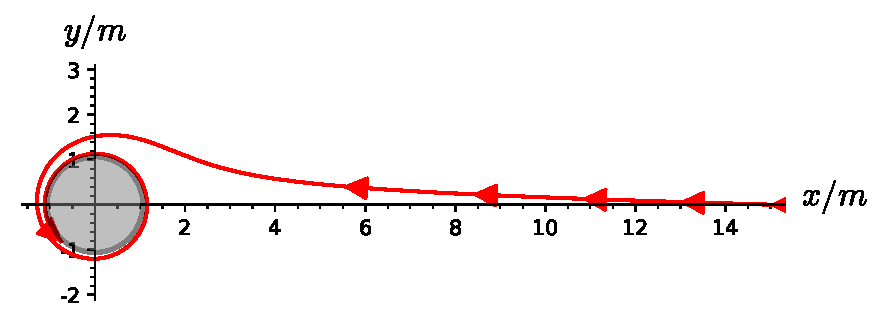
\includegraphics[width=0.7\textwidth]{gek_frame_dragging.pdf}}
\caption[]{\label{f:gek:frame_dragging} \footnotesize
Trajectory in the equatorial plane of an incoming timelike geodesic with
$E = \mu$, $L=0$ and $Q=0$, plunging into a Kerr black hole with $a = 0.998 \, m$.
The figure is drawn in terms
of the Cartesian Boyer-Lindquist coordinates $(x,y)$ defined by
Eq.~(\ref{e:gek:Cartesian_BL}) with $\th=\pi/2$ (equatorial plane)
and the grey disk marks the black hole region.
\textsl{[Figure generated by the notebook \ref{s:sam:Kerr_geod_plots}]}
}
\end{figure}

The Lense-Thirring effect is illustrated in Fig.~\ref{f:gek:frame_dragging}
which shows the trajectory a timelike particle with $L=0$
which is asymptotically at rest (marginally bound particle, having $E=\mu$,
to be discussed in Sec.~\ref{s:gek:r-motion}). The trajectory is initialy
radial, but as $r$ decreases, $\D\ph/\D t$ increases according to formula
(\ref{e:gek:dphdt_frame_dragging}).
In Fig.~\ref{f:gek:frame_dragging} and in all figures of this chapter, we are
using the \defin{Cartesian Boyer-Lindquist coordinates}\index{Cartesian!Boyer-Lindquist coordinates}
$(t,x,y,z)$, which are
defined in the $r>0$ region of Kerr spacetime and are related to the
Boyer-Lindquist coordinates $(t,r,\th,\ph)$ by the standard transformation
from spherical to Cartesian coordinates:
\be \label{e:gek:Cartesian_BL}
    x := r\sin\th\cos\ph,\qquad
    y := r\sin\th\sin\ph,\qquad
    z := r\cos\th .
\ee

We note that, at a given point $(r,\th)$, the angular velocity (\ref{e:gek:dphdt_frame_dragging})
coincides with that of the zero-angular momentum observer (ZAMO) at that point
[compare Eq.~(\ref{e:ker:omega_ZAMO})].

\subsection{Winding near the event horizon and the inner horizon}

Let us consider a null or timelike geodesic $\Li$ in the vicinity of the
black hole event horizon $\Hor$.
On $\Hor$, $r=r_+$ and $\Delta = 0$. Then, the term
$\Delta^{-1}$ in Eq.~(\ref{e:gek:dtdl}) makes $\D t/\D\lambda$ diverge as
$r\to r_+$, except in the very special where $(r_+^2 + a^2)E - aL = 0$, which
is equivalent to $E = \Omega_H L$ according to Eq.~(\ref{e:ker:def_OmegaH}).
Similarly, $\D\ph/\D\lambda$, as given by Eq.~(\ref{e:gek:dphdl}), diverges
as $r\to r_+$, except for $E = \Omega_H L$. These two divergences are not
a pathology of $\Li$ per se; they
reflect merely the singularity of Boyer-Lindquist coordinates $(t,r,\th,\ph)$ at $\Hor$
(cf.  Sec.~\ref{s:ker:singularities}). However, we read on Eqs.~(\ref{e:gek:dtdl}) and
(\ref{e:gek:dphdl}) that the ratio
$\left. \D\ph/\D t \right| _{\Li} := \D\ph/\D\lambda \times (\D t/\D\lambda)^{-1}$
converges to a finite value:
\be \label{e:gek:lim_dphdt_Hor}
    \lim_{r\to r_+} \left. \derd{\ph}{t} \right| _{\Li} = \frac{a}{r_+^2 + a^2} = \Omega_H ,
\ee
where the second equality follows from Eq.~(\ref{e:ker:def_OmegaH}), letting
the black hole rotation velocity $\Omega_H$ appear.
Hence we conclude that
\begin{greybox}
Any null or timelike geodesic that approaches the event horizon $\Hor$
is winding around it in terms of the Boyer-Lindquist coordinates at exactly the black hole rotation velocity $\Omega_H$.
\end{greybox}

\begin{remark}
For a timelike geodesic on a circular orbit, we have argued in Sec.~\ref{s:ges:circular_orbits}
that $\left. \D\ph/\D t \right| _{\Li}$ is the angular velocity of
as seen by an asymptotic inertial observer. The reasoning was
given in the Schwarzschild spacetime context but it actually involved only
the spacetime symmetry by translation in $t$, so it is applicable here.
\end{remark}

\begin{figure}
\centerline{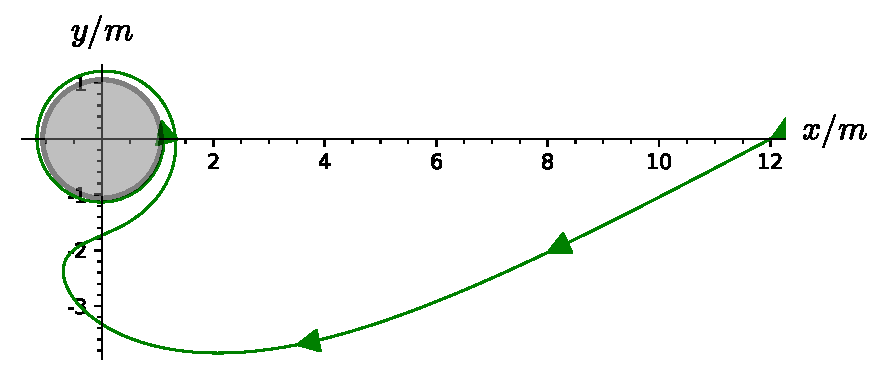
\includegraphics[width=0.7\textwidth]{gek_winding_null.pdf}}
\caption[]{\label{f:gek:winding_null} \footnotesize
Trajectory in the equatorial plane of an incoming null geodesic with
$L=-6E < 0$ and $Q=0$, plunging into a Kerr black hole with $a = 0.998 \, m$.
Note the turning point in $\ph$ and the final winding in the direction of the black
rotation (counterclockwise in the figure). The figure is drawn in terms
of the Cartesian Boyer-Lindquist coordinates $(x,y)$ defined by
Eq.~(\ref{e:gek:Cartesian_BL}) with $\th=\pi/2$ (equatorial plane)
and the grey disk marks the black hole region.
\textsl{[Figure generated by the notebook \ref{s:sam:Kerr_geod_plots}]}
}
\end{figure}


\begin{remark}
When $a\not=0$,
a geodesic that starts far from the black hole with
$\left. \D\ph/\D t \right| _{\Li} < 0$ [according to Eq.~(\ref{e:gek:dphdl}) with $r\gg m$,
this occurs for $L <0$]
must necessarily have a turning point in $\ph$
if it reaches the event horizon, in order to fulfill (\ref{e:gek:lim_dphdt_Hor}),
where $\Omega_H$ is positive. This is illustrated in Fig.~\ref{f:gek:winding_null}
and is in sharp contrast with the Schwarzschild case, where $\ph$ is always
a monotonous function of $\lambda$, as shown in Sec.~\ref{s:ges:eq_to_be_solved}.
\end{remark}


\begin{remark}
The winding property does not hold for the Kerr or 3+1 Kerr coordinates. Indeed,
we have seen in Sec.~\ref{s:ker:principal_geod} that the
ingoing principal null geodesics $\Li^{\rm in}_{(v,\th,\tph)}$ are geodesics
along which $\tph$ is constant. They are therefore not winding in terms
of neither the Kerr coordinates $(v,r,\th,\tph)$ nor the 3+1 Kerr ones $(\ti,r,\th,\tph)$.
This difference of (coordinate) behaviour is understandable if one considers
the diverging behaviour in $\Delta^{-1}$ of the
relation $\D \tph = \D \ph + a/\Delta\, \D r$ [Eq.~(\ref{e:ker:Kerr_coord_tph})]
between the angular coordinates $\ph$ and $\tph$.
\end{remark}

Regarding the Boyer-Lindquist coordinate behaviour in the vicinity of the inner
horizon $\Hor_{\rm in}$ (corresponding to the second root $r_-$ of $\Delta$), we deduce
from
Eqs.~(\ref{e:gek:dtdl}) and
(\ref{e:gek:dphdl}) that
\be
    \lim_{r\to r_-} \left. \derd{\ph}{t} \right| _{\Li} = \frac{a}{r_-^2 + a^2} = \Omega_{\rm in} ,
\ee
where the second equality follows from Eq.~(\ref{e:ker:def_Omega_in}); it involves
the rotation velocity $\Omega_{\rm in}$ of the inner horizon $\Hor_{\rm in}$.
Hence
\begin{greybox}
Any null or timelike geodesic that approaches the inner horizon $\Hor_{\rm in}$
is winding around it in terms of the Boyer-Lindquist coordinates at exactly the
rotation velocity $\Omega_{\rm in}$ of $\Hor_{\rm in}$.
\end{greybox}

\subsection{Asymptotic $r$-values and $\th$-values} \label{s:gek:asymptotic_values}

Let $\Li$ be a geodesic
and $p_0$ a point of $\Li$ at which $r$ varies,
i.e. such that $R(r_0) \neq 0$, where $r_0 = r(p_0)$.
Let us assume that $\Li$ comes close to $r=r_1$, where
$r_1$ is a double root of $R$, i.e. fulfils $R(r_1)=0$, $R'(r_1)=0$ and
$R''(r_1)\neq 0$, such that $R(r) > 0$ on the interval $[r_0, r_1)$.
Let us reconsider the argument in Sec.~\ref{s:gek:Mino_time}
that lead to extend the integral
(\ref{e:gek:lp_int_dr_ov_R}) to $r=r_1$, where $r_1$ corresponded to
a simple root of $R$ ($R(r_1)=0$ and $R'(r_1)\neq 0$).
For a double root,
the integral in the right-hand side of Eq.~(\ref{e:gek:lp_int_dr_ov_R}) with $r=r_1$ behaves
near $r_1$ as
\[
    \frac{\sqrt{2}}{\sqrt{R''(r_1)}} \int_{r_0}^{r_1} \frac{\D \bar{r}}{r_1 - \bar{r}} ,
\]
which is a divergent improper integral. If $r_1$ is a higher order root of $R$,
the divergence is even worse, being triggered by a higher power of $1/(r_1 - \bar{r})$.
Consequently, Eq.~(\ref{e:gek:lp_int_dr_ov_R}) with $r=r_1$
implies that the Mino parameter diverges: $\lambda'\to +\infty$. Since $\rho^2 > 0$,
provided that $\rho^2$
does not tend to $0$ (the ring singularity) as $\lambda'\to +\infty$, this
implies that the affine parameter $\lambda$ tends to $+\infty$ as well, given
the relation (\ref{e:gek:def_Mino_time}) between the two parameters.
Hence we conclude
\begin{greybox}
Let $\Li$ be a geodesic of Kerr spacetime that does not lie at a fixed value of $r$
and let $R(r)$ be the associated polynomial
(\ref{e:gek:def_R_Q}).
A point away from the ring singularity $\ring$ and of $r$-coordinate $r_1$
such that both $R(r_1) = 0$ and $R'(r_1) = 0$
can only be reached asymptotically by $\Li$, i.e. in the limit
$\lambda\to \pm\infty$ of the affine parameter
$\lambda$. We call $r_1$ an \defin{asymptotic $r$-value}\index{asymptotic!$r$-value} of the geodesic $\Li$.
\end{greybox}
This property explains why $R(r_0) = 0$ and $R'(r_0) \neq 0$ is a necessary condition
to have a $r$-turning point (cf. Remark~\ref{r:gek:der_r_analytic} on page~\pageref{r:gek:der_r_analytic}).

By the same reasoning, we have
\begin{greybox}
Let $\Li$ be a geodesic of Kerr spacetime that does not lie at a fixed value of $\th$ and let
$\Theta(\th)$ be the associated function
(\ref{e:gek:def_Theta}).
A point away from the ring singularity $\ring$ and of $\th$-coordinate $\th_1$
such that both $\Theta(\th_1) = 0$ and $\Theta'(\th_1) = 0$
can only be reached asymptotically by $\Li$, i.e. in the limit
$\lambda\to \pm\infty$ of the affine parameter
$\lambda$. We call $\th_1$ an
\defin{asymptotic $\th$-value}\index{asymptotic!$\th$-value} of the geodesic $\Li$.
\end{greybox}



\subsection{$\th$-motion} \label{s:gek:th_motion}

We start by analysing the variation of the $\th$ coordinate along a geodesic,
as governed by the decoupled equation
(\ref{e:gek:dthdl_Mino}), since this provides some constraints
to discuss later the $r$-motion.

Given expression~(\ref{e:gek:Theta_Q}) for $\Theta(\th)$,
the first-order equation of motion (\ref{e:gek:dthdl_Mino}) can be rewritten as
\be \label{e:gek:th_eff_potential}
    \encadre{ \left( \derd{\th}{\lambda'} \right)^2 + V(\th) = Q },
\ee
with
\be \label{e:gek:def_V_th}
  \encadre{  V(\th) := \cos^2\th \left[ a^2(\mu^2 - E^2) + \frac{L^2}{\sin^2\th} \right] }.
\ee
Note that $V(\th)$ is related to $\Theta(\th)$ by
\be
    \Theta(\th) = Q - V(\th).
\ee
In particular, the $\th$-turning points (cf. Sec.~\ref{s:gek:turning_points})
are characterized by
$V(\th) = Q$ and $V'(\th) \neq 0$, while the asymptotic $\th$-values
(cf. Sec.~\ref{s:gek:asymptotic_values})
correspond to $V(\th) = Q$ and $V'(\th) = 0$.

We recognize in Eq.~(\ref{e:gek:th_eff_potential}) the first integral of a
(non-relativistic) 1-dimensional motion in the potential $V(\th)$, which we
shall call the
\defin{effective $\th$-potential}\index{effective!$\th$-potential}.
The discussion of the geodesic $\th$-motion
is then based on the properties of that potential, $Q$
in the right-hand side of Eq.~(\ref{e:gek:th_eff_potential})
playing the role of
the constant ``total energy''. Since $(\D\th / \D\lambda')^2 \geq 0$,
Eq.~(\ref{e:gek:th_eff_potential})  implies
\be \label{e:gek:V_leq_Q}
    V(\th) \leq Q .
\ee
Accordingly, given a plot of $V(\th)$, as in Figs.~\ref{f:gek:th_pot_L_0} and
\ref{f:gek:th_pot_L_non0}, the allowed range of $\th$ is determined
by the part of the graph of $V(\th)$ that lies below
the horizontal line of ordinate equal to $Q$.

We shall distinguish the
case $L=0$ from the case $L\not=0$, since they lead
to different shapes of the potential $V(\th)$.



\subsubsection{Geodesics with $L=0$}

If $L=0$, the effective $\th$-potential reduces to $V(\th)=a^2(\mu^2 - E^2)\cos^2\th$.
We have then three subcases:

\begin{itemize}
\item \textbf{Case} $a^2 (E^2 - \mu^2) < 0 \iff a\neq 0 \ \mbox{and}\ |E| < \mu$:
the corresponding graph of $V(\th)$ is shown in
Fig.~\ref{f:gek:th_pot_L_0} (left part); we deduce immediately from it that
$Q\geq 0$, with
\begin{itemize}
\item $Q=0$: the motion is confined to the equatorial
plane $\th=\pi/2$; since it corresponds to a minimum of the effective potential, this
is a stable configuration.
\item $0<Q< a^2(\mu^2 - E^2)$: $\th$ oscillates between
two $\th$-turning points, which are symmetric about the equatorial plane\footnote{The index ${\rm m}$
in $\th_{\rm m}$ stands for \emph{minimal}.}:
$\th_{\rm m} := \arccos\sqrt{Q/(a^2(\mu^2 - E^2))}$
and $\pi-\th_{\rm m}$ (cf. the trajectory $Q=Q_1$ in Fig.~\ref{f:gek:th_pot_L_0}, left).
\item $Q = a^2(\mu^2 - E^2)$: $\th=0$ and $\th=\pi$
are either unstable positions or
asymptotic $\th$-values (cf. Sec.~\ref{s:gek:asymptotic_values}), i.e.
the geodesic reaches the rotation axis for $\lambda\to\pm\infty$.
\item $Q > a^2(\mu^2 - E^2)$:
the range of $\th$ is not limited (cf. the trajectory $Q=Q_2$ in Fig.~\ref{f:gek:th_pot_L_0}, left)
and each time the geodesic reaches the
rotation axis ($\th=0$ or $\th=\pi$),
it crosses it, since the velocity $\D\th / \D\lambda'$
does not vanish there. This leads to $\th < 0$ or $\th > \pi$; to keep $\th$
within the interval $[0,\pi]$, one shall use the identification
of the points $(\th, \ph)$, $(-\th, \ph+\pi)$ and $(\th-\pi, \ph+\pi)$,
which holds on the sphere $\mathbb{S}^2$.
\end{itemize}
\item \textbf{Case} $a^2 (E^2 - \mu^2) = 0 \iff a=0\ \mbox{or}\ |E|=\mu$:
$V(\th)=0$ and Eq.(\ref{e:gek:th_eff_potential})
reduces to $(\D\th/\D\lambda')^2 = Q$. This implies $Q\geq 0$
and the solution is $\th(\lambda') = \pm \sqrt{Q}\, \lambda' + \th_0$,
so that
\begin{itemize}
\item for $Q=0$, the geodesic lies at a constant value of $\th$, within the range
$[0,\pi]$;
\item for $Q>0$, $\th$ varies monotonically along the geodesic, which
therefore crosses the rotation
axis an infinite number of times.
\end{itemize}
\item \textbf{Case} $a^2 (E^2 - \mu^2) > 0 \iff a\neq 0 \ \mbox{and}\  |E|>\mu$:
the corresponding graph of $V(\th)$ is shown in
Fig.~\ref{f:gek:th_pot_L_0} (right part); the Carter constant must obey
$Q \geq - a^2 (E^2 - \mu^2)$, with
\begin{itemize}
\item $Q=-a^2(E^2 - \mu^2)$: only $\th=0$ and
$\th=\pi$ are possible and they correspond to minima of $V(\th)$;
the geodesic is then stably located on the rotation axis.
\item $-a^2(E^2 - \mu^2) < Q < 0$: the geodesic oscillates about the rotation
axis, without reaching the equator; one has either $\th\in[0,\th_{\rm v}]$ or
$\th\in [\pi - \th_{\rm v},\pi]$, with the turning point value\footnote{The index ${\rm v}$
in $\th_{\rm v}$ stands for \emph{vortical}, the definition of which is given at the end of this
section.}
$\th_{\rm v} := \arccos\sqrt{|Q|/(a^2(E^2 - \mu^2))} < \pi/2$ (cf. the trajectories $Q=Q_1$ in Fig.~\ref{f:gek:th_pot_L_0}, right).
\item $Q=0$: $\th=\pi/2$ is either an unstable position or
an asymptotic $\th$-value, i.e. the geodesic approaches the equatorial
plane when $\lambda\to\pm\infty$.
\item $Q>0$: $\th$ varies in all the range $[0,\pi]$; when
the geodesic reaches the rotation axis, it crosses it (cf. the trajectory $Q=Q_2$ in Fig.~\ref{f:gek:th_pot_L_0}, right).
\end{itemize}
\end{itemize}

\begin{figure}
\centerline{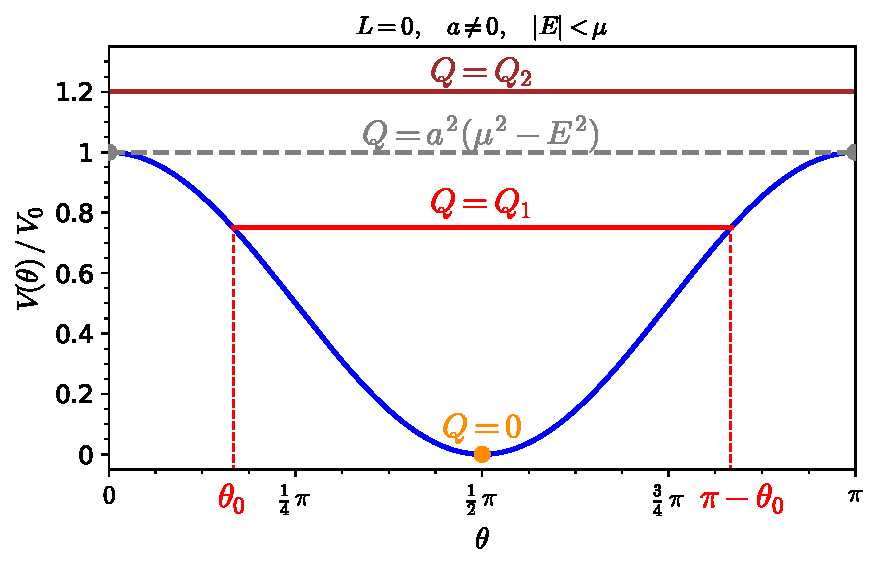
\includegraphics[height=0.24\textheight]{gek_th_pot_L_0_low_E.pdf}
\ 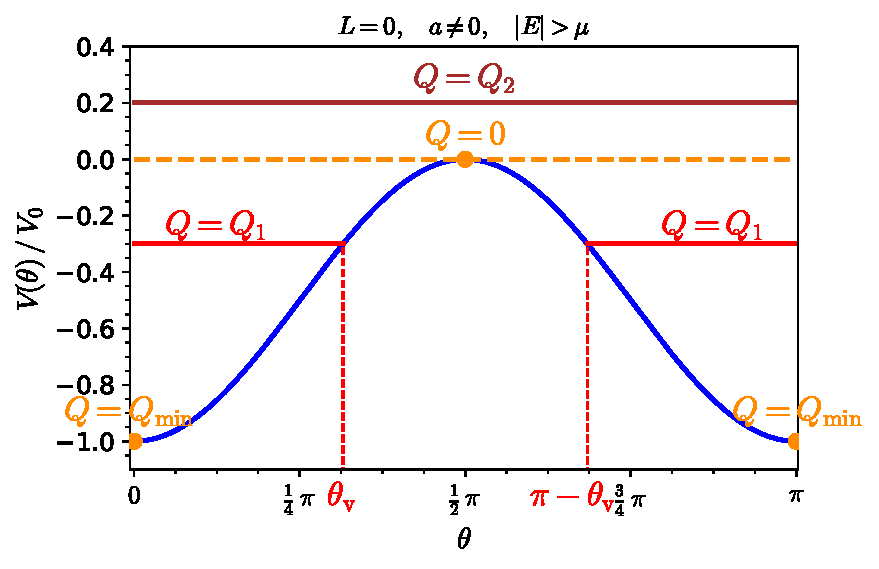
\includegraphics[height=0.24\textheight]{gek_th_pot_L_0_high_E.pdf}}
\caption[]{\label{f:gek:th_pot_L_0} \footnotesize
Effective $\th$-potential $V(\th)$ in the case $L=0$ and $a\neq 0$. $V(\th)$ is plotted
in units of $V_0 := a^2|\mu^2 - E^2|$.
The left figure is for $|E| < \mu$, with colored dots or horizontal lines
corresponding to geodesic trajectories for four values of the Carter constant $Q$:
$0$, $Q_1 = 0.75 V_0$, $a^2(\mu^2 - E^2)$ and $Q_2 = 1.2 V_0$.
The right figure is for $|E| > \mu$, with trajectories corresponding
to four values of $Q$: $Q_{\rm min} = -a^2(E^2 - \mu^2)$,
$Q_1 = -0.3 V_0$, $0$ and $Q_2 = 0.2 V_0$.
Dashed lines indicate trajectories with asympotic $\th$-values.
%\textsl{[Figure generated by the notebook \ref{s:sam:ges_eff_pot_null}]}
}
\end{figure}


\begin{figure}
\centerline{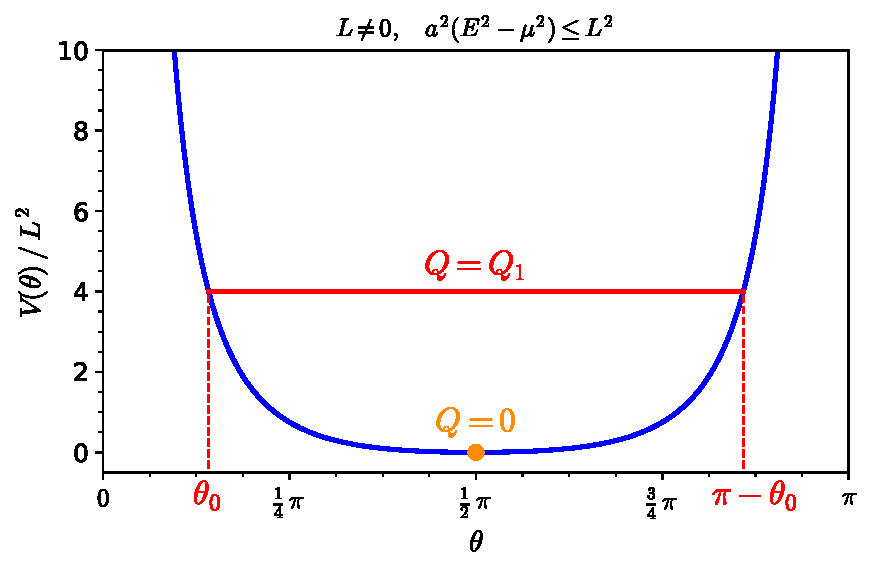
\includegraphics[width=0.49\textwidth]{gek_th_pot_high_L.pdf}
\ 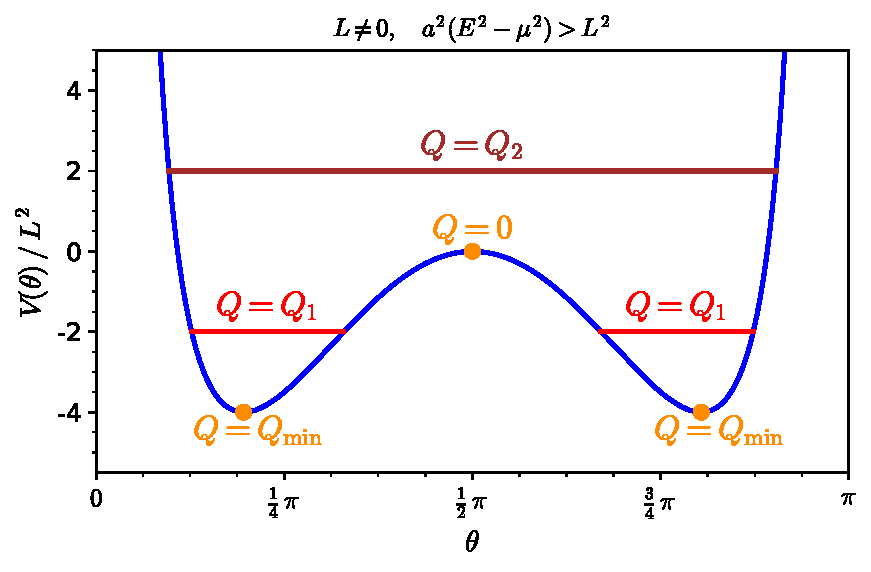
\includegraphics[width=0.49\textwidth]{gek_th_pot_low_L.pdf}}
\caption[]{\label{f:gek:th_pot_L_non0} \footnotesize
Effective $\th$-potential $V(\th)$ in the case $L\neq0$.
The left figure is for $L^2 \geq a^2(E^2 - \mu^2)$, with
with colored dots or horizontal lines
corresponding to geodesic trajectories for
two values of the Carter constant $Q$: $0$ and $Q_1= 4 L^2$.
The right figure is for $L^2 < a^2(E^2 - \mu^2)$, with trajectories corresponding
to four values of $Q$: $Q_{\rm min}$, $Q_1 = - 2 L^2$, $0$ and $Q_2 = 2 L^2$.
The dashed line ($Q=0$)
indicates the trajectory with an asympotic $\th$-value, which is $\pi/2$.
%\textsl{[Figure generated by the notebook \ref{s:sam:ges_eff_pot_null}]}
}
\end{figure}


\subsubsection{Geodesics with $L\not=0$}

When $L\not=0$, we see from expression~(\ref{e:gek:def_V_th}) that
$V(\th) \to +\infty$ when $\th\to 0$ or $\pi$.
We conclude immediately that the geodesic cannot reach the rotation axis
for $L\not=0$.
Moreover, we have
\[
    \derd{V}{\th} = - 2 \cos\th\sin\th \left[ a^2 (\mu^2 - E^2) + \frac{L^2}{\sin^4\th} \right] .
\]
The extrema of $V$ in $(0,\pi)$ are then given by
\be
    \derd{V}{\th} = 0 \iff
        \th = \frac{\pi}{2} \quad\mbox{or}\quad
        \sin^4\th = \frac{L^2}{a^2(E^2 - \mu^2)} .
\ee
We are thus led to distinguish two cases, depending whether or not the
equation involving $\sin^4\th$ has solutions distinct from $\pi/2$:
\begin{itemize}
\item \textbf{Case} $L^2 \geq a^2(E^2 - \mu^2) \iff a=0\
\mbox{or}\ |E| \leq \sqrt{\mu^2 + \frac{L^2}{a^2}}$: the only extremum solution is
$\th=\pi/2$.
Its value is $V(\pi/2)=0$ and it is
necessarily a minimum, since $V(\th) \to +\infty$ at the boundaries of the
interval $[0,\pi]$ (cf. left part of Fig.~\ref{f:gek:th_pot_L_non0}).
Hence one must have $Q\geq 0$, with
\begin{itemize}
\item $Q=0$: the geodesic stays stably in the
equatorial plane.
\item $Q>0$: the geodesic oscillates about the equatorial plane,
between two turning points at $\th=\th_{\rm m}$ and $\pi-\th_{\rm m}$, $\th_{\rm m}$ being the solution
of $V(\th_{\rm m}) = Q$ in $(0,\pi/2)$ (cf. the trajectory $Q=Q_1$ in Fig.~\ref{f:gek:th_pot_L_non0}, left).
\end{itemize}
\item \textbf{Case} $L^2 < a^2(E^2 - \mu^2)  \iff a\neq 0\
\mbox{and}\ |E| > \sqrt{\mu^2 + \frac{L^2}{a^2}}$: $V(\th)$ has three extrema (cf. right part of Fig.~\ref{f:gek:th_pot_L_non0}), which are located at
$\th=\th_*$, $\pi/2$ and $\pi-\th_*$ with
\be \label{e:gek:theta_star}
    \th_* := \arcsin\sqrt{\frac{|L|}{a\sqrt{E^2 - \mu^2}}}
    \quad\mbox{and}\quad 0 < \th_* < \frac{\pi}{2} .
\ee
$\th_*$ and $\pi-\th_*$ correspond to the minimum of $V(\th)$,
while $\pi/2$ corresponds to a local maximum. The minimum is
$V(\th_*) = (1-\sin^2\th_*)(a^2(\mu^2-E^2) + L^2/\sin^2\th_*) = - (a \sqrt{E^2 - \mu^2} - |L|)^2$.
This is necessary the minimal value of $Q$ [cf. Eq.~(\ref{e:gek:V_leq_Q})]:
\be  \label{e:gek:Q_min_prov}
    Q_{\rm min} = - \left( a \sqrt{E^2 - \mu^2} - |L| \right) ^2 .
\ee
We have then (cf. right panel of Fig.~\ref{f:gek:th_pot_L_non0})
\begin{itemize}
\item $Q = Q_{\rm min}$: the geodesic stays stably at a fixed value of $\th$,
either $\th_*$ or $\pi - \th_*$.
\item $Q_{\rm min} < Q < 0$: the geodesic oscillates between two $\th$-turning
points either in the Northern
hemisphere ($\th < \pi/2$) or the Southern one ($\th > \pi/2$), without reaching
the equator nor the rotation axis (cf. the trajectories $Q=Q_1$ in Fig.~\ref{f:gek:th_pot_L_non0}, right).
\item $Q=0$: the geodesic lies unstably in the equatorial plane or
moves asymptotically towards it (possibly after a turning point at $\th_{\rm m}\neq\pi/2$), $\pi/2$ being an asymptotic $\th$-value, since $\Theta'(\pi/2) = - V'(\pi/2)=0$
(cf. Sec.~\ref{s:gek:asymptotic_values}).
\item $Q>0$: the geodesic oscillates about the equatorial plane,
between two turning points at $\th=\th_{\rm m}$ and $\pi-\th_{\rm m}$, $\th_{\rm m}$ being the solution
of $V(\th_{\rm m}) = Q$ in $(0,\pi/2)$ (cf. the trajectory $Q=Q_2$ in Fig.~\ref{f:gek:th_pot_L_non0}, right).
\end{itemize}
\end{itemize}

\subsubsection{Expression of the $\th$-turning points}

The $\th$-turning points $\th_{\rm m}$ and $\th_{\rm v}$ mentioned above are solutions of
$\Theta(\th) = 0$ and  $\Theta'(\th) \neq 0 $ [Eq.~(\ref{e:gek:def_th_turning})]. We search only for
$\th$-turning points with $0 < \th < \pi/2$, since $0$ and $\pi/2$ cannot be
$\th$-turning points (for $\Theta'(0) = 0 $ and $\Theta'(\pi/2) = 0$) and
$\th$-turnings points with  $\pi/2 < \th < \pi$ are deduced from those
with $0 < \th < \pi/2$ by $\th \mapsto \pi - \th$
(symmetry with respect to the equatorial plane).
Using expression~(\ref{e:gek:Theta_Q})
for $\Theta$ and introducing
\be
    x := \cos^2\th ,
\ee
the equation $\Theta(\th) = 0$ is equivalent to
\be \label{e:gek:quadrat_x}
    a^2 (E^2 - \mu^2) x^2 + \left[ L^2 + Q - a^2 (E^2 - \mu^2) \right] x - Q = 0 .
\ee
If $a^2 (E^2 - \mu^2) = 0$, the solution is $x = Q/(L^2 + Q)$. Moreover, in this
case one has necessarily $Q \geq 0$, so that $0 \leq x \leq 1$ and
the unique solution in $(0,\pi/2)$ is
\be \label{e:gek:th0_a2E2mu2_zero}
     \encadre{\th_{\rm m} = \arccos\sqrt{\frac{Q}{L^2 + Q}} . }_{\, a^2 (E^2 - \mu^2) = 0}
\ee
In the rest of this section, we assume that $a^2 (E^2 - \mu^2) \neq 0$.
Equation~(\ref{e:gek:quadrat_x}) is then a quadratic equation in $x$, the discriminant
of which is
\begin{align}
\mathit{\Delta} & = \left[ L^2 + Q - a^2 (E^2 - \mu^2) \right]^2 + 4 Q a^2 (E^2 - \mu^2) \nonumber \\
  & = \left[ L^2 + Q + a^2 (E^2 - \mu^2) \right]^2 - 4 L^2 a^2 (E^2 - \mu^2) . \nonumber
\end{align}
It turns out that $\mathit{\Delta}$ is always non-negative. Indeed, from the second equality
above, we have clearly $\Delta \geq 0$ if $a^2(E^2 - \mu^2) \leq 0$. In the complementary
case, i.e. when $a^2(E^2 - \mu^2) > 0$, then $\mathit{\Delta} \geq 0$ as soon
as $Q \geq Q_2$, where $Q_2$ is the larger of the two roots of $\mathit{\Delta}$
considered as a quadratic polynomial in $Q$. Again, considering the second equality
in the expression of $\mathit{\Delta}$, we have
$Q_2 = - L^2 - a^2 (E^2 - \mu^2) + 2 |L| a \sqrt{E^2 - \mu^2} = - (|L| - a \sqrt{E^2 - \mu^2} )^2$.
In view of Eq.~(\ref{e:gek:Q_min_prov}), we realize that $Q_2 = Q_{\rm min}$,
so that $Q\geq Q_2$ always holds and $\Delta\geq 0$.
Accordingly the two roots of Eq.~(\ref{e:gek:quadrat_x}) are real and are
given by
\be \label{e:gek:th_turn_x_pm}
    x_{\pm} = \frac{1}{2} \left( 1 - \frac{L^2 + Q}{a^2 (E^2 - \mu^2)}
        \pm \sqrt{ \left[1 - \frac{L^2 + Q}{a^2 (E^2 - \mu^2)}\right] ^2
        + \frac{4Q}{a^2 (E^2 - \mu^2)}} \right) .
\ee
Since $x := \cos^2\th$ and $\th=0$ and $\th=\pi/2$ cannot correspond
to a $\th$-turning point,
acceptable solutions must obey
\be \label{e:gek:th_turn_x_pm_range}
    0 < x_{\pm} < 1 .
\ee

For $L=0$, Eq.~(\ref{e:gek:th_turn_x_pm}) simplifies to\footnote{A switch between
$x_+$ and $x_-$ is performed if $1 + Q/(a^2(E^2 - \mu^2)) < 0$.}
\[
    x_+ = 1 \qand x_- = - \frac{Q}{a^2(E^2 - \mu^2)}
\]
Now, $x_+ = 1$ is excluded by (\ref{e:gek:th_turn_x_pm_range}). There remains
only $x_-$, leading to the turning point value found in the
$L=0$ cases discussed above, which we can combine into a single formula:
\be \label{e:gek:th0_L_zero}
   \encadre{ \th_{\rm m} = \th_{\rm v} = \arccos \sqrt{\frac{Q}{a^2 (\mu^2 - E^2)}} . }_{\, L=0}
\ee
This formula assumes that $0 < Q/(a^2 (\mu^2 - E^2)) < 1$ (as for the trajectories
$Q=Q_1$ in both panels of Fig.~\ref{f:gek:th_pot_L_0}),
otherwise there
is no $\th$-turning point (as for the trajectories $Q=Q_2$ in both panels of
Fig.~\ref{f:gek:th_pot_L_0}).
More precisely, for $Q > 0$ and $\mu^2 - E^2 > 0$, it leads to $\th_{\rm m}$, while
for $Q<0$ and $\mu^2 - E^2 < 0$, it leads to $\th_{\rm v}$.

For $L\neq 0$, one shall distinguish between two cases, since the case $|E| = \mu$
has been covered above [Eq.~(\ref{e:gek:th0_a2E2mu2_zero})]:
\begin{itemize}
\item if $|E| < \mu$, then only $x_-$ fulfils the criterion (\ref{e:gek:th_turn_x_pm_range}),
leading to the turning point value:
\be \label{e:gek:th0_E_lt_mu}
    \encadre{ \th_{\rm m} = \arccos \sqrt{ \frac{1}{2} \left[ 1 + \frac{L^2 + Q}{a^2 (\mu^2 - E^2)}
        - \sqrt{ \left[1 + \frac{L^2 + Q}{a^2 (\mu^2 - E^2)}\right] ^2
        - \frac{4Q}{a^2 (\mu^2 - E^2)}} \right] }}
\ee
\item if $|E| > \mu$, then $x_+$ always fulfils the criterion (\ref{e:gek:th_turn_x_pm_range}),
leading to the turning point value:
\be \label{e:gek:th0_E_gt_mu}
    \encadre{\th_{\rm m} =  \arccos  \sqrt{   \frac{1}{2} \left[ 1 - \frac{L^2 + Q}{a^2 (E^2 - \mu^2)}
        + \sqrt{ \left[1 - \frac{L^2 + Q}{a^2 (E^2 - \mu^2)}\right] ^2
        + \frac{4Q}{a^2 (E^2 - \mu^2)}} \right]  } } .
\ee
If, in addition $Q<0$, then $x_-$ also fulfils (\ref{e:gek:th_turn_x_pm_range})
and we get a second turning point value (cf. the case $Q=Q_1$ in the
right panel of Fig.~\ref{f:gek:th_pot_L_non0}):
\be \label{e:gek:th1}
    \encadre{\th_{\rm v} =  \arccos  \sqrt{  \frac{1}{2} \left[ 1 - \frac{L^2 + Q}{a^2 (E^2 - \mu^2)}
        - \sqrt{ \left[1 - \frac{L^2 + Q}{a^2 (E^2 - \mu^2)}\right] ^2
        + \frac{4Q}{a^2 (E^2 - \mu^2)}} \right]  } } .
\ee
\end{itemize}
\begin{remark}
At the limit $L\to 0$, formulas (\ref{e:gek:th0_E_lt_mu}) and
(\ref{e:gek:th1}) reduce both to (\ref{e:gek:th0_L_zero}).
\end{remark}


\subsubsection{Summary}

We can summarize the above results by
\begin{greybox}
\begin{itemize}
\item A geodesic $\Li$ of Kerr spacetime cannot encounter the rotation axis unless it has $L=0$.
\item If $L^2 \geq a^2 (E^2 - \mu^2)$,
the Carter constant $Q$ is necessarily non-negative:
\be \label{e:gek:Q_nonnegative}
    Q \geq 0 .
\ee
\item The Carter constant $Q$ can take negative values only if
$L^2 < a^2 (E^2 - \mu^2)$, which implies $a\neq 0$
and $|E| > \mu$; the range of $Q$ is then
limited from below:
\be
    Q \geq Q_{\rm min} = - \left( a \sqrt{E^2 - \mu^2} - |L| \right) ^2.
\ee
A geodesic with $Q<0$ is called \defin{vortical}\index{vortical geodesic}; it
never encounters the equatorial plane.
\item If $Q>0$, $\Li$ oscillates symmetrically about the equatorial plane,
between two $\th$-turning points, at $\th=\th_{\rm m}$ and $\th=\pi-\th_{\rm m}$, where $\th_{\rm m}\in(0,\pi/2)$
is given by Eq.~(\ref{e:gek:th0_a2E2mu2_zero})
for $a^2(E^2 - \mu^2) = 0$, Eq.~(\ref{e:gek:th0_L_zero}) for $L=0$ and
$Q < a^2(\mu^2 - E^2)$, Eq.~(\ref{e:gek:th0_E_lt_mu}) for $|E|<\mu$
and Eq.~(\ref{e:gek:th0_E_gt_mu}) for $|E|>\mu$,
except for two subcases with $L=0$: (i) $Q = a^2 (\mu^2 - E^2)$: $\Li$
lies unstably along the rotation axis or approaches it asymptotically
and (ii) $Q >a^2(\mu^2 - E^2)$: $\Li$
crosses repeatedly the rotation axis, with $\th$ taking all values in the
range $[0,\pi]$.
\item If $Q=0$, $\Li$ is stably confined to the equatorial plane
for $L^2 > a^2 (E^2 - \mu^2)$ or $L^2 = a^2 (E^2 - \mu^2) \neq 0$;
for $L^2 < a^2 (E^2 - \mu^2)$, $\Li$ either lies unstably in the equatorial
plane or approaches it asymptotically from one side, while for
$L^2 = a^2 (E^2 - \mu^2) = 0$,
$\Li$ lies at a constant value $\th=\th_0\in[0,\pi]$.
\item If $Q_{\rm min} < Q < 0$, $\Li$ never encounters the equatorial plane,
having a $\th$-motion entirely confined either to the Northern hemisphere
($0<\th<\pi/2$) or to
the Southern one ($\pi/2<\th<\pi$); if $L\neq 0$, $\Li$ oscillates between
two $\th$-turning points, at $\th=\th_{\rm m}$ and $\th=\th_{\rm v}$ (Northern hemisphere)
or at $\th=\pi-\th_{\rm v}$ and $\th=\pi-\th_{\rm m}$ (Southern hemisphere), where
$\th_{\rm m}$ and $\th_{\rm v}$ are given by Eqs.~(\ref{e:gek:th0_E_gt_mu}) and
(\ref{e:gek:th1}) respectively; if $L=0$,
$\Li$ oscillates about the rotation axis, with a $\th$-turning point at
$\th=\th_{\rm v}$ or $\th = \pi - \th_{\rm v}$, where $\th_{\rm v}$
is given by Eq.~(\ref{e:gek:th0_L_zero}).
\item If $Q = Q_{\rm min}$, $\Li$ lies stably at a constant value $\th=\th_*$
or $\th = \pi - \th_*$, with $\th_*\in [0, \pi/2)$%]$
\ given by\footnote{This is Eq.~(\ref{e:gek:theta_star})
generalized to encompass the case $L=0$.}
\be
     \th_* := \arcsin\sqrt{\frac{|L|}{a\sqrt{E^2 - \mu^2}}} .
\ee
\end{itemize}
\end{greybox}

\begin{remark}
We could have deduced that $L=0$ is a necessary condition for a geodesic
to encounter the rotation axis without studying the potential $V(\th)$. Indeed,
by definition, $L = \w{\eta}\cdot\w{p}$ [Eq.~(\ref{e:gek:def_L})], with the Killing
vector $\w{\eta}$ being zero on the rotation axis, since the latter is
pointwise invariant under the action of the rotation group $\mathrm{SO}(2)$.
Hence $L=0$ on the rotation axis. Since $L$ is constant along the geodesic,
the result follows immediately.
\end{remark}

\begin{remark}
That a vortical geodesic never intersects the equatorial plane has been
obtained by examining the various cases $Q<0$. This result can be derived
directly from the constraint $\Theta(\th)\geq 0$ [Eq.~(\ref{e:gek:Theta_non_neg})],
by noticing the identity
$\Theta(\pi/2) = Q$, which follows immediately from Eq.~(\ref{e:gek:Theta_Q}).
\end{remark}

\begin{example}[Schwarzschild geodesics]
It is instructive to apply the above results to $a=0$ and recover
the geodesics in Schwarzschild spacetime studied in Chaps.~\ref{s:ges} and \ref{s:gis}.
There, spherical symmetry was used to select the coordinates $(t,r,\th,\ph)$ so that
the geodesic was confined to the hyperplane $\th=\pi/2$. Consequently there was
no $\th$-motion. Here, we keep the coordinates $(t,r,\th,\ph)$ fixed and do not
assume that they are adapted to the geodesic $\Li$ under consideration. So $\th$
may vary along $\Li$. In Schwarzschild spacetime, the Carter constant $Q$
is always non-negative, since the inequality $L^2 \geq a^2(E^2-\mu^2)$ is
trivially satisfied for $a=0$ [cf. Eq.~(\ref{e:gek:Q_nonnegative})].\\
If $Q=0$, then for $L=0$, $\Li$ lies at a constant value of $\th$: this actually
corresponds to a purely radial geodesic. Indeed,
the total angular momentum measured in the asymptotic region is $\w{L}_{\rm tot} = 0$
in that case [set $Q=0$, $L=0$ and $a=0$ in Eq.~(\ref{e:gek:Q_Ltot2_L2})].
If $L\neq 0$, still with $Q=0$,
$\Li$ lies stably in the equatorial plane (this is the only possibility for $a=0$ among
the $Q=0$ cases listed above).\\
If $Q>0$, then $L=0$ is necessarily the subcase (ii) listed above:
$\Li$ crosses repeatedly the $z$-axis ($\th\in\{0,\pi\}$); this corresponds to the case where
the orbital plane contains the $z$-axis. All the angular momentum measured asymptotically
is then contained in $Q$ [cf. Eq.~(\ref{e:gek:Q_Ltot2_L2})].
For $Q>0$ and $L\neq 0$, $\Li$ oscillates symmetrically about the equatorial
plane: this is the case where the orbital plane is inclined by an angle
$\iota\in(0,\pi/2)$
with respect to the equatorial plane; the $\th$-turning point of $\Li$ is then
$\th_{\rm m} = \pi/2-\iota$.
\end{example}


\subsection{$r$-motion} \label{s:gek:r-motion}

The $r$-part of geodesic motion is constrained by Eq.~(\ref{e:gek:R_non_neg}):
$R(r) \geq 0$. Let us expand expression (\ref{e:gek:def_R_Q})
for the quartic polynomial $R(r)$ in powers of $r$:
\be \label{e:gek:R_r_powers}
    \encadre{ R(r) = (E^2 - \mu^2) r^4 + 2 m \mu^2 r^3
     + \left[ a^2(E^2 - \mu^2) - Q - L^2 \right] r^2
     + 2m\left[ Q + (L - a E)^2 \right] r - a^2 Q} .
\ee

\subsubsection{Geodesics with $|E|<\mu$} \label{s:gek:bound_geod}

For $r\to \pm\infty$ and $|E|\neq \mu$,
we have $R(r) \sim (E^2 - \mu^2) r^4$ and in
particular $\lim_{r\to\pm\infty} R(r) = + \infty$ for $|E|>\mu$
and $\lim_{r\to\pm\infty} R(r) = - \infty$ for $|E|<\mu$. In the latter case,
the constraint $R(r) \geq 0$ cannot be satisfied for large values
of $|r|$. A geodesic with $|E|<\mu$ is therefore located within a bounded
region in terms of the radial coordinate $r$. Moreover, $|E|<\mu$
implies necessarily $L^2 > a^2 (E^2 - \mu^2)$, so that
the results of
Sec.~\ref{s:gek:th_motion} lead to $Q\geq 0$
[cf. Eq.~(\ref{e:gek:Q_nonnegative})]. Therefore, $-a^2 Q \leq 0$.
It follows then that $r$ cannot be negative.
Indeed, we see
on expression~(\ref{e:gek:R_r_powers}) that for $|E|<\mu$ (which implies $\mu>0$ and $Q\geq 0$) and $r<0$,
\[
    R(r) = \underbrace{(E^2 - \mu^2) r^4}_{<0} + \underbrace{2 m \mu^2 r^3}_{<0}
     + \underbrace{\left[ a^2 (E^2 - \mu^2) - Q - L^2 \right] r^2}_{\leq 0}
     + \underbrace{2m\left[ Q + (L - a E)^2 \right] r}_{\leq 0}
     \underbrace{-a^2 Q}_{\leq 0} ,
\]
which contradicts $R(r)\geq 0$.
Hence we conclude:
\begin{greybox}
Any geodesic $\Li$ with $|E|<\mu$ is necessarily timelike ($\mu >0$),
has a non-negative Carter constant $Q$,
is confined to the region $r\geq 0$ of Kerr spacetime
and cannot reach arbitrary large values of $r$. $\Li$ is called a
\defin{geodesic with a bound orbit}\index{geodesic!with a bound orbit}\index{bound!orbit},
or in short, a \defin{bound geodesic}\index{bound!geodesic}.
\end{greybox}
\begin{remark} \label{r:gek:bound_geod}
That $\Li$
cannot reach the asymptotic region $r\to +\infty$ could have been
found directly from the definition of $E$ as the ``energy at infinity''
of the particle $\mathscr{P}$ having $\Li$ as worldline
[Eq.~(\ref{e:gek:def_E})]. Indeed, since $\Li$ is timelike, the 4-momentum
of $\mathscr{P}$ is $\w{p} = \mu \w{u}$ [Eq.~(\ref{e:fra:p_m_u})], where
$\w{u}$ is the 4-velocity of $\mathscr{P}$, so that Eq.~(\ref{e:gek:def_E})
yields $E = - \mu\, \w{\xi}\cdot\w{u}$. Now, when $r\to +\infty$, $\w{\xi}$
tends to the 4-velocity of an inertial observer (cf. Sec.~\ref{s:ker:asymp_inertial_obs}).
If $\Li$ could reach the asymptotic region,
the scalar
product of the two 4-velocities $\w{\xi}$ and
$\w{u}$ would be necessarily lower or equal to $-1$, or equivalently
$\Gamma := - \w{\xi}\cdot\w{u} \geq 1$ (the proof lies in expression
(\ref{e:fra:Gam_V2}) of $\Gamma$ with $0\leq \w{V}\cdot\w{V} < 1$), so that
we would have $E \geq \mu$, which contradicts $|E|<\mu$.
\end{remark}

\subsubsection{Geodesics with $|E|=\mu$}

Contrary to the case $|E|<\mu$, a geodesic with $|E|=\mu$ can be null,
provided it has $E=0$
(cf. Example~\ref{x:gek:null_generator_hor} on page~\pageref{x:gek:null_generator_hor}).
We have
\begin{greybox}
Any geodesic with $|E|=\mu$ has $Q\geq 0$ and is necessarily confined
to the region $r\geq 0$ of Kerr spacetime.
\end{greybox}
\begin{proof}
$Q\geq 0$ follows directly from the criteria $|E| \leq \sqrt{\mu^2 + {L^2}/{a^2}}$
[cf. Eq.~(\ref{e:gek:Q_nonnegative})],
which is evidently fulfilled for $|E|=\mu$.
Furthermore, for $|E|=\mu$, expression (\ref{e:gek:R_r_powers}) for $R(r)$
simplifies to
\[
    R(r) =  2 m \mu^2 r^3 - (Q + L^2) r^2 + 2m  \left[Q + (L-aE)^2 \right] r - a^2 Q .
\]
For $r<0$, all the four terms in the above sum are $\leq 0$.
If $\Li$ is timelike, then $\mu\neq 0$ and the first term is $<0$, so that
$r<0 \Longrightarrow R(r) < 0$, which violates the constraint
$R(r) \geq 0$. Let us now assume that $\Li$ is null.
We have then $\mu=0$ and $E=0$, so that
\[
    R(r) = - (Q + L^2) r^2 + 2m  (Q + L^2) r -a^2 Q = (Q+L^2) r ( 2m - r) -a^2 Q.
\]
If $Q + L^2 \neq 0$, $R(r)$ is a quadratic polynomial that is
either negative everywhere or negative outside the interval $[r_1, r_2]$,
when the two roots $r_1$ and $r_2$ of $R(r)$ are reals. In the latter case, we deduce
from the signs of the coefficients of $R(r)$ that $r_1+r_2 > 0$ and $r_1 r_2 \geq 0$,
so that $r_1 \geq 0$ and $r_2 \geq 0$. This implies that $R(r) < 0$ for
$r<0$, which is not permitted.
If $Q + L^2 = 0$, the property $Q\geq 0$ implies $Q=0$ and $L = 0$.
The Carter constant $\mathscr{K}$ is then zero as well, since
$\mathscr{K} = Q + (L - a E)^2$ [Eq.~(\ref{e:gek:def_Q})].
Then by the result (\ref{e:gek:all_const_zero}), $\Li$ is a null geodesic
generator of either the event horizon $\Hor$, which is located at $r=r_+$,
or the inner horizon $\Hor_{\rm in}$, which is located at $r=r_-$.
Since both $r_+$ and $r_-$ are positive
[Eq.~(\ref{e:ker:order_r_pm})], we cannot have $r<0$ in this case either.
\end{proof}

A timelike geodesic $\Li$ with $E=\mu$ can reach the asymptotic region
$r\to +\infty$. It has then a Lorentz factor
with respect to the asymptotic static observer of 4-velocity $\w{\xi}$
equal to one (cf. Remark~\ref{r:gek:bound_geod} above), which implies that
$\w{p}$ is collinear to $\w{\xi}$. In that sense, $\Li$
is asymptotically ``at rest''. Such a geodesic is called
\defin{marginally bound}\index{marginally!bound!orbit}\index{orbit!marginally bound --}\index{marginally!bound!geodesic}.


On the opposite, a null geodesic with $E=\mu (=0)$
cannot reach the asymptotic region
$r\to +\infty$. Actually, it cannot even exist outside the ergoregion,
by virtue of the property (\ref{e:gek:E_positive}).
\begin{example}
The null geodesics generating the horizons $\Hor$ and $\Hor_{\rm in}$
considered in
Example~\ref{x:gek:null_generator_hor} on page~\pageref{x:gek:null_generator_hor}
have $E=0$ [Eq.~(\ref{e:gek:generator_hor_E_L_zero})]
and are indeed fully located in the ergoregion $\mathscr{G}$,
since $\Hor\subset\mathscr{G}$ and $\Hor_{\rm in}\subset\mathscr{G}$
(cf. Fig.~\ref{f:ker:ergo_a90}).
\end{example}

\subsubsection{Geodesics with $|E|>\mu$}

An immediate corollary of the properties obtained for $|E|<\mu$ and $|E|=\mu$
is
\begin{greybox}
Only geodesics with $|E| > \mu$ may have some part in the region $r<0$ of Kerr spacetime, $\M_-$:
\be \label{e:ker:neg_r_large_E}
    \Li \cap \M_- \neq \varnothing \Longrightarrow |E| > \mu .
\ee
\end{greybox}

\subsubsection{Decay of $r$ towards the future in $\M_{\rm II}$}

As a particular case  of the result established in Sec.~\ref{s:ker:time_orientation}
for any causal worldline (not necessarily a geodesic), we have
\begin{greybox}
In region $\M_{\rm II}$, the coordinate $r$ must decrease towards the future
along any timelike or null geodesic:
\be \label{e:gek:r_decay_MII}
    \encadre{\derd{r}{\lambda} < 0 }_{\M_{\rm II}} .
\ee
\end{greybox}

\begin{example}[Principal null geodesics]
For the ingoing principal null geodesics $\Li^{\rm in}_{(v,\th,\tph)}$,
a future-directed tangent vector is $\w{k}$ and we have
$k^r = \D r / \D\lambda = - 1$, since the affine parameter associated
with $\w{k}$ is $\lambda = -r$ [Eq.~(\ref{e:ker:lambda_minus_r})].
Hence for these geodesics, $r$ is decreasing towards the future everywhere
in $\M$, and in particular in $\M_{\rm II}$.
For the outgoing principal null geodesics $\Li^{\rm out}_{(u,\th,\tilde{\tph})}$,
a future-directed tangent vector is $\wl$ and the associated (non-affine)
parameter obeys Eq.~(\ref{e:ker:dr_dl_out_princip}):
\[
    \derd{r}{\lambda} = \frac{\Delta}{2(r^2 + a^2)} .
\]
Thus $\D r / \D\lambda < 0$ in $\M_{\rm II}$,
since $\Delta<0$ there.
\end{example}

\subsection{Geodesics reaching or emanating from the ring singularity}

In the Schwarzschild spacetime, any causal geodesic that enters into the black
hole region inevitably terminates at the curvature singularity $r=0$, as it
is clear on the Kruskal or Carter-Penrose diagrams constructed in Chap.~\ref{s:max}.
For the Kerr spacetime with $a\neq 0$, we are going to see that, on the contrary,
most causal geodesics in the black hole region \emph{avoid} the curvature
singularity. In all this section, we assume $a\neq 0$, so that the
curvature singularity is the ring singularity\index{ring!singularity} $\ring$
discussed in Sec.~\ref{s:ker:singularities}.

Formally, $\ring$ is not
part of the Kerr spacetime $\M$ but of the larger manifold $\R^2\times\mathbb{S}^2$
[cf. the construction (\ref{e:ker:def_M_Kerr_spacetime})]. It is located
at $\rho^2 = 0$, i.e. at $r=0$ and
$\th=\pi/2$. We shall say that a
geodesic $\Li$ of affine parameter $\lambda$ (oriented towards to the future)
\defin{approaches the ring singularity}\index{approach the singularity}
if $\Li$ has both
$r(\lambda)\to 0$ and $\th(\lambda) \to \pi/2$ as $\lambda\to\lambda_*$, with
$\lambda_*$ being finite or infinite. If $\lambda_*$ is finite, we shall say
that $\Li$ \defin{hits the ring singularity}\index{hit the singularity}
for $\lambda\to\lambda_*^-$ and
\defin{emanates from the ring singularity}\index{emanate from the singularity}
for $\lambda\to\lambda_*^+$. If $\lambda_*=\pm\infty$, we shall say
that $\Li$ \defin{asymptotically approaches the ring singularity}\index{asymptotically!
approach the singularity}.

A first key result is
\begin{greybox}
A null or timelike geodesic $\Li$ that approaches the ring singularity has
a vanishing Carter constant $Q$.
\end{greybox}
\begin{proof}
From Eqs.~(\ref{e:gek:R_r_powers}) and (\ref{e:gek:Theta_Q}), we have
\[
 \lim_{r\to 0} R(r) = - a^2 Q \quad\mbox{and}\quad
 \lim_{\th\to \pi/2} \Theta(\th) = Q .
\]
The constraints $R(r) \geq 0$ [Eq.~(\ref{e:gek:R_non_neg})]
and $\Theta(\th)\geq 0$ [Eq.~(\ref{e:gek:Theta_non_neg})] imply then respectively
$Q \leq 0$ and $Q\geq 0$, from which we get $Q=0$.
\end{proof}

The above property can be refined\footnote{This is a refinement because not all
geodesics with $Q=0$ lie in the equatorial plane. For instance the
null geodesic generators of the event horizon $\Hor$ have $Q=0$ [Eq.~(\ref{e:gek:all_const_zero})]
but those with $\th\neq \pi/2$ lie outside the equatorial plane.}:
\begin{greybox}
A null or timelike geodesic cannot approach the ring singularity unless it lies
entirely in the equatorial plane.
\end{greybox}
\begin{proof}
Let $\Li$ be a causal geodesic that approaches $\ring$. From the previous result,
$\Li$ has $Q=0$. Reviewing the subcases $Q=0$ among all the cases considered in
Sec.~\ref{s:gek:th_motion}, we see that $\Li$ can approach $\th=\pi/2$ iff
(i) $\Li$ has
$|E|\leq \sqrt{\mu^2 + L^2/a^2}$ and lies stably in the equatorial plane
or (ii) $\Li$ has $|E| > \sqrt{\mu^2 + L^2/a^2}$ and approaches asymptotically
$\th=\pi/2$ as the Mino parameter $\lambda'$ tends to $\pm\infty$.
Let us show that (ii) is not compatible with $r\to 0$.
For $Q=0$, expression~(\ref{e:gek:R_r_powers}) for $R(r)$ reduces to
\[
 R(r) = r \left[ (E^2 - \mu^2) r^3 + 2 m \mu^2 r^2
     + \left( a^2(E^2 - \mu^2) - L^2 \right) r
     + 2m (L - a E)^2 \right] ,
\]
with the constant term inside the square brackets $2m(L - a E)^2 \neq 0$,
since $L=a E$ is not compatible with $|E| > \sqrt{\mu^2 + L^2/a^2}$. It
follows that $r=0$ is a simple root of $R(r)$. If $\Li$ would reach both
$r=0$ and $\th=\pi/2$ when $\lambda$ tends to some value $\lambda_*$,
then Eq.~(\ref{e:gek:integr_Mino}) would yield
\be \label{e:gek:dashint_r_theta}
    \lambda'_* - \lambda'_0 = \dashint_{r_0}^0 \frac{\eps_r \, \D r}{\sqrt{R(r)}}
    = \dashint_{\th_0}^{\frac{\pi}{2}} \frac{\eps_\th \, \D \th}{\sqrt{\Theta(\th)}} ,
\ee
where $\lambda'_*$ is the Mino parameter corresponding to $\lambda_*$. Note that
$\lambda'_*$ may be infinite even if $\lambda_*$ is finite, due to the
relation (\ref{e:gek:def_Mino_time}) with $\rho^2\to 0$ when $\lambda\to\lambda_*$.
Since $r=0$ is a simple root of $R(r)$, the integral on $r$ has a finite value.
Now, for $Q=0$, expression (\ref{e:gek:Theta_Q}) for $\Theta$ reduces to
\[
    \Theta(\th) = \cos^2\th \left[ a^2 (E^2 - \mu^2)
    - \frac{L^2}{\sin^2\th} \right] .
\]
The $\cos^2\th$ term, which behaves as $(\th - \pi/2)^2$ for $\th$ near $\pi/2$,
makes the integral on $\th$ in
Eq.~(\ref{e:gek:dashint_r_theta}) divergent, which is incompatible with the
finite value of the integral on $r$ in the left-hand side. Hence only (i) is possible, which completes
the proof.
\end{proof}

The above result has been obtained for a generic approach to the ring singularity,
i.e. for a geodesic $\Li$ that hits $\ring$, emanates from $\ring$ or
asymptotically approach $\Li$ in the future or the past. If we apply it to
null geodesics (light rays) emanating from $\ring$, we conclude that an intrepid observer
diving into the black hole would not see the ring singularity at all, except when
he crosses the equatorial plane. At this instant, the singularity would appear
to him as a 1-dimensional segment, and the image would disappear as soon as the observer
leaves the equatorial plane. In particular, the observer will never see a ring-like image.


\subsection{Moving to the negative-$r$ side}

If it maintains $\th\neq \pi/2$ in the vicinity of $r=0$, a geodesic $\Li$ can a priori
move from the region $r>0$ of $\M$ to the region $r<0$, or vice-versa, through one the
two open disks $r=0$ (either the disk $\th < \pi/2$ or the disk $\th>\pi/2$)
delimited by the ring singularity (cf. Sec.~\ref{s:ker:basic_prop}). However,
such a motion is possible only if $R(0) \geq 0$ (condition (\ref{e:gek:R_non_neg}) at the
boundary $r=0$).
The case $R(0) = 0$ is excluded for it would correspond either to a
$r$-turning point (Sec.~\ref{s:gek:turning_points}) or to an asymptotic $r$-value (Sec.~\ref{s:gek:asymptotic_values}). In both cases, $\Li$ would remain on a single side of the hypersurface
$r=0$. The necessary condition for $r=0$ crossing is thus $R(0)> 0$. Now, in view of expression (\ref{e:gek:R_r_powers}) of $R$,
we have $R(0) = - a^2 Q$, so that $R(0)> 0 \iff Q < 0$. We thus conclude
\begin{greybox}
Only a vortical geodesic ($Q<0$) can cross the hypersurface $r=0$ and thus move from the positive-$r$ region of spacetime ($\M_+$) to the negative-$r$ one ($\M_-$), or vice-versa. In particular, such a geodesic must have
a high energy, i.e. it must obey $|E| > \sqrt{\mu^2 + L^2/a^2}$.
\end{greybox}
The energy condition is simply the necessary condition for $Q < 0$ stated
in Sec.~\ref{s:gek:th_motion}. We note that it implies $|E| > \mu$, which
is consistent with the property (\ref{e:ker:neg_r_large_E}) required to travel in $\M_-$.

\begin{example}
The ingoing principal null geodesics with $\th\neq \pi/2$ cross
the hypersurface $r=0$ (cf. the dashed green lines in Figs.~\ref{f:ker:princ_null_geod_a90}
and \ref{f:ker:3blocks_in}, as well as the green lines for $\th=\pi/6$ in
Fig.~\ref{f:ksm:theta_cut}) and  are indeed vortical,
since their Carter constants (\ref{e:gek:Q_principal_null}) obey $Q<0$ for $\th\neq \pi/2$.
Moreover, they have $\mu=0$ and $L = a E \sin^2\th$ [Eq.~(\ref{e:gek:ingoing_null_E_L})],
with $\sin^2\th < 1$ for $\th\neq \pi/2$,
so that they fulfil $|E| > \sqrt{\mu^2 + L^2/a^2}$.
\end{example}

\section{Timelike geodesics}

\subsection{Parametrization}

Whenever the geodesic $\Li$ is timelike, it is relevant to
rescale everything by the mass $\mu$ of the particle $\mathscr{P}$ whose worldline is $\Li$.
In particular, as in the Schwarzschild case treated in Sec.~\ref{s:ges:timelike},
let us parametrize $\Li$ by the proper time $\tau$, which is the affine parameter
$\tau$ related to the affine parameter $\lambda$ associated to the 4-momentum $\w{p}$
by
\be \label{e:gek:tau_mu_lamb}
    \tau = \mu \lambda
\ee
and let us introduce the
\defin{specific conserved energy}\index{specific!conserved!energy} $\veps$,
\defin{specific conserved angular momentum}\index{specific!conserved!angular momuntum}
$\ell$ ,
and \defin{reduced Carter constant}\index{reduced!Carter constant}\index{Carter!constant!reduced --} $q$:
\be \label{e:gek:def_eps_ell_mQ}
  \encadre{ \veps := \frac{E}{\mu}}, \qquad
  \encadre{ \ell :=  \frac{L}{\mu}} \qquad\mbox{and}\qquad
  \encadre{ q := \frac{Q}{\mu^2}} .
\ee
We shall refer to $\veps$, $\ell$ and $q$ as the
\defin{reduced integrals of motion}\index{reduced!integral of motion}\index{integral!of motion!reduced --}
of the geodesic $\Li$. Note that in geometrized units ($c=G=1$), $\veps$ is
dimensionless, $\ell$ has the dimension of a length and $q$ that of a squared length.

The first-order equations of motion (\ref{e:gek:eom_Mino}) can be rewritten in terms of the above quantities:
\begin{subequations}
\label{e:gek:timelike_system}
\begin{align}
& \encadre{ \derd{t}{\tau'} = T_1(r) + T_2(\th) } \label{e:gek:dtdmino_timelike}\\
& \encadre{  \left( \derd{r}{\tau'} \right)^2 - \mathcal{R}(r) = 0 } \label{e:gek:r_eff_pot_timelike}\\
& \encadre{ \left( \derd{\theta}{\tau'} \right)^2 - \tilde{\Theta}(\th) = 0 } \label{e:gek:th_eff_pot_timelike}\\
& \encadre{ \derd{\ph}{\tau'}  = \Phi_1(r) + \Phi_2(\th) } \label{e:gek:dphdmino_timelike}
\end{align}
\end{subequations}
where $\tau'$ is related to the Mino parameter $\lambda'$ by
\be
   \tau' = \mu \lambda'
\ee
and
\be
    T_1(r) := \frac{\veps (r^2 + a^2)^2  - 2 a m \ell r}{r^2 - 2 m r + a^2},\qquad
    T_2(\th) := - a^2 \veps \sin^2\th,
\ee
\be
    \Phi_1(r) := \frac{a(2m\veps r - a\ell)}{r^2 - 2 m r + a^2},\qquad
    \Phi_2(\th) := \frac{\ell}{\sin^2\th} ,
\ee
\be \label{e:gek:R_timelike}
  \encadre{  \mathcal{R}(r) := (\veps^2 - 1) r^4 + 2 m r^3
    + \left[a^2 (\veps^2 - 1) - q -  \ell^2\right] r^2
    + 2m\left[ q + (\ell -a \veps)^2 \right] r  - a^2  q },
\ee
\be \label{e:gek:Theta_timelike}
  \encadre{ \tilde\Theta(\th) := q + \cos^2\th \left[ a^2 (\veps^2 - 1)
    - \frac{\ell^2}{\sin^2\th} \right] } .
\ee
Note that $\mathcal{R}(r) = R(r) / \mu^2$, $\tilde\Theta(\th) := \Theta(\th) / \mu^2$
and that expressions~(\ref{e:gek:R_timelike}) and (\ref{e:gek:Theta_timelike})
follow respectively from Eqs.~(\ref{e:gek:R_r_powers}) and (\ref{e:gek:Theta_Q}).

Using Eqs.~(\ref{e:gek:tau_mu_lamb}) and (\ref{e:gek:def_Mino_time}), we can
relate $\tau'$ to the proper time $\tau$:
\be \label{e:gek:Mino_time_tau}
   \encadre{ \D\tau' = \frac{\D\tau}{\rho^2}
     = \frac{\D\tau}{r(\tau)^2 + a^2 \cos^2 \th(\tau)} } .
\ee
We shall call $\tau'$ \defin{Mino time}\index{Mino!time}\index{time!Mino --}
along the geodesic $\Li$.
\begin{remark}
Despite its name, the Mino time has not the dimension of a time, but rather
that of a time inverse or length inverse (in the units $G=c=1$ that we
are using).
\end{remark}


\subsection{Bound orbits}

We consider here a timelike geodesic $\Li$ with $|E|< \mu$, or equivalently
\be \label{e:gek:veps_lt_one}
    |\veps| < 1 .
\ee
As shown in Sec.~\ref{s:gek:r-motion}, such a geodesic has necessarily a non-negative
Carter constant:
\be
    q \geq 0
\ee
and is located in a radially bounded part of the $r\geq 0$ region of Kerr spacetime.

Equation~(\ref{e:gek:r_eff_pot_timelike}) can be viewed as the first-integral of
a 1-dimensional motion in the effective potential $U(r) := - \mathcal{R}(r)$,
with a vanishing ``total energy'' --- the right-hand side of Eq.~(\ref{e:gek:r_eff_pot_timelike}).
The motion is thus possible wherever $U(r) \leq 0$ or, equivalently, wherever
$\mathcal{R}(r) \geq 0$, which is nothing but the constraint (\ref{e:gek:R_non_neg}).
Property~(\ref{e:gek:veps_lt_one})
implies that the coefficient of $r^4$ in formula
(\ref{e:gek:R_timelike}) for $\mathcal{R}(r)$ is negative. It follows then that
$\lim_{r\to\pm\infty} U(r) = +\infty$ and the segments with $U(r) \leq 0$
are located between two roots of $\mathcal{R}(r)$ (cf. Fig.~\ref{f:gek:R_potential}).
Let us denote the lower of these two roots by $r_{\rm p}$, for \defin{periastron}\index{periastron}, and the larger one by $r_{\rm a}$, for \defin{apoastron}\index{apoastron}.
The periastron and apoastron are of course \emph{$r$-turning points} of the geodesic,
as defined in Sec.~\ref{s:gek:turning_points}.

\begin{figure}
\centerline{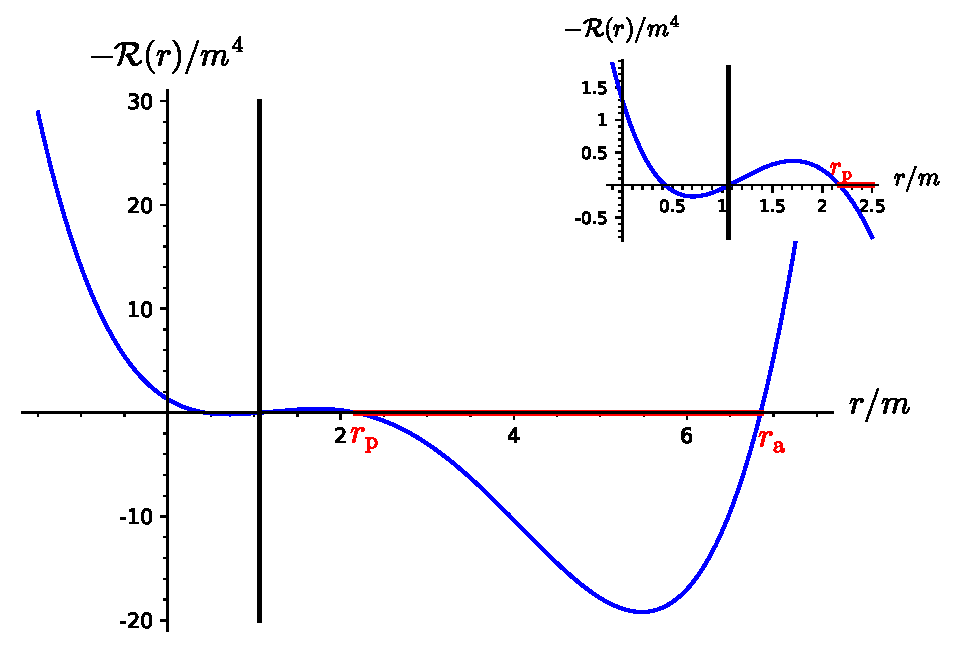
\includegraphics[width=0.7\textwidth]{gek_R_potential.pdf}}
\caption[]{\label{f:gek:R_potential} \footnotesize
Effective potential $-\mathcal{R}(r)$ corresponding to $a=0.998\, m$,
$\veps=0.9$, $\ell=2 m$ and $q=1.3\, m^2$. The black vertical line
marks the black hole horizon at $r=r_+\simeq 1.063\, m$.
Note that the polynomial $-\mathcal{R}(r)$
has four real roots, one of them being very close to, but distinct from, $r_+$.
The two largest roots give the periastron and apoastron of the bound orbit
with the above values of $(\veps,\ell,q)$; they
are respectively $r_p \simeq 2.175\, m$ and
$r_a \simeq 6.853\, m$.
\textsl{[Figure generated by the notebook \ref{s:sam:Kerr_geod_plots}]}
}
\end{figure}

It is clear that the motion in the potential well $U(r) = - \mathcal{R}(r)$
as governed by Eq.~(\ref{e:gek:r_eff_pot_timelike})
(cf. Fig.~\ref{f:gek:R_potential}) is periodic:
\be
    \forall n\in\mathbb{Z},\quad r(\tau' + n \Lambda_r) = r(\tau') ,
\ee
the period
$\Lambda_r$ being the Mino time $\Delta\tau'$ spent to perform a round-trip
between $r_{\rm p}$ and $r_{\rm a}$. By rewriting Eq.~(\ref{e:gek:r_eff_pot_timelike})
as $\D\tau' = \pm \D r / \sqrt{\mathcal{R}(r)}$, we get
\be \label{e:gek:Lambda_r}
    \encadre{ \Lambda_r = 2 \int_{r_{\rm p}}^{r_{\rm a}} \frac{\D r}{\sqrt{\mathcal{R}(r)}} }.
\ee
Since $\mathcal{R}(r)$ is a polynomial of degree 4 [cf. Eq.~(\ref{e:gek:R_timelike})],
the integral in the right-hand side of Eq.~(\ref{e:gek:Lambda_r}) can
be evaluated by means of elliptic integrals. We shall not give the detail
here, referring the interested reader to the article~\cite{FujitH09}.

Regarding the $\th$-motion, we are in the case $L^2 > a^2(E^2 - \mu^2)$
considered in Sec.~\ref{s:gek:th_motion}, since for bound geodesics $E^2 - \mu^2 < 0$.
The effective $\th$-potential $V(\th) = Q - \Theta(\th)$ has then the shape shown in
the left panel of Fig.~\ref{f:gek:th_pot_L_0} for $\ell=0$ and in the left panel
of Fig.~\ref{f:gek:th_pot_L_non0} for $\ell\neq 0$.
We can then distinguish three types of bound orbits:
\begin{itemize}
\item \defin{polar orbit}\index{polar!orbit}: $\Li$ crosses the rotational axis an infinite number
of times; this occurs iff $\ell=0$ and $q > a^2 ( 1-\veps^2)$;
\item \defin{equatorial orbit}\index{equatorial!orbit}: $\Li$ is entirely contained in the
equatorial plane $\th=\pi/2$; for a bound orbit, this occurs iff $q=0$;
\item \defin{non-polar and non-equatorial orbit}\index{non-polar!orbit}: $\Li$ never crosses the rotational axis and oscillates symmetrically about the equatorial plane between
two $\th$-turning points at $\th = \th_{\rm m} \in (0,\pi /2)$ and $\th=\pi-\th_{\rm m}$;
for a bound orbit, this occurs iff $q>0$ and ($\ell\neq 0$ or $q<a^2 ( 1-\veps^2)$).
\end{itemize}
Strictly speaking, there is also the exceptional case $\ell=0$ and
$q = a^2 (1 -\veps^2)$, for which the rotation axis is reached
asymptotically (cf. Sec.~\ref{s:gek:asymptotic_values} and the grey dashed curve
in the left panel of Fig.~\ref{f:gek:th_pot_L_0}).

Circular equatorial orbits will be discussed in Sec.~\ref{s:gek:circ_equat}.
In the following, we focus on non-polar and non-equatorial orbits, which
constitute the generic category of bound timelike orbits.
One has then $\th_{\rm m} \leq \th \leq \pi - \th_{\rm m}$, with $\th_{\rm m}$ given by
Eq.~(\ref{e:gek:th0_E_lt_mu}):
\be \label{e:gek:th_min_arccos}
    \encadre{ \th_{\rm m} = \arccos \sqrt{ \frac{1}{2} \left[ 1 + \frac{\ell^2 + q}{a^2 (1 - \veps^2)}
        - \sqrt{ \left[1 + \frac{\ell^2 + q}{a^2 (1 - \veps^2)}\right] ^2
        - \frac{4q}{a^2 (1 - \veps^2)}} \right] } } ,
\ee
which reduces to Eq.~(\ref{e:gek:th0_L_zero}) for $\ell = 0$:
\be
   \encadre{ \th_{\rm m} = \arccos \sqrt{\frac{q}{a^2 (1 - \veps^2)}} . }_{\, \ell=0}
\ee

From the viewpoint of Eq.~(\ref{e:gek:th_eff_pot_timelike}) above,
non-polar orbits have a periodic $\th$-motion in the potential well $-\tilde{\Theta}(\th)$:
\be
    \forall n\in\mathbb{Z},\quad \th(\tau' + n \Lambda_\th) = \th(\tau') .
\ee
The period
$\Lambda_\theta$ is the Mino time $\Delta\tau'$ spent in a round-trip
between $\th_{\rm m}$ and $\pi-\th_{\rm m}$.
By rewriting Eq.~(\ref{e:gek:th_eff_pot_timelike})
as $\D\tau' = \pm \D \th / \sqrt{\tilde\Theta(\th)}$, we get
\be
    \encadre{ \Lambda_\th = 2 \int_{\th_{\rm m}}^{\pi-\th_{\rm m}}
              \frac{\D \th}{\sqrt{\tilde\Theta(\th)}}
              = 4 \int_{\th_{\rm m}}^{\pi/2}
                  \frac{\D \th}{\sqrt{\tilde\Theta(\th)}} },
\ee
where the last equality results from the symmetry of $\tilde\Theta(\th)$
with respect to $\pi/2$.
One naturally associates to the periods $\Lambda_r$ and $\Lambda_\th$
the \defin{Mino angular frequencies}\index{Mino!angular frequency}\index{angular!frequency!Mino --}:
\be
   \encadre{ \Upsilon_r := \frac{2\pi}{\Lambda_r} }\qquad\mbox{and}\qquad
   \encadre{ \Upsilon_\th := \frac{2\pi}{\Lambda_\th} }.
\ee

\begin{figure}
\centerline{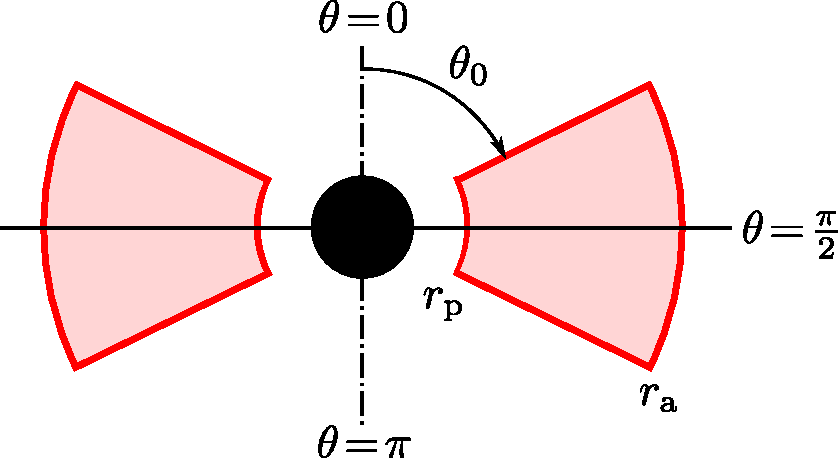
\includegraphics[width=0.5\textwidth]{gek_torus.pdf}}
\caption[]{\label{f:gek:torus} \footnotesize
Meridional section of the torus occupied by a bound timelike geodesic. The dot-dashed line
is the rotation axis and the solid line marks the equatorial plane.
}
\end{figure}

For non-polar orbits, the motion is restricted by
\be
 \encadre{r_{\rm p}\leq r \leq r_{\rm a}} \qquad\mbox{and}\qquad
 \encadre{\th_{\rm m} \leq \th \leq \pi - \th_{\rm m}}.
\ee
This means that in terms of the Cartesian Boyer-Lindquist coordinates (\ref{e:gek:Cartesian_BL}), the
geodesic is confined inside a torus (cf. Fig.~\ref{f:gek:torus}), which is
symmetric about the equatorial plane. Moreover, if the two frequencies
$\Upsilon_r$ and $\Upsilon_\th$ are not commensurable, i.e. if
$\Upsilon_\th / \Upsilon_r \not\in\mathbb{Q}$, the geodesic fills the torus.
Examples of orbits with $\Upsilon_\th / \Upsilon_r \in\mathbb{Q}$, i.e.
orbits with a closed trajectory in the $(r,\th)$ plane, can be
found in Ref.~\cite{GrossLP12}.

\begin{figure}
\centerline{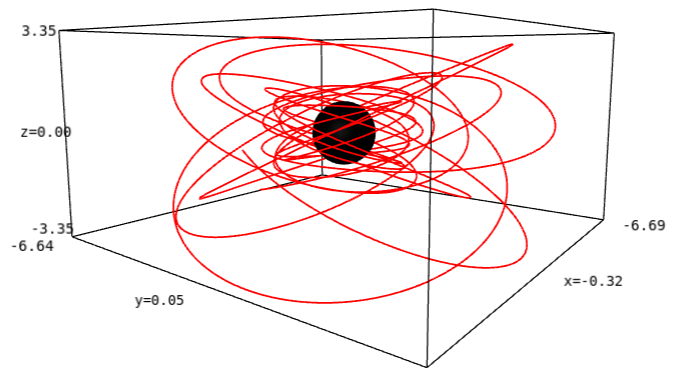
\includegraphics[width=0.7\textwidth]{gek_timelike_xyz.png}}
\caption[]{\label{f:gek:timelike_xyz} \footnotesize
Trajectory with respect to the Cartesian Boyer-Lindquist coordinates
$(x,y,z)$ [Eq.~(\ref{e:gek:Cartesian_BL})]
of a bound timelike geodesic of reduced integrals of motion
$\veps=0.9$, $\ell=2 m$ and $q=1.3\, m^2$, orbiting around a
Kerr black hole with $a=0.998\, m$. These parameters are the same as for
the $-\mathcal{R}(r)$ plot in Fig.~\ref{f:gek:R_potential}.
\textsl{[Figure generated by the notebook \ref{s:sam:Kerr_geod_plots}]}
}
\end{figure}

\begin{figure}
\centerline{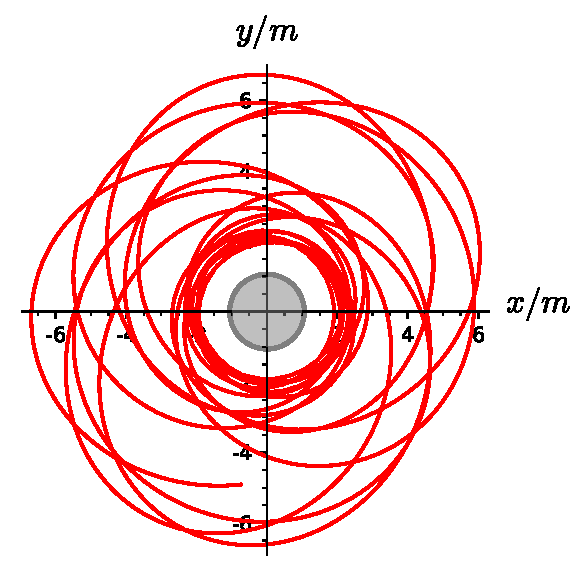
\includegraphics[width=0.42\textwidth]{gek_timelike_xy.pdf}\
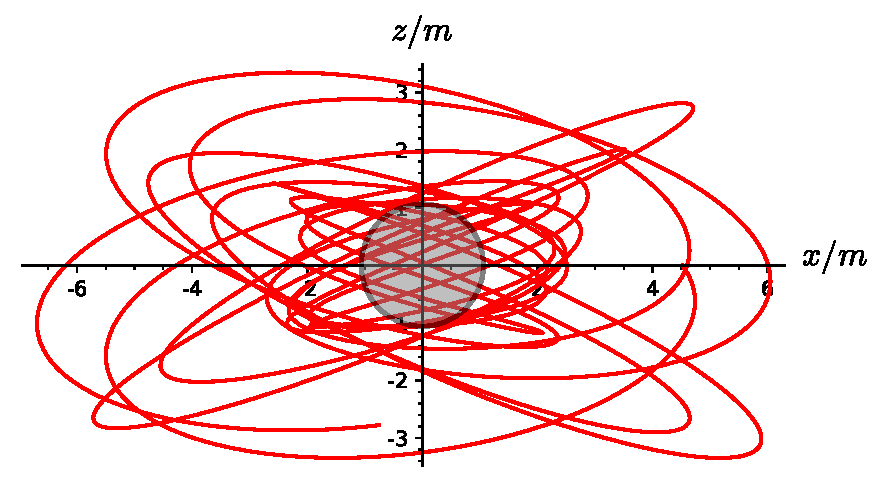
\includegraphics[width=0.55\textwidth]{gek_timelike_xz.pdf}
}
\caption[]{\label{f:gek:timelike_plane} \footnotesize
Projection in the $(x,y)$ plane (equatorial plane; left panel) and the $(x,z)$ plane
(meridional plane; right panel)
of the bound timelike geodesic considered in Fig.~\ref{f:gek:timelike_xyz}.
The grey disk depicts the black hole region. On the left panel, there appears
clearly that the minimal value of $r$ is $r_p \simeq 2.2\, m$, while its
maximal value is $r_a \simeq 6.9\, m$. On the right panel, we check
that $\th_{\rm m} \leq \th \leq \pi -\th_{\rm m}$ with
$\th_{\rm m} \sim 60^\circ$, in agreement with the generic behaviour
illustrated in Fig.~\ref{f:gek:torus}.
\textsl{[Figure generated by the notebook \ref{s:sam:Kerr_geod_plots}]}
}
\end{figure}

\begin{figure}
\centerline{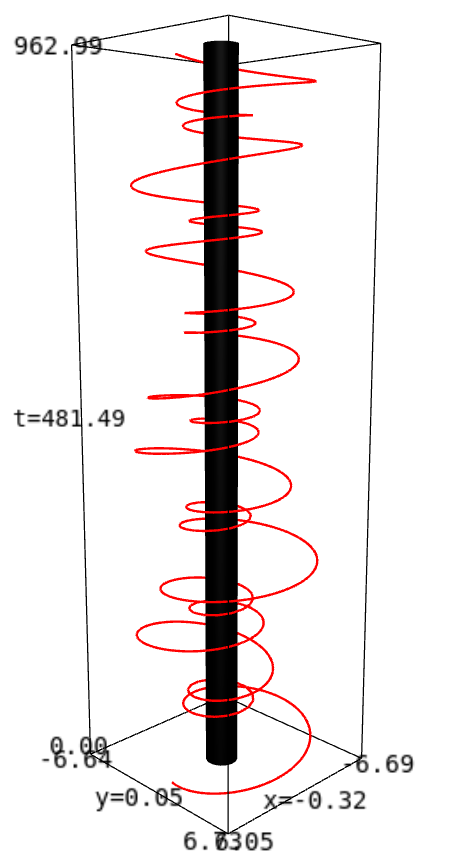
\includegraphics[height=0.4\textheight]{gek_timelike_txy.png}}
\caption[]{\label{f:gek:timelike_txy} \footnotesize
Spacetime diagram based on the Cartesian Boyer-Lindquist coordinates
$(t,x,y)$ [Eq.~(\ref{e:gek:Cartesian_BL})] depicting the bound timelike geodesic
considered in Figs.~\ref{f:gek:timelike_xyz} and \ref{f:gek:timelike_plane}. The black
cylinder is the black hole event horizon.
\textsl{[Figure generated by the notebook \ref{s:sam:Kerr_geod_plots}]}
}
\end{figure}

As an illustration, Figs.~\ref{f:gek:timelike_xyz}--\ref{f:gek:timelike_txy}
show a bound timelike geodesic $\Li$ of reduced integrals of motion
$\veps=0.9$, $\ell=2 m$ and $q=1.3\, m^2$
orbiting around a Kerr black hole with $a=0.998\, m$.
It has $r_p \simeq 2.175\, m$,
$r_a \simeq 6.853\, m$ and $\th_{\rm m} \simeq 1.060\, {\rm rad} \simeq 60.75^\circ$.
The effective radial potential
$-\mathcal{R}(r)$ of this geodesic is the one depicted in Fig.~\ref{f:gek:R_potential}.
Figures~\ref{f:gek:timelike_xyz}--\ref{f:gek:timelike_txy} show actually the
segment $0\leq \tau \leq 600 \, m$ of $\Li$,
starting at the point of Boyer-Lindquist coordinates
$(0, (r_{\rm p} + r_{\rm a})/2, \pi/2, 0)$.
That $\th(\tau)$ lies in the interval
$[\th_{\rm m}, \pi-\th_{\rm m}] \sim [60^\circ, 120^\circ]$ appears clearly in the
right panel of Fig.~\ref{f:gek:timelike_plane}. On Figs.~\ref{f:gek:timelike_plane}
(left panel) and \ref{f:gek:timelike_txy}, we notice a generic feature
of eccentric orbits in the Kerr metric, known as
\defin{zoom-whirl}\index{zoom-whirl}\footnote{According to Ref.~\cite{GlampK02},
the name ``zoom-whirl'' has been forged by Curt Cutler and Eric Poisson and
may have been suggested by Kip Thorne.}:
the particle falls
from its apoastron to the central region (``zoom in'') and performs some
quasi-circular revolutions at close distance to the black hole (it ``whirls''), reaching
the periastron, and finally goes back to the apoastron. The zoom-whirl behaviour
exists as well for eccentric orbits in Schwarzschild spacetime (cf. right panel
of Fig.~\ref{f:ges:orbit_e967_990_l42}), but is less
pronounced, i.e. the number of whirls is smaller (only one in
Fig.~\ref{f:ges:orbit_e967_990_l42}).


Let us now consider the evolution of the coordinates $t$ and $\ph$ along the
geodesic, as governed
by Eqs.~(\ref{e:gek:dtdmino_timelike}) and (\ref{e:gek:dphdmino_timelike}).
Since $r$ and $\th$ are periodic functions of $\tau'$, so are the terms
$T_1(r)$, $T_2(\th)$, $\Phi_1(r)$ and $\Phi_2(\th)$ that appear in the right-hand side
of Eqs.~(\ref{e:gek:dtdmino_timelike}) and (\ref{e:gek:dphdmino_timelike}). We can thus expand them in Fourier series:
\begin{subequations}
\begin{align}
  &  T_1(r) = \sum_{k=-\infty}^{+\infty} \hat{T}_{1k} \, \mathrm{e}^{\mathrm{i} k \Upsilon_r \, \tau'} = \langle T_1(r) \rangle + \sum_{k=1}^{+\infty} \left( \hat{T}_{1k} \, \mathrm{e}^{\mathrm{i} k \Upsilon_r \, \tau'} + \mathrm{c.c.} \right) \\
  &  T_2(\th) = \sum_{k=-\infty}^{+\infty} \hat{T}_{2k} \, \mathrm{e}^{\mathrm{i} k \Upsilon_\th \, \tau'} = \langle T_2(\th) \rangle + \sum_{k=1}^{+\infty} \left( \hat{T}_{2k} \, \mathrm{e}^{\mathrm{i} k \Upsilon_\th \, \tau'} + \mathrm{c.c.} \right) \\
  &  \Phi_1(r) = \sum_{k=-\infty}^{+\infty} \hat{\Phi}_{1k} \, \mathrm{e}^{\mathrm{i} k \Upsilon_r \, \tau'} = \langle \Phi_1(r) \rangle + \sum_{k=1}^{+\infty} \left( \hat{\Phi}_{1k} \, \mathrm{e}^{\mathrm{i} k \Upsilon_r \, \tau'} + \mathrm{c.c.} \right) \\
  &  \Phi_2(\th) = \sum_{k=-\infty}^{+\infty} \hat{\Phi}_{2k} \, \mathrm{e}^{\mathrm{i} k \Upsilon_\th \, \tau'} = \langle \Phi_2(\th) \rangle + \sum_{k=1}^{+\infty} \left( \hat{\Phi}_{2k} \, \mathrm{e}^{\mathrm{i} k \Upsilon_\th \, \tau'} + \mathrm{c.c.} \right) ,
\end{align}
\end{subequations}
where ``c.c.`` stands for \emph{complex conjugate} and $\langle T_1(r) \rangle = \hat{T}_{10}$, $\langle T_2(\th) \rangle = \hat{T}_{20}$,
$\langle \Phi_1(r) \rangle = \hat{\Phi}_{10}$ and $\langle \Phi_2(\th) \rangle = \hat{\Phi}_{20}$
are the mean values of the functions $T_1(r(\tau'))$,
$T_2(\th(\tau'))$, $\Phi_1(r(\tau'))$ and $\Phi_2(\th(\tau'))$ over one period:
\begin{subequations}
\begin{align}
    & \langle T_1(r) \rangle = \frac{1}{\Lambda_r} \int_{0}^{\Lambda_r}
        T_1(r(\tau'))\, \D \tau'
        = \frac{2}{\Lambda_r} \int_{r_{\rm p}}^{r_{\rm a}} \frac{T_1(r)}{\sqrt{R(r)}}\, \D r \\
    & \langle T_2(\th) \rangle = \frac{1}{\Lambda_\th} \int_{0}^{\Lambda_\th}
        T_2(\th(\tau'))\, \D \tau'
        = \frac{4}{\Lambda_\th} \int_{\th_{\rm m}}^{\pi/2}
            \frac{T_2(\th)}{\sqrt{\tilde\Theta(\th)}}\, \D \th ,
\end{align}
\end{subequations}
with similar formulas for $\langle \Phi_1(r) \rangle$ and $\langle \Phi_2(\th) \rangle$.

We may then rewrite Eqs.~(\ref{e:gek:dtdmino_timelike}) and (\ref{e:gek:dphdmino_timelike})
as
\begin{subequations}
\begin{align}
 & \derd{t}{\tau'} = \Gamma + \sum_{k=1}^{+\infty} \left( \hat{T}_{1k} \, \mathrm{e}^{\mathrm{i} k \Upsilon_r \, \tau'} + \mathrm{c.c.} \right)
    + \sum_{k=1}^{+\infty} \left( \hat{T}_{2k} \, \mathrm{e}^{\mathrm{i} k \Upsilon_\th \, \tau'} + \mathrm{c.c.} \right) \\
 & \derd{\ph}{\tau'} = \Upsilon_\ph + \sum_{k=1}^{+\infty} \left( \hat{\Phi}_{1k} \, \mathrm{e}^{\mathrm{i} k \Upsilon_r \, \tau'} + \mathrm{c.c.} \right)
 + \sum_{k=1}^{+\infty} \left( \hat{\Phi}_{2k} \, \mathrm{e}^{\mathrm{i} k \Upsilon_\th \, \tau'} + \mathrm{c.c.} \right) ,
\end{align}
\end{subequations}
with
\be
    \Gamma := \langle T_1(r) \rangle + \langle T_2(\th) \rangle ,
\ee
and
\be
    \Upsilon_\ph :=  \langle \Phi_1(r) \rangle + \langle \Phi_2(\th) \rangle .
\ee
$\Gamma$ and $\Upsilon_\ph$ represent the constant (or average) parts of
respectively $\D t/\D\tau'$ and $\D \ph / \D\tau'$, while the oscillatory parts
are the terms involved in the sums over $k\geq 1$.
Since $\Gamma$ is the average value of $\D t/\D\tau'$,
we can define the
\defin{average angular frequencies with respect to Boyer-Lindquist time}\index{average!angular frequency}
by \cite{DrascH04,FujitH09}
\be
    \Omega_r := \frac{\Upsilon_r}{\Gamma},\qquad
    \Omega_\th := \frac{\Upsilon_\th}{\Gamma}, \qquad
    \Omega_\ph := \frac{\Upsilon_\ph}{\Gamma} .
\ee
We may summarize the above results by
\begin{greybox}
The motion of a generic bound timelike
geodesic in Kerr spacetime is periodic in $r$ and $\th$
only in terms of the Mino time $\tau'$, the corresponding angular frequencies
being $\Upsilon_r$ and $\Upsilon_\th$. In terms of the Boyer-Lindquist time
$t$, the motion in $r$ or $\th$ is not periodic. Accordingly, the ``average
frequencies'' $\Omega_r$ and $\Omega_\th$ defined above are not true
frequencies like $\Upsilon_r$ or $\Upsilon_\th$.
Regarding the motion in $\ph$,
it is not periodic, neither in terms of the Mino time, nor in terms
of the Boyer-Lindquist time, so that both $\Upsilon_\ph$ and $\Omega_\ph$
are average frequencies.
\end{greybox}

\subsubsection{Quasi-Keplerian parametrization}

Given a bound timelike geodesic $\Li$ of Kerr spacetime, one may define
its \defin{eccentricity}\index{eccentricity} $e$ and (dimensionless)
\defin{semilatus rectum} $p$ by means of Keplerian-like formulas \cite{Schmi02,DrascH06,SteinW20}:
\be \label{e:gek:rp_ra_p_e}
    r_{\rm p} =: \frac{p m}{1 + e} \qquad\mbox{and}\qquad
    r_{\rm a} =: \frac{p m}{1 - e} ,
\ee
or equivalently
\be \label{e:gek:p_e_ra_rp}
    p = \frac{2 r_{\rm a} r_{\rm p}}{m (r_{\rm a} + r_{\rm p})}
    \qquad\mbox{and}\qquad
    e = \frac{r_{\rm a} - r_{\rm p}}{r_{\rm a} + r_{\rm p}} .
\ee
One may also introduce the \defin{inclination angle} $\th_{\rm inc}$ by
\be \label{e:gek:def_th_inc}
    \th_{\rm inc} := \frac{\pi}{2} - (\operatorname{sgn}\ell) \th_{\rm m} .
\ee
The sign of $\ell$ appears in this formula to enforce $\th_{\rm inc} \in [0, \pi/2]$
for prograde orbits ($\ell > 0$) and $\th_{\rm inc} \in [\pi/2, \pi]$ for retrograde
orbits ($\ell < 0$).

Instead of $(\veps,\ell,q)$, a bound timelike geodesic
can be parametrized\footnote{Some authors use $x:=\cos\th_{\rm inc}$
instead of $\th_{\rm inc}$ \cite{SteinW20}.}
by $(p, e, \th_{\rm inc})$. Actually, there is a one-to-one
correspondence between $(\veps,\ell,q)$ and $(p, e, \th_{\rm inc})$:
it is clear from formulas (\ref{e:gek:p_e_ra_rp}) and (\ref{e:gek:p_e_ra_rp})
that $(p, e, \th_{\rm inc})$ are functions of $(\veps,\ell,q)$, because
(i) $r_{\rm a}$ and $r_{\rm p}$ are some roots of the quartic polynomial
$\mathcal{R}(r)$, whose coefficients are functions of $(\veps,\ell,q)$ only
(at fixed Kerr parameters $(m, a)$) [cf. Eq.~(\ref{e:gek:R_timelike})] and
(ii) $\th_{\rm m}$ in the right-hand side of expression~(\ref{e:gek:def_th_inc}) for
$\th_{\rm inc}$ is the function of $(\veps,\ell,q)$ given by Eq.~(\ref{e:gek:th_min_arccos}).
Conversely, to express $(\veps,\ell,q)$ in terms of $(p, e, \th_{\rm inc})$,
one shall write
\[
    \left\{ \begin{array}{l}
        \mathcal{R}(r_{\rm p}) = 0 \\
        \mathcal{R}(r_{\rm a}) = 0 \\
        \tilde{\Theta}(\th_{\rm m}) = 0 ,
        \end{array} \right.
\]
where $r_{\rm p}$ and $r_{\rm a}$ are the functions of $(e,p)$ given
by Eq.~(\ref{e:gek:rp_ra_p_e}) and $\th_{\rm m}$ is the function
of $\th_{\rm inc}$ given by Eq.~(\ref{e:gek:def_th_inc}). The above system
is then a system of 3 equations for the 3 unknowns $(\veps,\ell,q)$; see
Appendix~B of Ref.~\cite{Schmi02} or Appendix~A of Ref.~\cite{DrascH06} for details.

\begin{example}
The geodesic $\Li$ depicted in Figs.~\ref{f:gek:timelike_xyz}--\ref{f:gek:timelike_txy}
has $\veps=0.9$, $\ell=2 m$ and $q=1.3\, m^2$, from which we get
$r_p = 2.175\, m$,
$r_a = 6.853\, m$ and $\th_{\rm m} = 1.060\, {\rm rad} = 60.75^\circ$.
Then Eqs.~(\ref{e:gek:p_e_ra_rp}) and (\ref{e:gek:def_th_inc}) yield
$p=3.302$, $e=0.518$ and $\th_{\rm inc} = 29.26^\circ$.
\end{example}

The parametrization $(p, e, \th_{\rm inc})$ allows one to introduce
along the geodesic $\Li$ the radial phase angle $\psi(\tau)$ and the
meridional phase angle $\chi(\tau)$ as monotonically increasing functions
of $\tau$ such that
\be
    r(\tau) =: \frac{p m}{1 + e\cos\psi(\tau)} \qquad\mbox{and}\qquad
    \th(\tau) =: \arccos\left( \cos\th_{\rm m} \, \cos\chi(\tau) \right) .
\ee
For numerical integration, $\psi(\tau)$ and $\chi(\tau)$ are preferred
to $r(\tau)$ and $\th(\tau)$ since the latter are tricky at the
turning points, where $\D r/\D\tau$ and $\D\th/\D\tau$ vanish and change sign
\cite{DrascH04}.

%%%%%%%%%%%%%%%%%%%%%%%%%%%%%%%%%%%%%%%%%%%%%%%%%%%%%%%%%%%%%%%%%%%%%%%%%%%%%%%

\section{Circular timelike orbits in the equatorial plane} \label{s:gek:circ_equat}

\subsection{Equations of motion in the equatorial plane}

Let us focus on timelike geodesics confined to the equatorial plane:
$\th=\pi/2$. They thus have $\D\th/\D\tau' = 0$ and Eq.~(\ref{e:gek:th_eff_pot_timelike})
leads to $\tilde{\Theta}(\th) = 0$. Given expression~(\ref{e:gek:Theta_timelike}) for $\tilde{\Theta}(\th)$, this
implies
\be \label{e:gek_equat_q_zero}
    \encadre{ q = 0 }.
\ee
\begin{remark}
The above result follows as well from the analysis of the $\th$-motion performed
in Sec.~\ref{s:gek:th_motion} and according to which the only possible value of
the Cartan constant $Q$
for a motion confined to the equatorial plane is $Q=0$, be the geodesic timelike or null.
The converse is not true: there exist (timelike or null) geodesics with $Q=0$ outside the equatorial
plane; they are asymptotically approaching the equatorial from one side, except for
the exceptional case $L=0$ and $a^2 E^2 = a^2 \mu^2$, for which they are moving with
a constant value of $\th$ (cf. Sec.~\ref{s:gek:th_motion}).
\end{remark}

When $\th=\pi/2$, we have $\sin^2\th=1$, $\rho^2 = r^2$ and $\D\tau' = r^{-2}\D\tau$
[cf. Eq.~(\ref{e:gek:Mino_time_tau})], so that the system
(\ref{e:gek:timelike_system}) reduces to
\begin{subequations}
\label{e:gek:equat_time_system}
\begin{align}
& \encadre{ \frac{\D t}{\D\tau} = \frac{1}{r^2 - 2 m r + a^2} \left[
    \veps(r^2 + a^2) + \frac{2 a m}{r} (a\veps - \ell) \right] } \label{e:gek:timel_dtdtau} \\
& \encadre{ \left( \frac{\D r}{\D \tau} \right) ^2 + \mathcal{V}(r) = 0 }\label{e:gek:timel_drdtau} \\
& \encadre{ \frac{\D\ph}{\D\tau} = \frac{1}{r^2 - 2 m r + a^2} \left[
    \ell \left( 1 - \frac{2m}{r} \right)
    + \frac{2 am \veps}{r} \right] },  \label{e:gek:timel_dphdtau}
\end{align}
\end{subequations}
with
\be \label{e:gek:def_V_time_equat}
   \encadre{ \mathcal{V}(r) := 1 - \veps^2 - \frac{2m}{r} + \frac{\ell^2 + a^2(1-\veps^2)}{r^2}
    - \frac{2m(\ell - a\veps)^2}{r^3} }.
\ee
Note that $\mathcal{V}(r) = - \mathcal{R}(r)/r^4 = - R(r) / (\mu^2 r^4)$ [cf. Eqs.~(\ref{e:gek:R_timelike}) and (\ref{e:gek:R_r_powers})].
\begin{remark}
At the Schwarzschild limit ($a=0$) we recover the differential equations of Chap.~\ref{s:ges},
namely Eq.~(\ref{e:gek:timel_dtdtau}) reduces to Eq.~(\ref{e:ges:Dt_Dtau}),
Eq.~(\ref{e:gek:timel_drdtau}) to Eq.~(\ref{e:ges:1d_motion_timelike}) and
Eq.~(\ref{e:gek:timel_dphdtau}) to Eq.~(\ref{e:ges:Dph_Dtau}). In particular
we have $\mathcal{V}(r) = 1 - \veps^2 + 2 V_\ell(r)$, where $V_\ell(r)$
is the effective potential (\ref{e:ges:V_eff_timelike}). Note however that
when $a\neq 0$, $\mathcal{V}(r)$ cannot be considered as an effective
potential for the radial motion, because it depends on $\veps$, in addition
to $\ell$, even if we subtract from it the constant term $1 - \veps^2$.
This is why we did not bother to add a $1/2$ factor in Eq.~(\ref{e:gek:timel_drdtau}),
as we did for Eq.~(\ref{e:ges:1d_motion_timelike}) to make it match
the first integral of a 1-dimensional motion in a potential well.
\end{remark}

\subsection{Existence of circular timelike orbits} \label{s:gek:existence_circ_orb}

The simplest equatorial geodesics are of course the circular ones:
a \defin{circular orbit in the equatorial plane}\index{circular!orbit}\index{orbit!circular --}
is a geodesic that obeys
\be \label{e:gek:def_circular_orbit}
    \forall\tau\in\mathbb{R},\quad \theta(\tau) = \pi/2 \qand r(\tau) = r_0 = \mathrm{const} .
\ee
The constant $r_0$ is called the \defin{radius}\index{radius!of circular orbit} of the circular
orbit.
One has then $\D r/\D\tau = 0$, so that Eq.~(\ref{e:gek:timel_drdtau}) implies
\be \label{e:gek:circ_V_zero}
    \encadre{ \mathcal{V}(r_0) = 0 }.
\ee
The above condition is not sufficient to single out a geodesic worldline:
there exist worldlines with constant $r=r_0$ that obey the whole system
(\ref{e:gek:equat_time_system}) (which includes (\ref{e:gek:circ_V_zero}))
but that are not solution of the
geodesic equation (\ref{e:gek:eq_geod})
(see Ref.~\cite{Vanae20} for concrete examples). One must add a second condition, which
is obtained as follows. For any timelike equatorial geodesic (not necessarily
circular), the following relation must hold:
\[
    \derd{r}{\tau} \left[ 2 \dderd{r}{\tau} + \mathcal{V}'(r) \right] = 0 .
\]
It is obtained by differentiating Eq.~(\ref{e:gek:timel_drdtau}) with respect
to $\tau$. If the geodesic is not circular, at any point where $r$ is not
stationary (i.e. excluding $r$-turning points), we have $\D r/\D\tau \neq 0$
and the above relation implies
\[
    \mathcal{V}'(r) = - 2 \dderd{r}{\tau} .
\]
Since in the vicinity of any circular geodesic there exist non-circular ones
(those with small eccentricity $e$, as defined by Eq.~(\ref{e:gek:p_e_ra_rp})), by continuity, we shall ask that this relation
holds for circular geodesics as well. For the latter ones, $r=r_0$ and
$\D^2 r/\D\tau^2 = 0$, so that it simplifies to
\be \label{e:gek:circ_derV_zero}
    \encadre{\mathcal{V}'(r_0) = 0 }.
\ee
One can verify\footnote{See Ref.~\cite{Vanae20} for details.} that this
relation, in conjunction with Eq.~(\ref{e:gek:circ_V_zero}), is sufficient
to eliminate the non-geodesic circular worldlines.

To summarize, circular timelike geodesics in the equatorial plane are
obtained by solving the system (\ref{e:gek:circ_V_zero})-(\ref{e:gek:circ_derV_zero}).
Given expression (\ref{e:gek:def_V_time_equat}) for $\mathcal{V}$, this
system takes the form
\begin{subnumcases}{\label{e:gek:syst_r0_eps_ell}}
(1 - \veps^2) r_0^3  - 2 m r_0^2 + \left[ \ell^2 + a^2 (1-\veps^2) \right] r_0
    - 2m (\ell - a\veps)^2 = 0  \\
m r_0^2 - \left[ \ell^2 + a^2 (1-\veps^2) \right] r_0 + 3 m (\ell - a\veps)^2 = 0
        \label{e:gek:syst_r0_eps_ell_2}.
\end{subnumcases}
This is a system of 2 nonlinear equations for 3 unknowns: $r_0$, $\veps$ and $\ell$.
We thus expect a 1-parameter family of solutions. It is convenient to choose
$r_0$ as the parameter. We have thus to solve (\ref{e:gek:syst_r0_eps_ell})
for $(\veps,\ell)$. The change of variable
\be \label{e:gek:def_tilde_l}
    \tilde{\ell} := \ell - a \veps
\ee
turns (\ref{e:gek:syst_r0_eps_ell}) into the system
\begin{subnumcases}{}
r_0^3 \veps^2 =  m \tilde{\ell}^2 + r_0^2 (r_0 - m) \label{e:gek:r03_eps2} \\
2 a r_0 \, \veps\tilde{\ell} = (3m - r_0) \tilde{\ell}^2 + r_0 ( m r_0 - a^2) . \label{e:gek:ar0_eps_ell}
\end{subnumcases}
Let us consider the square of Eq.~(\ref{e:gek:ar0_eps_ell}):
\be \label{e:gek:ar0_eps_ell_square}
    4 a^2 r_0^2\,  \veps^2 \tilde{\ell}^2 = \left[ (3m - r_0) \tilde{\ell}^2 + r_0 ( m r_0 - a^2) \right] ^2 ,
\ee
and substitute (\ref{e:gek:r03_eps2}) for $\veps^2$ in it; we get
\[
    \left[ r_0 (r_0 - 3m)^2  - 4 a^2 m \right] \tilde{\ell}^4
    + 2 r_0^2 \left[ (3 m^2 - a^2) r_0 - m (r_0^2 + a^2)\right] \tilde{\ell}^2
        + r_0^3 (m r_0 - a^2)^2 = 0 .
\]
This is a quadratic equation for $X:=\tilde{\ell}^2$. Its discriminant turns out to
have a simple form:
\[
 \mathit{\Delta} = 16 a^2 m r_0^3 (r_0^2 - 2m r_0 + a^2)^2 .
\]
It follows immediately that $\mathit{\Delta} \geq 0 \iff r_0 \geq 0$. Hence, there is
no solution for $r_0 < 0$:
\begin{greybox}
There does not exist any equatorial circular timelike orbit in the region $r<0$ of
Kerr spacetime.
\end{greybox}
\begin{remark}
For $r_0 < 0$ with $|r_0|\gg m$, the above result is not surprising since we
have seen in Sec.~\ref{s:ker:basic_prop} that under these conditions,
the Kerr metric appears as a Schwarzschild metric with a negative mass. The
asymptotic gravitational field is then repulsive and certainly does not admit
any circular orbit. In the region $r < 0$ and $|r|$ small, the above argument does not apply.
However, the results obtained in Sec.~\ref{s:gek:r-motion}
show that if a circular orbit would exist there, it would necessarily
have $|E| > \mu$ [cf. Eq.~(\ref{e:ker:neg_r_large_E})], i.e. would be unbound.
\end{remark}
The case $r_0=0$ is excluded as well, since in the equatorial plane, it would
correspond to the curvature singularity. In what follows, we therefore assume
\be \label{e:gek:circ_r0_positive}
    \encadre{ r_0 > 0 }.
\ee
We have then $\sqrt{\mathit{\Delta}} = 4 a r_0 \sqrt{m r_0} |r_0^2 - 2m r_0 + a^2|$
and the solutions of the quadratic equation are\footnote{For future convenience, we have
chosen the sign $\mp$ in the numerator to be the opposite of the label $\pm$
in $\tilde{\ell}^2_{\pm}$.}
\be \label{e:gek:sol_tell2}
    \tilde{\ell}^2_{\pm} = r_0 \frac{ (a^2 - 3m^2) r_0^2 + m r_0 (r_0^2 + a^2)
    \mp 2 a \sqrt{m r_0} (r_0^2 - 2m r_0 + a^2)}{r_0 (r_0 - 3m)^2  - 4 a^2 m} .
\ee
The denominator of the right-hand side can be written as
\[
    r_0 (r_0 - 3m)^2  - 4 a^2 m = \frac{1}{r_0} \left[
        \left( r_0 (r_0 - 3m) \right) ^2 - \left( 2 a \sqrt{m r_0} \right) ^2 \right]
        = \frac{1}{r_0} A_+ A_- ,
\]
with
\[
    A_\pm := r_0 (r_0 - 3m) \pm 2 a \sqrt{m r_0} .
\]
In the numerator of (\ref{e:gek:sol_tell2}), we may use the identity
$\mp 2 a \sqrt{m r_0} = A_\mp - r_0 (r_0 - 3m)$ and get, after
simplification,
\[
    \tilde{\ell}^2_{\pm} = \frac{r_0^2}{A_+ A_-} \left[ A_\mp (r_0^2 - 2m r_0 + a^2)
     - A_+ A_- \right] = \frac{r_0^2}{A_\pm} \left(
        r_0^2 - 2m r_0 + a^2 - A_\pm \right) .
\]
Using $r_0^2 - 2m r_0 + a^2 - A_\pm  =  a^2 \mp 2a \sqrt{m r_0} + m r_0 =
(a \mp \sqrt{m r_0})^2$, we obtain
\be \label{e:gek:tell2_circ}
    \tilde{\ell}^2_{\pm} = \frac{r_0^2 (a \mp \sqrt{m r_0})^2}{r_0^2 - 3m r_0 \pm 2 a \sqrt{m r_0}} .
\ee
Since obviously $\tilde{\ell}^2_{\pm} \geq 0$, this expression gives birth to
the constraint $r_0^2 - 3m r_0 \pm 2 a \sqrt{m r_0} > 0$,
which is equivalent to
\be \label{e:gek:cubic_sqrt_r0}
    r_0^{3/2} - 3 m r_0^{1/2}  \pm 2 a \sqrt{m} > 0 .
\ee
The left hand-side of this inequality is a cubic polynomial in $x:=r_0^{1/2}$
and determining its sign amounts to compute its roots. Fortunately, this
corresponds to
a depressed cubic equation $x^3 + px + q = 0$, with $p:= -3m$ and $q:=\pm 2 a \sqrt{m}$,
the discriminant of which is $-(4 p^3 + 27 q^2) = 108 m (m^2 - a^2) \geq 0$. The roots
$(x_k)_{k\in\{0,1,2\}}$ are then all real and are given by Viète's formula (\ref{e:gis:Viete}).
They obey $x_0 + x_1 + x_2 = 0$ and $x_0 x_1 x_2 = -q = \mp 2 a \sqrt{m}$,
from which we deduce that for $\pm = +$ in Eq.~(\ref{e:gek:cubic_sqrt_r0}), i.e. for
$\tilde{\ell}^2_+$, there are two positive roots, which are $x_0$ and $x_2$
as given by Eq.~(\ref{e:gis:Viete}), while for $\pm = -$, i.e. for
$\tilde{\ell}^2_-$, there is a single positive root, which is $x_0$ as
given by Eq.~(\ref{e:gis:Viete}).
Going back to $r_0 = x^2$, with the roots $x_0$ and $x_2$ given by
Viète's formula (\ref{e:gis:Viete}), we get the following constraints
for circular orbits in the equatorial plane:
\begin{subequations}
\label{e:gek:range_circ}
\begin{align}
    & \mbox{for}\ \tilde{\ell}^2_+:\qquad
    0 < r_0 < r_{\rm ph}^* \qquad\mbox{or}\qquad r_0 > r_{\rm ph}^+ \label{e:gek:range_circ_plus} \\
    & \mbox{for}\ \tilde{\ell}^2_-:\qquad r_0 > r_{\rm ph}^- , \label{e:gek:range_circ_minus}
\end{align}
\end{subequations}
with
\be \label{e:gek:def_r_min_pm}
   \encadre{ r_{\rm ph}^\pm := 4m\cos^2 \left[ \frac{1}{3} \arccos\left( \mp \frac{a}{m} \right) \right] }
\ee
and
\be \label{e:gek:def_r_star}
   \encadre{ r_{\rm ph}^* := 4m\cos^2 \left[ \frac{1}{3} \arccos\left(-\frac{a}{m} \right)  + \frac{4\pi}{3} \right] } .
\ee
The index ``ph'' stands for \emph{photon}, because we shall see in Sec.~\ref{s:gek:circ_velocities}
and in Sec.~\ref{s:gik:spherical_orbits} that these radii actually correspond to
photon orbits (circular null geodesics).
$r_{\rm ph}^\pm$ and $r_{\rm ph}^*$ are plotted as functions of $a$ in Fig.~\ref{f:gek:circ_orb_lim}
(green curves).
Note that $m\leq r_{\rm ph}^+ \leq 3 m$ and $3m \leq r_{\rm ph}^- \leq 4m$,
with
\be \label{e:gek:lim_rph_pm}
    \lim_{a\to 0} r_{\rm ph}^\pm = 3m, \quad
    \lim_{a\to m} r_{\rm ph}^+ = m, \quad
    \lim_{a\to m} r_{\rm ph}^- = 4 m .
\ee
Besides, $0 \leq r_{\rm ph}^* \leq m$, with
\be \label{e:gek:lim_rph_s}
    \lim_{a\to 0} r_{\rm ph}^* = 0, \quad
    \lim_{a\to m} r_{\rm ph}^* = m .
\ee
Furthermore, one can check that
\be
    r_{\rm ph}^\pm \geq r_+
\ee
and
\be \label{e:gek:rs_range}
    0 \leq r_{\rm ph}^* \leq r_- ,
\ee
where $r_+ := m^2 - \sqrt{m^2 - a^2}$ and $r_- := m^2 - \sqrt{m^2 - a^2}$ [Eq.~(\ref{e:ker:def_r_pm})]
are the radii of respectively the event horizon $\Hor$ and the inner horizon $\Hor_{\rm in}$.
Regarding the upper bound in Eq.~(\ref{e:gek:rs_range}), one can see from Fig.~\ref{f:gek:circ_orb_lim} that $r_{\rm ph}^*$ is always very close to $r_-$. The maximum discrepancy is
$r_- - r_{\rm ph}^* \simeq  0.032 \, m$ and is achieved for $a\simeq 0.9 \, m$
(cf. the notebook \ref{s:sam:Kerr_circular_orbits}).
We conclude that the first permitted range for circular orbits in (\ref{e:gek:range_circ_plus}) lies
entirely in the region $\M_{\rm III}$ of Kerr spacetime, while the second range
in (\ref{e:gek:range_circ_plus}) lies in entirely in $\M_{\rm I}$. Regarding
the orbits for $\tilde{\ell}^2_-$, the range (\ref{e:gek:range_circ_minus}) lies in $\M_{\rm I}$
as well.

\begin{figure}
\centerline{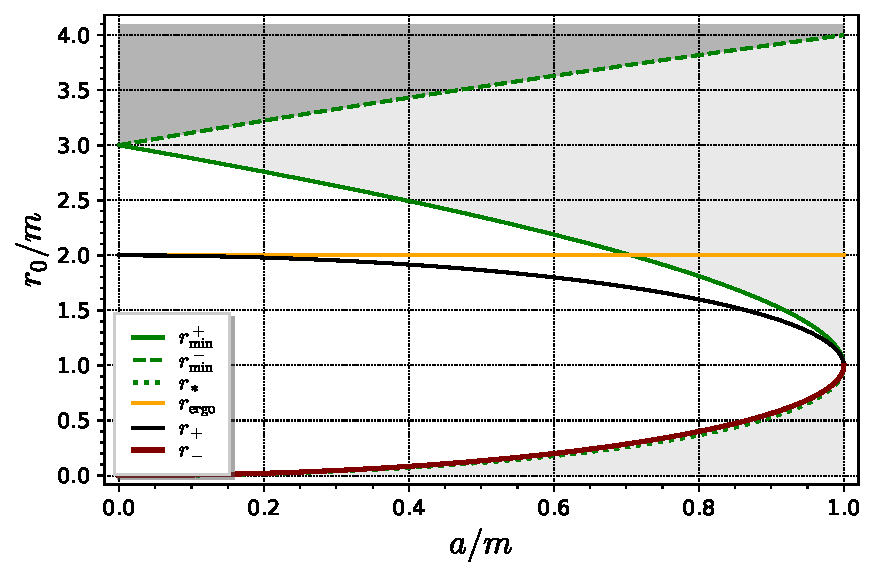
\includegraphics[width=0.7\textwidth]{gek_circ_orb_lim.pdf}}
\caption[]{\label{f:gek:circ_orb_lim} \footnotesize
Domain of existence of circular equatorial timelike orbits in the $(a, r_0)$ plane:
orbits of the $(\veps_+,\ell_+)$ family exist in both the light and dark grey regions,
while orbits of the $(\veps_-,\ell_-)$ family exist only in the dark grey region.
The orange line marks
the location of the outer ergosphere in the equatorial plane, which is
$r_{\rm ergo} = r_{\E^+}(\pi/2) = 2m$ [cf. Eq.~(\ref{e:ker:r_ergo_p_eq})],
the black curve corresponds to the black hole event horizon $\Hor$
($r=r_+$) and the maroon one to the inner horizon
$\Hor_{\rm in}$ ($r=r_-$).
\textsl{[Figure generated by the notebook \ref{s:sam:Kerr_circular_orbits}]}
}
\end{figure}



Substituting expression (\ref{e:gek:tell2_circ})
for $\tilde{\ell}^2$ in Eq.~(\ref{e:gek:r03_eps2}), we get,
after simplification,
\be \label{e:gek:eps2_circ}
    \veps^2_{\pm} = \frac{\left( r_0^2 -2m r_0 \pm a \sqrt{mr_0} \right) ^2}{r_0^2\left(r_0^2 - 3m r_0 \pm 2 a \sqrt{m r_0}\right)} .
\ee
The $\pm$'s in Eqs.~(\ref{e:gek:tell2_circ}) and (\ref{e:gek:eps2_circ}) have
to be consistent. In other words, we have two pairs of solutions for
$(\veps^2, \tilde{\ell}^2)$, namely $(\veps_+^2, \tilde{\ell}_+^2)$
and $(\veps_-^2, \tilde{\ell}_-^2)$.
A priori, $\veps_+^2$ leads to two values for $\veps$, namely $\pm\sqrt{\veps_+^2}$,
and $\tilde{\ell}_+^2$ leads to two values for $\tilde{\ell}$, namely $\pm\sqrt{\tilde{\ell}_+^2}$,
so that the pair $(\veps_+^2, \tilde{\ell}_+^2)$ would generate four solutions
for $(\veps, \tilde{\ell})$, and similarly the pair $(\veps_-^2, \tilde{\ell}_-^2)$ would generate four extra solutions for $(\veps, \tilde{\ell})$, leading to a total of eight solutions.
However, by construction these solutions satisfy the ``squared'' equation (\ref{e:gek:ar0_eps_ell_square})
but not all of them satisfy the original equation (\ref{e:gek:ar0_eps_ell}).
To see this, let us consider the following square roots of Eqs.~(\ref{e:gek:eps2_circ})
and (\ref{e:gek:tell2_circ}):
\be \label{e:gek:veps_circ}
    \encadre{ \veps_{\pm} = \frac{r_0^2 -2m r_0 \pm a \sqrt{mr_0}}{r_0\sqrt{r_0^2 - 3m r_0 \pm 2 a \sqrt{m r_0}}} },
\ee
\be \label{e:gek:tell_circ}
    \tilde{\ell}_{\pm} = - \frac{r_0 (a \mp \sqrt{m r_0})}{\sqrt{r_0^2 - 3m r_0 \pm 2 a \sqrt{m r_0}}} = \frac{r_0 (\pm \sqrt{m r_0} - a)}{\sqrt{r_0^2 - 3m r_0 \pm 2 a \sqrt{m r_0}}}
\ee
and write the eight solutions of (\ref{e:gek:ar0_eps_ell_square}) as
\[
    (\veps, \tilde{\ell}) = \left( \epsilon_1 \veps_\pm, \epsilon_2 \tilde{\ell}_\pm \right) ,
    \qquad\mbox{with}\quad \epsilon_1 = \pm 1\qand \epsilon_2 = \pm 1.
\]
By a direct calculation, we get
\[
    2 a r_0 \, \veps\tilde{\ell} - (3m - r_0) \tilde{\ell}^2 - r_0 ( m r_0 - a^2)
    =  \frac{2(1 - \epsilon_1 \epsilon_2) a r_0 (a \mp \sqrt{m r_0}) (r_0^2 - 2m r_0 \pm a\sqrt{m r_0})}{r_0^2 - 3m r_0 \pm 2 a \sqrt{m r_0}} .
\]
Hence Eq.~(\ref{e:gek:ar0_eps_ell}) is fulfilled iff $ 1 - \epsilon_1 \epsilon_2 = 0$, i.e.
iff $\epsilon_1 \epsilon_2 = 1$.
This reduces the number of possible solutions from eight to four:
\be \label{e:gek:circ_four_sol}
    (\veps, \tilde{\ell}) = (\veps_+, \tilde{\ell}_+)\quad\mbox{or}\quad
        (-\veps_+, -\tilde{\ell}_+)\quad\mbox{or}\quad
        (\veps_-, \tilde{\ell}_-)\quad\mbox{or}\quad  (-\veps_-, -\tilde{\ell}_-) .
\ee
A further reduction of the number of solutions is provided by the future-directed condition (\ref{e:gek:future_directed}).
Since $R(r_0) = -\mu^2 r_0^4 \mathcal{V}(r_0) = 0$ by virtue of Eq.~(\ref{e:gek:circ_V_zero}),
for circular equatorial orbits, Eq.~(\ref{e:gek:future_directed}) reduces to
\[
\frac{1}{\Delta_0} \left( \veps - \frac{a}{r_0^2 + a^2} \ell \right) > 0 ,
\]
where $\Delta_0 := r_0^2 - 2 m r_0 + a^2 = (r_0 - r_+)(r_0 - r_-)$. Now, we have
observed above that circular orbits lie either in $\M_{\rm I}$ or $\M_{\rm III}$,
where $\Delta_0 > 0$. Therefore, we can further simplify the future-directed condition to
\[
   \veps - \frac{a}{r_0^2 + a^2} \ell > 0 .
\]
Once reexpressed in terms of $\tilde{\ell} = \ell - a \veps$, it is equivalent to
\be
    r_0^2 \veps - a \tilde{\ell}  >  0 .
\ee
Let us check each of the four solutions (\ref{e:gek:circ_four_sol}):
\begin{align}
  & r_0^2 \veps_+ - a \tilde{\ell}_+ = \frac{r_0 \Delta_0}{\sqrt{r_0^2 - 3m r_0 + 2 a \sqrt{m r_0}}} > 0 \nonumber \\
  & r_0^2 (-\veps_+) - a (-\tilde{\ell}_+) = - (r_0^2 \veps_+ - a \tilde{\ell}_+) < 0 \nonumber \\
  & r_0^2 \veps_- - a \tilde{\ell}_- = \frac{r_0 \Delta_0}{\sqrt{r_0^2 - 3m r_0 - 2 a \sqrt{m r_0}}} > 0 \nonumber \\
  & r_0^2 (-\veps_-) - a (-\tilde{\ell}_-) = - ( r_0^2 \veps_- - a \tilde{\ell}_- ) < 0 . \nonumber
\end{align}
We conclude that only two solutions remain:
\be
    (\veps, \tilde{\ell}) = (\veps_+, \tilde{\ell}_+)\quad\mbox{or}\quad
        (\veps_-, \tilde{\ell}_-) .
\ee
\begin{figure}
\begin{center}
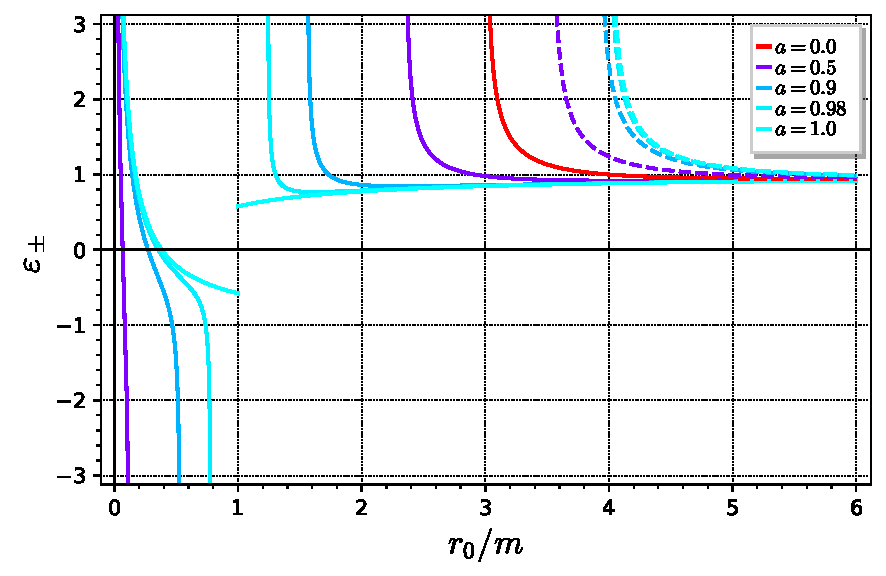
\includegraphics[width=0.65\textwidth]{gek_eps_circ_orb.pdf}\\
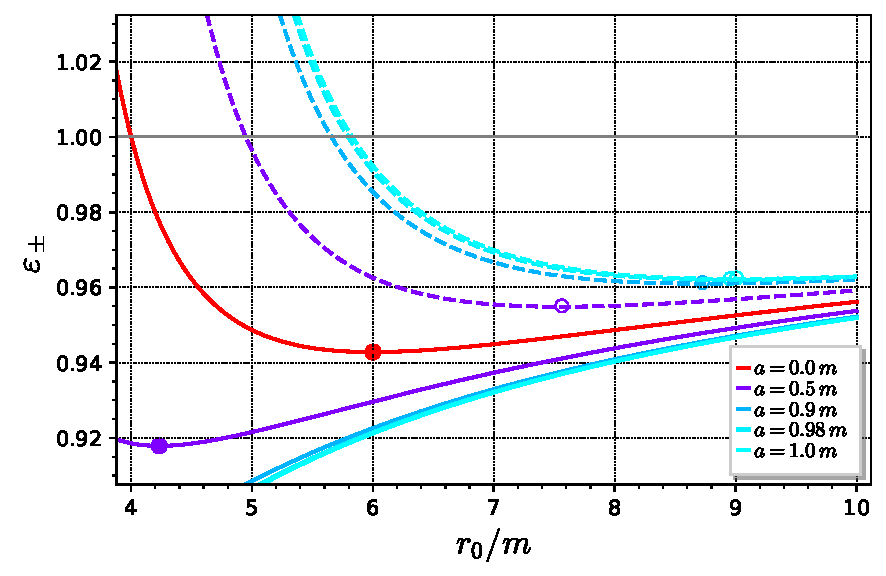
\includegraphics[width=0.65\textwidth]{gek_eps_circ_orb_zoom.pdf}
\end{center}
\caption[]{\label{f:gek:eps_circ_orb} \footnotesize
Specific conserved energy $\veps=\veps_+$ (solid curves) or $\veps=\veps_-$
(dashed curves) along circular timelike
orbits in the equatorial plane, as a function of the orbital radius $r_0$
[Eq.~(\ref{e:gek:veps_circ})], for selected values of the Kerr spin parameter $a$.
Curves in the inner region ($r_0 < m$) terminate by a vertical asymptote at $r = r_{\rm ph}^*(a)$ given
by Eq.~(\ref{e:gek:def_r_star}), while the other curves start along a
vertical asymptote at $r = r_{\rm ph}^\pm(a)$ given by Eq.~(\ref{e:gek:def_r_min_pm}).
Dots on $\veps_+$ curves and open circles on $\veps_-$ ones mark the ISCO: all
configurations on the left of these points are unstable.
The bottom panel is a zoom on the region $4\,m \leq r_0 \leq 10\,m$.
Note that the red curve ($a=0$) is the same as in Fig.~\ref{f:ges:ener_circ_orbit}.
\textsl{[Figure generated by the notebook \ref{s:sam:Kerr_circular_orbits}]}
}
\end{figure}
Given that $\ell = \tilde{\ell} + a \veps$ [Eq.~(\ref{e:gek:def_tilde_l})]
and expressions (\ref{e:gek:veps_circ}) and (\ref{e:gek:tell_circ}) for respectively
$\veps_\pm$ and $\tilde{\ell}_\pm$, these two solutions
can be reexpressed in terms of $(\veps,\ell)$ as
\be \label{e:gek:circ_two_sol}
    (\veps, \ell) = \encadre{ (\veps_+, \ell_+)}\quad\mbox{or}\quad
    \encadre{(\veps_-, \ell_-)} ,
\ee
where
\be \label{e:gek:ell_circ}
    \encadre{ \ell_\pm = \pm \sqrt{\frac{m}{r_0}}
    \frac{r_0^2 + a^2 \mp 2 a \sqrt{mr_0}}{\sqrt{r_0^2 - 3m r_0 \pm 2 a \sqrt{m r_0}}} } .
\ee
The quantities $\veps_\pm$ and $\ell_\pm$ are plotted in terms of $r_0$ in
Figs.~\ref{f:gek:eps_circ_orb} and \ref{f:gek:ell_circ_orb}.
\begin{figure}
\begin{center}
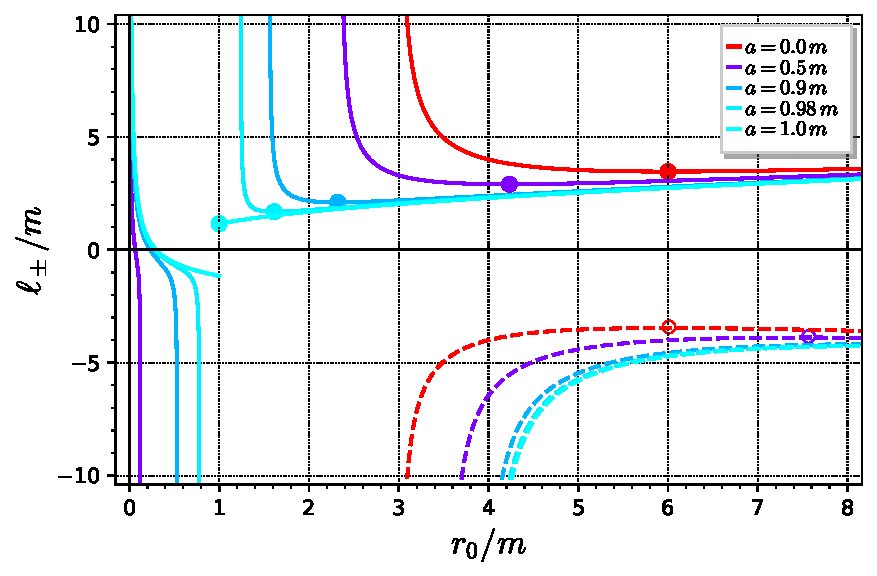
\includegraphics[width=0.65\textwidth]{gek_ell_circ_orb.pdf}\\
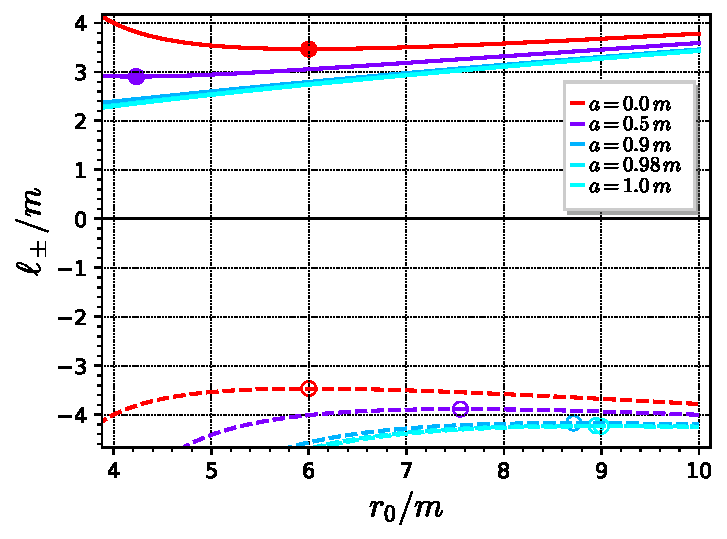
\includegraphics[width=0.65\textwidth]{gek_ell_circ_orb_zoom.pdf}
\end{center}
\caption[]{\label{f:gek:ell_circ_orb} \footnotesize
Specific conserved angular momentum $\ell=\ell_+$ (solid curves) or $\ell=\ell_-$
(dashed curves) along circular timelike
orbits in the equatorial plane, as a function of the orbital radius $r_0$
[Eq.~(\ref{e:gek:ell_circ})], for selected values of the Kerr spin parameter $a$.
Curves in the inner region ($r_0 < m$) terminate by a vertical asymptote at $r = r_{\rm ph}^*(a)$ given
by Eq.~(\ref{e:gek:def_r_star}), while the other curves start along a
vertical asymptote at $r = r_{\rm ph}^\pm(a)$ given by Eq.~(\ref{e:gek:def_r_min_pm}).
Dots on $\ell_+$ curves and open circles on $\ell_-$ ones mark the ISCO: all
configurations on the left of these points are unstable.
The bottom panel is a zoom on the region $4\,m \leq r_0 \leq 10\,m$.
\textsl{[Figure generated by the notebook \ref{s:sam:Kerr_circular_orbits}]}
}
\end{figure}
Orbits with $\ell > 0$ (resp. $\ell < 0$) are called \defin{prograde}\index{prograde!orbit}
(resp. \defin{retrograde}\index{retrograde!orbit}).
We have immediately $\ell_- < 0$, while the sign of $\ell_+$ is that of
of $r_0^2 + a^2 - 2 a \sqrt{mr_0}$.
Outside the event horizon, i.e. in $\M_{\rm I}$, we have $r_0 > m$, which
implies $r_0^2 + a^2 - 2 a \sqrt{mr_0} > r_0^2 + a^2 - 2 a r_0 = (r_0 - a)^2 > 0$. Hence
\be
    r_0 > r_{\rm ph}^+ \quad\Longrightarrow\quad \ell_+ > 0 .
\ee
But for $r_0 < r_{\rm ph}^*$, i.e. in region $\M_{\rm III}$, we may have $\ell_+ < 0$
(cf. Fig.~\ref{f:gek:ell_circ_orb}).
In view of this and the result (\ref{e:gek:range_circ}), we introduce the following nomenclature:
\begin{itemize}
\item orbits of the $(\veps_+,\ell_+)$ family with $r_0 >  r_{\rm ph}^+$
are called \defin{prograde outer circular orbits}\index{prograde!outer circular!timelike orbit};
\item orbits of the $(\veps_+,\ell_+)$ family with $0 < r_0 < r_{\rm ph}^*$
are called \defin{inner circular orbits}\index{inner!circular!timelike orbit};
\item all orbits of the $(\veps_-,\ell_-)$ family
are called \defin{retrograde outer circular orbits}\index{retrograde!outer circular!timelike orbit}.
\end{itemize}

We note from Figs.~\ref{f:gek:eps_circ_orb} and \ref{f:gek:ell_circ_orb},
or from formulas (\ref{e:gek:veps_circ}) and (\ref{e:gek:ell_circ}),
that both $\veps$ and $\ell$ are diverging at the boundaries of the various domains
of existence of circular orbits. We shall comment further on this behaviour at the end of
Sec.~\ref{s:gek:circ_velocities}.

Figure~\ref{f:gek:ell_eps_circ_orb} shows $\veps$ in terms of $\ell$
for the three families of circular orbits, with the indication of
the stability of the various
branches, as determined in the next section.

\begin{figure}
\centerline{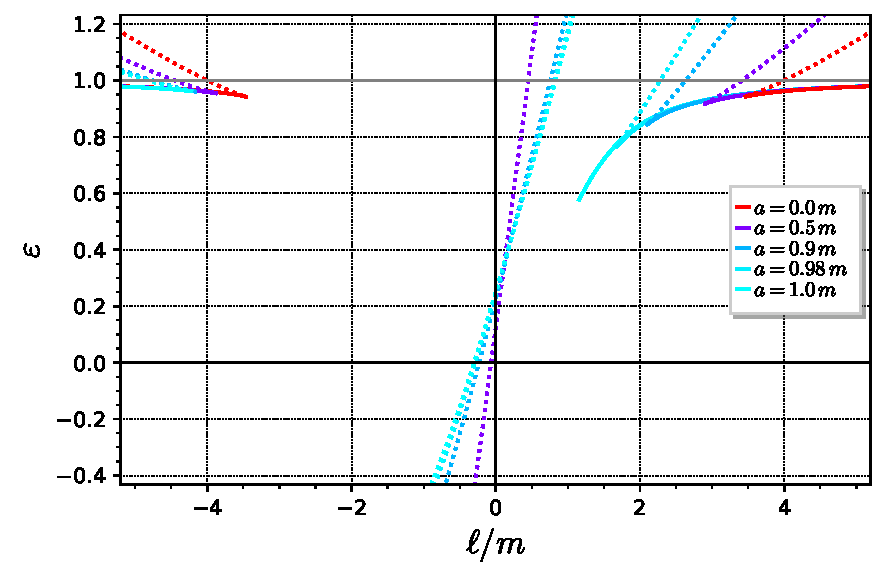
\includegraphics[width=0.7\textwidth]{gek_ell_eps_circ_orb.pdf}}
\caption[]{\label{f:gek:ell_eps_circ_orb} \footnotesize
Circular timelike orbits in the $(\ell,\veps)$ plane, $\ell$ being the
specific conserved angular momentum and $\veps$ the specific conserved
energy. Solid (resp. dotted) curves correspond to stable (unstable) orbits.
Retrograde outer circular orbits are on the left side, inner circular orbits
in the middle and prograde outer circular orbits on the right side.
The cusps in the left and right curves correspond to ISCOs.
\textsl{[Figure generated by the notebook \ref{s:sam:Kerr_circular_orbits}]}
}
\end{figure}



\begin{figure}
\centerline{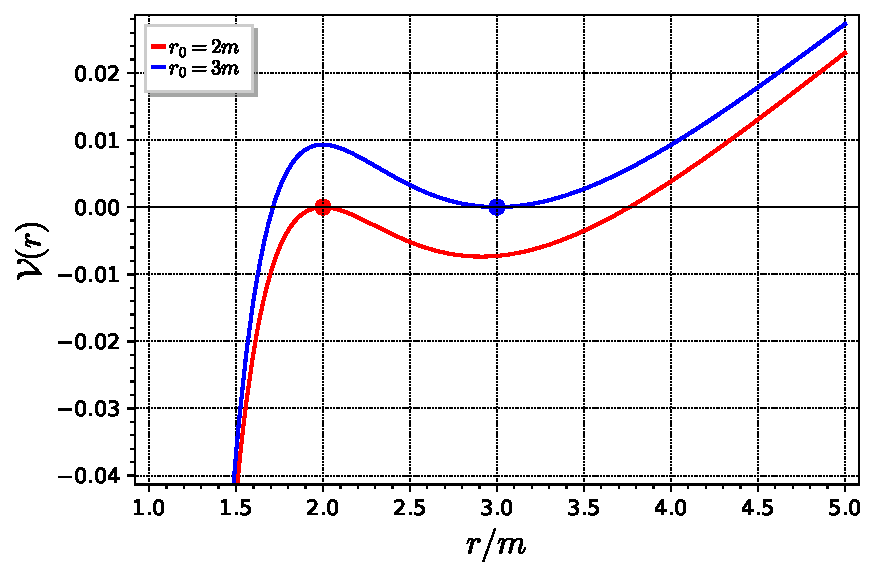
\includegraphics[width=0.7\textwidth]{gek_V_stability.pdf}}
\caption[]{\label{f:gek:V_stability} \footnotesize
Function $\mathcal{V}(r)$, as defined by Eq.~(\ref{e:gek:def_V_time_equat}),
with $a=0.9\, m$, $\veps = \veps_+(r_0)$ [Eq.~(\ref{e:gek:veps_circ})],
$\ell = \ell_+(r_0)$ [Eq.~(\ref{e:gek:ell_circ})] for $r_0 = 2\, m$
(red curve) and $r_0 = 3 \, m$ (blue curve). By definition of $\veps_+$ and $\ell_+$,
one has both $\mathcal{V}(r_0) = 0$ and $\mathcal{V}'(r_0) = 0$.
\textsl{[Figure generated by the notebook \ref{s:sam:Kerr_circular_orbits}]}
}
\end{figure}



\subsection{Stability of circular timelike orbits} \label{s:gek:circ_orb_stab}

\subsubsection{Latitudinal stability}

A natural question regarding the stability of equatorial circular orbits
is whether these orbits are stably confined into the equatorial plane
$\th=\pi/2$. The answer is very simple:
\begin{greybox}
All circular timelike orbits are stable with respect to any perturbation
away from the equatorial plane.
\end{greybox}
\begin{proof}
All equatorial orbits have a vanishing Carter constant $Q$
[cf. Eq.~(\ref{e:gek_equat_q_zero})] and we
have seen in Sec.~\ref{s:gek:th_motion} that a $Q=0$ geodesic stays stably at
$\th=\pi/2$ iff $a^2(E^2 - \mu^2) \leq L^2$, i.e. iff
\be \label{e:gek:lat_stab_equat}
    a^2(\veps^2 - 1) \leq \ell^2
\ee
for a timelike geodesic.
Now, for a circular orbit of radius $r_0$,
Eq.~(\ref{e:gek:syst_r0_eps_ell_2}) implies
\[
   \ell^2 - a^2 (\veps^2 - 1) = m r_0 + 3 m (\ell - a \veps)^2 / r_0 > 0 ,
\]
where the inequality follows from
$r_0 > 0$ [Eq.~(\ref{e:gek:circ_r0_positive})].
Hence the stability condition (\ref{e:gek:lat_stab_equat}) is always fulfilled.
\end{proof}


\subsubsection{Radial stability}

Let us now investigate the stability with respect to a radial perturbation.
A circular orbit at $r=r_0$ obeys both $\mathcal{V}(r_0) = 0$ and $\mathcal{V}'(r_0) = 0$
[Eqs.~(\ref{e:gek:circ_V_zero}) and (\ref{e:gek:circ_derV_zero})]. The latter property means that
it corresponds to a local extremum of the function $\mathcal{V}$. This extremum can be either
a local maximum (red curve in Fig.~\ref{f:gek:V_stability}) or a local minimum
(blue curve in Fig.~\ref{f:gek:V_stability}).
Now, in view of Eq.~(\ref{e:gek:timel_drdtau}) rewritten as $\mathcal{V}(r) = - (\D r/ \D\tau)^2$, any motion in the equatorial plane must obey $\mathcal{V}(r) \leq 0$. If the circular orbit
corresponds to a local minimum, then for $r$ close to $r_0$, but distinct from it,
$\mathcal{V}(r) > 0$, since $\mathcal{V}(r_0) = 0$ (cf. the blue curve in Fig.~\ref{f:gek:V_stability}). This means that no geodesic motion with the same values of the
conserved quantities $\veps$ and $\ell$
is possible in the vicinity of $r_0$ except for precisely $r=r_0$. We conclude that the circular orbit at $r_0$ is stable in that case.
On the contrary, when $r_0$ is a local maximum of $\mathcal{V}$, one has
$\mathcal{V}(r) < 0$
for $r$ close to $r_0$, but distinct from it (cf. the red curve in Fig.~\ref{f:gek:V_stability}).
Motion away from $r_0$ is then possible for the same values of $\veps$ and $\ell$; we conclude that the circular orbit is unstable in that
case. Assuming that $\mathcal{V}''(r_0)\neq 0$, a local minimum (resp. maximum) is equivalent to
$\mathcal{V}''(r_0) > 0$ (resp. $\mathcal{V}''(r_0) < 0$). We have then
\begin{greybox}
\be \label{e:gek:stability_circ_V}
    \mbox{The circular orbit of radius $r_0$ is stable} \iff
    \mathcal{V}''(r_0) > 0 .
\ee
\end{greybox}

From the definition (\ref{e:gek:def_V_time_equat}) of $\mathcal{V}(r)$ and the
relation $\ell = \tilde{\ell} + a\veps$ [Eq.~(\ref{e:gek:def_tilde_l})], we get
\[
    \mathcal{V}''(r_0) = - \frac{4 m}{r_0^3}
    + \frac{6(\tilde{\ell}^2 + 2a\veps\tilde{\ell} + a^2)}{r_0^4}
    - \frac{24m\tilde{\ell}^2}{r_0^5} .
\]
Substituting Eq.~(\ref{e:gek:ar0_eps_ell}) for $2a\veps\tilde{\ell}$, we get
a simple expression, involving only $\tilde{\ell}$:
\[
    \mathcal{V}''(r_0) = \frac{2m}{r_0^3} \left( 1 - 3 \frac{\tilde{\ell}^2}{r_0^2} \right) .
\]
For a circular orbit, $\tilde{\ell}$ is the function (\ref{e:gek:tell_circ}) of $r_0$.
Using it, we get
\[
    \mathcal{V}''(r_0) = \frac{2m(r_0^2 - 6 m r_0 \pm 8 a \sqrt{m r_0} - 3 a^2)}{r_0^3(r_0^2 - 3m r_0 \pm 2 a \sqrt{m r_0})} .
\]
Since the denominator of the right-hand-side expression is always positive, by virtue of Eqs.~(\ref{e:gek:circ_r0_positive}) and (\ref{e:gek:cubic_sqrt_r0}), the sign of $\mathcal{V}''(r_0)$ is entirely determined by
the numerator, so that we may rewrite (\ref{e:gek:stability_circ_V}) as
\bea
    \mbox{The circular orbit of radius $r_0$ is stable} & \iff &
     r_0^2 - 6 m r_0 \pm 8 a \sqrt{m r_0} - 3 a^2 > 0  \nonumber \\
     & \iff & x^4 - 6 x^2 \pm 8 \bar{a} x - 3 \bar{a}^2 > 0 ,  \label{e:gek:circ_stability_crit}
\eea
where we have introduced the dimensionless variables
\be
    x := \sqrt{\frac{r_0}{m}} \qand \bar{a} := \frac{a}{m} .
\ee
The problem amounts to finding the range of $x$ where the quartic polynomial
$P(x) := x^4 - 6 x^2 \pm 8 \bar{a} x - 3 \bar{a}^2$ is positive. This requires
computing the roots of $P$. We shall do it via Ferrari's
method\index{Ferrari's method}. The first step is to introduce
a parameter $Z_1$ and rewrite $P(x)$ as
\be \label{e:gek:def_P_T}
    P(x) = (x^2 - Z_1)^2 - T(x),\quad\mbox{with}\quad
    T(x) := 2(3 - Z_1) x^2 \mp 8 \bar{a} x + Z_1^2 + 3 \bar{a}^2 .
\ee
The above expression is an identity, which holds for any value of $Z_1$;
the core of Ferrari's method it to find $Z_1$ so that the quadratic polynomial
$T(x)$ has a double root, $x_0$ say. We will have then $T(x) = S(x)^2$, with
$S(x):=\sqrt{2(3 -  Z_1)}(x - x_0)$, and $P(x) = (x^2 - Z_1)^2 - S(x)^2 = (x^2 - Z_1 - S(x))(x^2 - Z_1  + S(x))$,
so that
\be \label{e:gek:P_zero_S}
    P(x) = 0 \quad\iff\quad x^2 - Z_1 - S(x) = 0 \quad \mbox{or} \quad x^2 - Z_1 + S(x) = 0 .
\ee
In other words, the four (possibly complex) solutions of the quartic equation $P(x)=0$
are the two solutions of the quadratic equation $x^2 - Z_1  - S(x) = 0$ plus the
two solutions of $x^2 - Z_1 + S(x) = 0$. A necessary and sufficient condition
for $T(x)$ to have a double root is that its discriminant vanishes, which is
equivalent to
\be \label{e:gek:cubic_Z1}
  Z_1^3 - 3 Z_1^2 + 3 \bar{a}^2 Z_1 - \bar{a}^2 = 0 .
\ee
We have thus to solve a cubic equation in $Z_1$. Let us reduce it to a depressed
cubic equation (i.e. an equation free of any square term) via the change
of variable $Z_1 =: Z + 1$:
\[
    Z^3 + 3 (\bar{a}^2 - 1) Z + 2 (\bar{a}^2 - 1) = 0 .
\]
The discriminant of this cubic equation is
$\Delta = - (4 p^3 + 27 q^2)$, where $p:= 3 (\bar{a}^2 - 1)$
and $q:=2 (\bar{a}^2 - 1)$. We get $\Delta = - 108 \bar{a}^2 (1 - \bar{a}^2)^2$.
Hence $\Delta < 0$: there exist only one real solution. It is given by
Cardano's formula:
\[
    Z = \sqrt[3]{ \frac{1}{2} \left(-q + \sqrt{\frac{-\Delta}{27}} \right) }
        + \sqrt[3]{ \frac{1}{2} \left(-q - \sqrt{\frac{-\Delta}{27}} \right) }
    = \sqrt[3]{1 - \bar{a}^2} \left( \sqrt[3]{1 + \bar{a}} + \sqrt[3]{1 - \bar{a}} \right) .
\]
Hence
\be \label{e:gek:Z1}
    Z_1 = 1 + \sqrt[3]{1 - \bar{a}^2} \left( \sqrt[3]{1 + \bar{a}} + \sqrt[3]{1 - \bar{a}} \right) .
\ee
$Z_1$ is plotted in terms of $\bar{a} = a/m$ in Fig.~\ref{f:gek:Z1}.
In particular, we notice that $1 \leq Z_1 \leq 3$.
\begin{figure}
\centerline{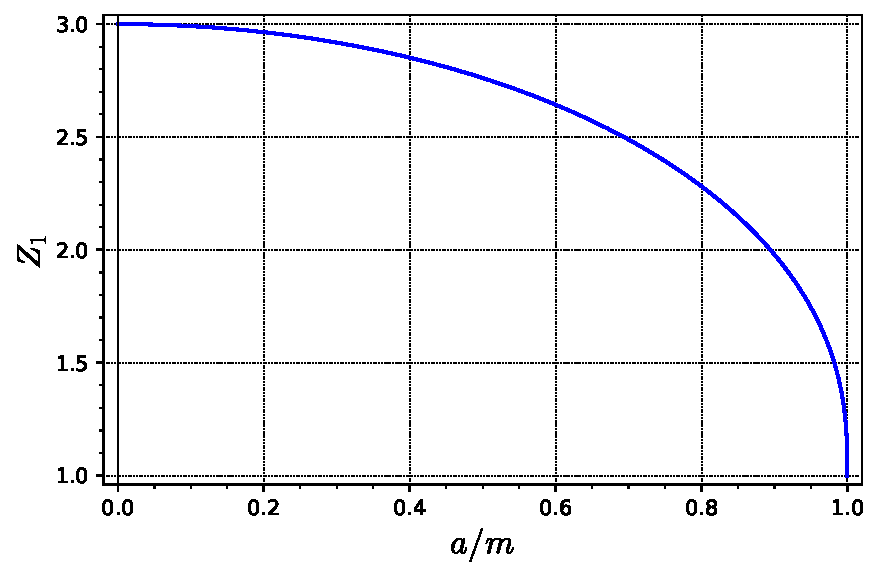
\includegraphics[width=0.7\textwidth]{gek_Z1.pdf}}
\caption[]{\label{f:gek:Z1} \footnotesize
Function $Z_1$, as defined by Eq.~(\ref{e:gek:Z1}).
\textsl{[Figure generated by the notebook \ref{s:sam:Kerr_circular_orbits}]}
}
\end{figure}
When $Z_1$ takes the value (\ref{e:gek:Z1}), the double root of $T(x)$ is
$x_0 = \pm {2a}/(3-Z_1)$, where the $\pm$ is the opposite of the $\mp$
in the definition (\ref{e:gek:def_P_T}) of $T(x)$, and therefore indicates
which family of  circular orbits, among $(\veps_+,\ell_+)$ or $(\veps_-,\ell_-)$,
is considered. We have then
\[
    S(x) = \sqrt{2(3-Z_1)} \, x \mp \frac{2\sqrt{2} \bar{a}}{\sqrt{3 - Z_1}} .
\]
When $\bar{a}\to 0$, the ratio $\bar{a}/\sqrt{3 - Z_1}$ is of the undetermined
type ``$0/0$''. We can rearrange it by noticing the identity
${8 \bar{a}^2}/(3 - Z_1) = Z_1^2 + 3 \bar{a}^2$, which is a direct consequence of
Eq.~(\ref{e:gek:cubic_Z1}). We then write
\[
     S(x) = \sqrt{2(3-Z_1)} \, x \mp Z_2,\quad\mbox{with}\quad
    Z_2 := \sqrt{Z_1^2  + 3 \bar{a}^2} .
\]
The solutions of $P(x)=0$ are obtained by solving the two quadratic equations
[cf. Eq.~ (\ref{e:gek:P_zero_S})]
\begin{subequations}
\begin{align}
& x^2 - \sqrt{2(3-Z_1)}\, x - Z_1 \pm Z_2 = 0 \label{e:gek:eq_x_Z1Z2_1} \\
& x^2 + \sqrt{2(3-Z_1)}\, x - Z_1 \mp Z_2 = 0 .  \label{e:gek:eq_x_Z1Z2_2}
\end{align}
\end{subequations}
Moreover, physically acceptable solutions must obey $x>0$ (recall that
$x := \sqrt{r_0/m}$). The discriminant of (\ref{e:gek:eq_x_Z1Z2_1}) is
$\Delta = 2(3+Z_1\mp Z_2)$. It is non-negative only when $\mp = +$, i.e.
for orbits in the $(\eps_-,\ell_-)$ family. The positive solution of (\ref{e:gek:eq_x_Z1Z2_1})
is then
\[
    x_- = \frac{1}{\sqrt{2}} \left( \sqrt{3 + Z_1 + 2 Z_2} + \sqrt{3- Z_1} \right) .
\]
On the other side, the discriminant of (\ref{e:gek:eq_x_Z1Z2_2})
is $\Delta = 2(3+Z_1 \pm 2 Z_2)$. It is non-negative only when $\pm = +$, i.e.
for orbits in the $(\eps_+,\ell_+)$ family. The positive solution of (\ref{e:gek:eq_x_Z1Z2_2})
is then
\[
    x_+ = \frac{1}{\sqrt{2}} \left( \sqrt{3 + Z_1 + 2 Z_2} - \sqrt{3- Z_1} \right) .
\]
We conclude that the quartic polynomial $P(x)$ has a single positive root, which
is
\[
    x_\pm = \frac{1}{\sqrt{2}}\left( \sqrt{3 + Z_1 + 2 Z_2} \mp \sqrt{3- Z_1} \right) .
\]
Going back to $r_0 = m x^2$, we get the single solution of $\mathcal{V}''(r_0) = 0$
on $(0, +\infty)$:
\begin{align}
 & \encadre{r_{\rm ISCO}^\pm = m \left[ 3 + Z_2 \mp \sqrt{(3 - Z_1)(3 + Z_1 + 2 Z_2)} \right] } ,
    \label{e:gek:r_ISCO} \\
&  Z_1 := 1 + \sqrt[3]{1 - \bar{a}^2} \left( \sqrt[3]{1 + \bar{a}} + \sqrt[3]{1 - \bar{a}} \right) ; \qquad
  Z_2 := \sqrt{Z_1^2  + 3 \bar{a}^2} ; \qquad \bar{a} := a/m .\nonumber
\end{align}
where $\pm$ indicates which family among $(\veps_+,\ell_+)$ and $(\veps_-,\ell_-)$ is
considered and \emph{ISCO} stands for \defin{innermost stable circular orbit}\index{stable!circular orbit}\index{innermost!stable circular orbit}\index{circular!orbit!innermost stable --}.
Indeed, $r_{\rm ISCO}^\pm $ being the unique zero of $r_0^2 - 6 m r_0 \pm 8 a \sqrt{m r_0} - 3 a^2$,
(\ref{e:gek:circ_stability_crit}) is equivalent to
\begin{greybox}
\be
\mbox{A circular orbit of radius $r_0$ is radially stable} \quad \iff \quad r_0 > r_{\rm ISCO}^\pm .
\ee
\end{greybox}
Note that $r_{\rm ISCO}^\pm  / m$ is a function of $\bar{a} := a/m$ only; this
function is depicted in Fig.~\ref{f:gek:circ_orb_isco}. We notice immediately
from it that
\be
    r_{\rm ph}^* < r_{\rm ISCO}^+
\ee
and conclude that all the inner circular orbits are unstable.
We also see on Fig.~\ref{f:gek:circ_orb_isco} that in the limit $a=0$,
$r_{\rm ISCO}^+ = r_{\rm ISCO}^- = 6 m$, i.e. we recover the Schwarzschild ISCO
discussed in Sec.~\ref{s:ges:circular_orbits}.

\begin{remark}
The ISCO is also called \defin{marginally stable circular orbit}\index{marginally!stable circular orbit} by some authors (e.g. \cite{BardePT72}), $r_{\rm ISCO}$ is then denoted by $r_{\rm ms}$.
\end{remark}

\begin{example}
For $a = 0.9\, m$, Eq.~(\ref{e:gek:r_ISCO}) yields $r_{\rm ISCO}^+ = 2.32088\, m$. Accordingly,
the prograde circular orbit at $r_0 = 3\, m$ is stable, while that at $r_0 = 2 m$ is unstable,
in agreement with the plot of $\mathcal{V}(r)$ in Fig.~\ref{f:gek:V_stability}.
\end{example}

\begin{figure}
\centerline{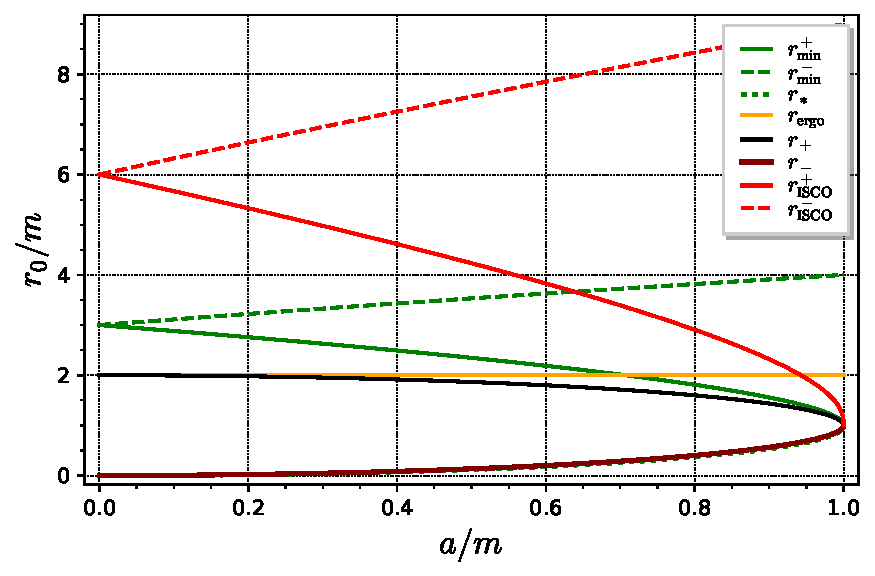
\includegraphics[width=0.8\textwidth]{gek_circ_orb_isco.pdf}}
\caption[]{\label{f:gek:circ_orb_isco} \footnotesize
Various critical radii for circular orbits as functions of the Kerr spin parameter $a$.
The red curves correspond to the innermost stable circular orbit $r_{\rm ISCO}^\pm$ [Eq.~(\ref{e:gek:r_ISCO})], the light brown ones to the marginally bound circular orbit
$r_{\rm mb}^\pm$ [Eq.~(\ref{e:gek:r_mb_circ})],
while the other curves are the same as in Fig.~\ref{f:gek:circ_orb_lim}.
\textsl{[Figure generated by the notebook \ref{s:sam:Kerr_circular_orbits}]}
}
\end{figure}

An interesting property of the ISCO is that it corresponds to extrema of
$\veps_\pm(r_0)$ and $\ell_\pm(r_0)$:
\begin{greybox} \label{p:gek:ISCO_extremum_eps_ell}
Among all prograde outer circular orbits, the ISCO is that for which
the functions $\veps_+(r_0)$ and $\ell_+(r_0)$ are minimal.
Similarly, among all retrograde outer circular orbits, the ISCO is that for
which the function $\veps_-(r_0)$ is minimal and the function $\ell_-(r_0)$
is maximal.
\end{greybox}
\begin{proof}
In what precedes, we have considered $\mathcal{V}$, defined by
Eq.~(\ref{e:gek:def_V_time_equat}), as a function of $r$ only. Let us consider
it instead as a function of $(r, \veps, \ell)$: $\mathcal{V} = \mathcal{V}(r, \veps, \ell)$.
What we have denoted by
$\mathcal{V}'(r)$ is then $\dert{\mathcal{V}}{r}$ and
Eqs.~(\ref{e:gek:circ_V_zero}) and (\ref{e:gek:circ_derV_zero}) can be rewritten
as
\begin{subequations}
\begin{align}
& \mathcal{V}\left(r_0,\; \veps_\pm(r_0),\; \ell_\pm(r_0)\right) = 0 \label{e:gek:circ_V_zero_r0} \\
& \der{\mathcal{V}}{r} \left(r_0,\; \veps_\pm(r_0),\; \ell_\pm(r_0)\right) = 0 .
    \label{e:gek:circ_derV_zero_r0}
\end{align}
\end{subequations}
These equations are valid for any circular orbit, i.e. any value of $r_0$.
Let us take the derivative of Eq.~(\ref{e:gek:circ_V_zero_r0}) with respect to $r_0$.
Using the chain rule, we get
\[
    \underbrace{\left. \der{\mathcal{V}}{r} \right| _0}_{=0}
    + \left. \der{\mathcal{V}}{\eps} \right| _0  \veps_\pm'(r_0)
    + \left. \der{\mathcal{V}}{\ell} \right| _0  \ell_\pm'(r_0) = 0 ,
\]
where $| _0$ means that the quantity is evaluated at $(r,\veps,\ell)=\left(r_0,\; \veps_\pm(r_0),\; \ell_\pm(r_0)\right)$ and the vanishing of the first term results from Eq.~(\ref{e:gek:circ_derV_zero_r0}).
Similarly, deriving Eq.~(\ref{e:gek:circ_derV_zero_r0}) with respect to $r_0$ yields
\[
    \left. \frac{\partial^2\mathcal{V}}{\partial r^2} \right| _0
    + \left. \frac{\partial^2\mathcal{V}}{\partial\eps\partial r} \right| _0  \veps_\pm'(r_0)
    + \left. \frac{\partial^2\mathcal{V}}{\partial\ell\partial r} \right| _0  \ell_\pm'(r_0)
    = 0 .
\]
Now, at the ISCO, one has precisely ${\partial^2\mathcal{V}}/{\partial r^2} |_0 = 0$
($\mathcal{V}''(r_0) = 0$ in the preceding notations). Hence, at the ISCO, the following
two equations must hold:
\be \label{e:gek:system_epsp_ellp}
    \left\{\begin{array}{l}
       \left. \der{\mathcal{V}}{\eps} \right| _0 \;  \veps_\pm'(r_0)
    + \left. \der{\mathcal{V}}{\ell} \right| _0 \;  \ell_\pm'(r_0) = 0 \\
    \left. \frac{\partial^2\mathcal{V}}{\partial\eps\partial r} \right| _0 \;  \veps_\pm'(r_0)
    + \left. \frac{\partial^2\mathcal{V}}{\partial\ell\partial r} \right| _0 \;  \ell_\pm'(r_0) = 0
    \end{array} \right.
\ee
This constitutes a linear homogeneous system for the two
unknowns $\left(\veps_\pm'(r_0),\; \ell_\pm'(r_0)\right)$.
Since there are no obvious reason for its determinant to vanish, we deduce that
the only solution is $\left(\veps_\pm'(r_0),\; \ell_\pm'(r_0)\right) = (0, 0)$.
Hence the ISCO realizes an extremum of both $\veps_\pm(r_0)$ and $\ell_\pm(r_0)$.
A quick look at Figs.~\ref{f:gek:eps_circ_orb} and \ref{f:gek:ell_circ_orb},
especially their bottom panels, enables us to conclude that the extremum is
a minimum for $\veps_\pm(r_0)$ and $\ell_+(r_0)$ and a maximum for $\ell_-(r_0)$.
\end{proof}

Because it is an extremum of both $\veps(r_0)$ and $\ell(r_0)$,
the ISCO is located at the cusp in the
$(\ell,\veps)$ curves shown in Fig.~\ref{f:gek:ell_eps_circ_orb}.

\subsubsection{Summary}

\begin{greybox}
Equatorial circular timelike orbits exist only in the region $r>0$ of Kerr spacetime.
They are all stable with respect to perturbations away from the equatorial plane.
They are of three kinds:
\begin{enumerate}
\item The \emph{prograde outer circular orbits}: they are located outside
the black hole event horizon (i.e. in region $\M_{\rm I}$), having a Boyer-Lindquist radius $r_0$ ranging
from  $r_{\rm ph}^+ = 4 m \cos^2[\arccos(-a/m)/3]$
[Eq.~(\ref{e:gek:def_r_min_pm})] to $+\infty$;
the minimal radius
$r_{\rm ph}^+$ decreases with $a$ monotonically from $3m$ ($a=0$) to $m$ ($a=m$).
These orbits are radially unstable for
$r_{\rm ph}^+ < r_0 \leq r_{\rm ISCO}^+$ and stable for $r_0 > r_{\rm ISCO}^+$,
where $r_{\rm ISCO}^+$ is given by Eq.~(\ref{e:gek:r_ISCO}),
decreasing monotonically from $6m$ ($a=0$) to $m$ ($a=m$).
Their specific conserved energy and angular momentum
are $\veps = \veps_+(r_0) >  0$ and $\ell = \ell_+(r_0) > 0$, with
$\veps_+(r_0)$ given by Eq.~(\ref{e:gek:veps_circ}) and $\ell_+(r_0)$ by
Eq.~(\ref{e:gek:ell_circ}), both being plotted as the solid
curves in the region $r_0 \geq m$ of Figs.~\ref{f:gek:eps_circ_orb} and \ref{f:gek:ell_circ_orb}.
The functions $\veps_+(r_0)$ and $\ell_+(r_0)$ are minimal at the ISCO.
\item The \emph{retrograde outer circular orbits}: they are located outside
the black hole event horizon (i.e. in region $\M_{\rm I}$), having a Boyer-Lindquist radius $r_0$ ranging
from $r_{\rm ph}^- = 4 m \cos^2[\arccos(a/m)/3]$
[Eq.~(\ref{e:gek:def_r_min_pm})] to $+\infty$; the minimal radius
$r_{\rm ph}^-$ increases with $a$ monotonically from $3m$ ($a=0$) to $4m$ ($a=m$).
These orbits are radially unstable for
$r_{\rm ph}^- < r_0 \leq r_{\rm ISCO}^-$ and stable for $r_0 > r_{\rm ISCO}^-$,
where $r_{\rm ISCO}^-$ is given by Eq.~(\ref{e:gek:r_ISCO}),
increasing monotonically from $6m$ ($a=0$) to $9m$ ($a=m$).
Their specific conserved energy and angular momentum
are $\veps = \veps_-(r_0) > 0$ and $\ell = \ell_-(r_0) < 0$, with
$\veps_-(r_0)$ given by Eq.~(\ref{e:gek:veps_circ}) and $\ell_-(r_0)$ by
Eq.~(\ref{e:gek:ell_circ}), both being plotted as the dashed
curves in Figs.~\ref{f:gek:eps_circ_orb} and \ref{f:gek:ell_circ_orb}.
The functions $\veps_-(r_0)$ and $|\ell_-(r_0)|$ are minimal at the ISCO.
\item The \emph{inner circular orbits}: they are located inside the inner horizon
(in the part $r>0$ of region $\M_{\rm III}$),
having a Boyer-Lindquist radius $r_0$ ranging
from $0$ (the ring singularity) to
$r_{\rm ph}^* = 4 m \cos^2[\arccos(-a/m)/3 + 4\pi/3]$
[Eq.~(\ref{e:gek:def_r_star})];
the maximal radius $r_{\rm ph}^*$ increases with $a$ monotonically from $0$ ($a=0$) to $m$ ($a=m$).
These orbits are all radially unstable. Their specific conserved energy and angular momentum
are $\veps = \veps_+(r_0)$ and $\ell = \ell_+(r_0)$, with
$\veps_+(r_0)$ given by Eq.~(\ref{e:gek:veps_circ}) and $\ell_+(r_0)$ by
Eq.~(\ref{e:gek:ell_circ}), both being plotted as the solid
curves in the region $r_0 \leq m$ of Figs.~\ref{f:gek:eps_circ_orb} and \ref{f:gek:ell_circ_orb}.
\end{enumerate}
In particular, there are no equatorial circular orbits in region $\M_{\rm II}$ of Kerr spacetime.
\end{greybox}


\begin{figure}
\begin{center}
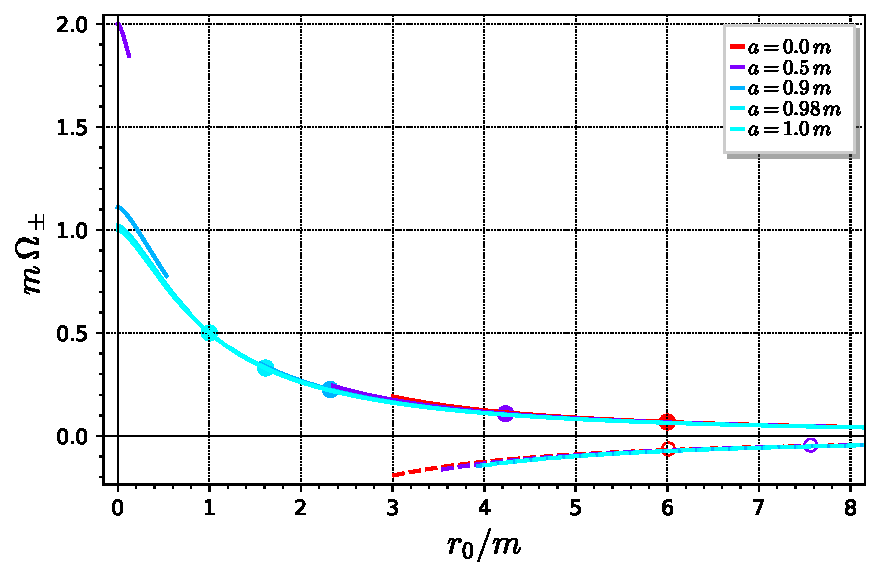
\includegraphics[width=0.65\textwidth]{gek_omega_circ_orb.pdf}\\
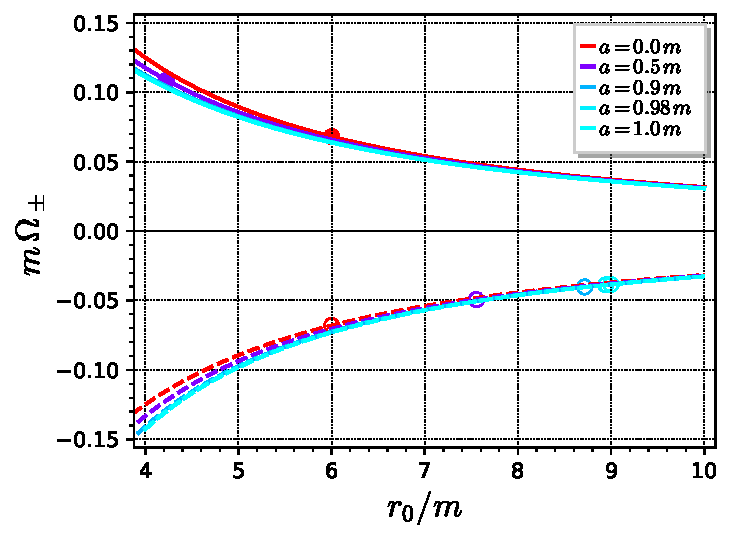
\includegraphics[width=0.65\textwidth]{gek_omega_circ_orb_zoom.pdf}
\end{center}
\caption[]{\label{f:gek:omega_circ_orb} \footnotesize
Angular velocity $\Omega:=\D\ph/\D t=\Omega_+$ (solid curves) or $\Omega=\Omega_-$
(dashed curves) along circular timelike
orbits in the equatorial plane, as a function of the orbital radius $r_0$
[Eq.~(\ref{e:gek:Omega_circ})], for selected values of the Kerr spin parameter $a$.
Dots on $\Omega_+$ curves and open circles on $\Omega_-$ ones mark the ISCO: all
configurations on the left of these points are unstable.
The bottom panel is a zoom on the region $4\,m \leq r_0 \leq 10\,m$.
\textsl{[Figure generated by the notebook \ref{s:sam:Kerr_circular_orbits}]}
}
\end{figure}

\subsection{4-velocity and angular velocities} \label{s:gek:circ_velocities}

The orbiting angular velocity as seen by an asymptotic inertial observer is
$\Omega := \D\ph/\D t |_\Li$ (cf. Sec.~\ref{s:ges:circular_orbits} for the
Schwarzschild case and Sec.~\ref{s:ker:station_obs} for the extension to Kerr
spacetime).
We evaluate it by combining Eqs.~(\ref{e:gek:timel_dtdtau}) and (\ref{e:gek:timel_dphdtau}):
\[
    \Omega = \frac{\D\ph}{\D\tau} \times \frac{\D\tau}{\D t}
        = \frac{ \left( 1 - \frac{2m}{r_0} \right) \ell
    + \frac{2 am \veps}{r_0} }{(r_0^2 + a^2) \veps + \frac{2 a m}{r_0} (a\veps - \ell)} .
\]
Using $\tilde{\ell} = \ell - a\veps$ [Eq.~(\ref{e:gek:def_tilde_l})] instead of $\ell$, we
get
\[
    \Omega = \frac{(r_0 - 2m) \tilde{\ell} + a r_0 \veps}{r_0(r_0^2 + a^2) \veps
    - 2 a m \tilde{\ell}} .
\]
Substituting $\veps$ and $\tilde{\ell}$ by the actual values $\veps_\pm$
and $\tilde{\ell}_\pm$ taken on a circular orbit [Eqs.~(\ref{e:gek:veps_circ})
and (\ref{e:gek:tell_circ})], we obtain, after simplification,
\be \label{e:gek:Omega_circ}
    \encadre{\Omega_\pm = \pm \frac{\sqrt{m}}{r_0^{3/2} \pm a \sqrt{m}} } ,
\ee
where $\Omega_+$ is the value of $\Omega$ for prograde outer circular orbits
and inner circular orbits and $\Omega_-$ is the value for retrograde
outer circular orbits. $\Omega_+$ and $\Omega_-$ are drawn in term of $r_0$
in Fig.~\ref{f:gek:omega_circ_orb}. Note that for $r_0 \gtrsim 7\, m$,
the effect of spin parameter $a$ on $\Omega_\pm$ is hardly perceptible.

\begin{remark}
For $a\to 0$, Eq.~(\ref{e:gek:Omega_circ}) reduces to Eq.~(\ref{e:ges:Omega_m_r}), as it should.
\end{remark}

From the very definition (\ref{e:gek:def_circular_orbit}) of a circular orbit
in the equatorial plane, the 4-velocity $\w{u}$ along such an orbit
obeys $u^r = \D r/\D\tau = 0$ and $u^\th = \D\th/\D\tau = 0$. Since morever
$\Omega = \D\ph/\D t = u^\ph / u^t$, $\wpar_t = \w{\xi}$ and $\wpar_\ph = \w{\eta}$,
we can write the 4-velocity as
\be \label{e:gek:4vel_circ_orb}
    \encadre{ \w{u} = u^t \left( \w{\xi} + \Omega_\pm \w{\eta} \right) } .
\ee
The component $u^t = \D t / \D\tau$ is given by Eq.~(\ref{e:gek:timel_dtdtau}).
Substituting in it Eq.~(\ref{e:gek:veps_circ}) for $\veps$
and Eq.~(\ref{e:gek:tell_circ}) for $\tilde{\ell} := \ell - a \veps$, we
get, after simplification:
\be \label{e:gek:ut_circ_orb}
    u^t = \frac{r_0 \pm a \sqrt{m/r_0}}{\sqrt{r_0^2 - 3m r_0 \pm 2 a \sqrt{m r_0}}} .
\ee

Equation~(\ref{e:gek:4vel_circ_orb}) shows that the 4-velocity is a linear
combination of the two Killing vectors $\w{\xi}$ and $\w{\eta}$ with
coefficients that are constant along the worldline $\Li$. An observer on
a circular orbit in the equatorial plane is thus a
\emph{stationary observer}\index{stationary!observer!in Kerr spacetime}\index{observer!stationary --} as defined in Sec.~\ref{s:ker:station_obs}
[compare Eq.~(\ref{e:ker:4vel_stat_obs_omega})]. He does not notice any change in the spacetime
geometry. We shall call him a \defin{circular geodesic observer}\index{circular!geodesic!observer}\index{observer!circular geodesic --}.
Contrary to the families of stationary observers considered in Sec.~\ref{s:ker:observers},
a circular geodesic observer is in free fall: by construction, his worldline is a geodesic, so that
his 4-acceleration is zero.

The orbital velocity measured by the circular geodesic observer himself is
$\Omega_{\mathscr{P}} = \D\ph / \D\tau = \D\ph / \D t \times \D t / \D \tau = u^t \Omega$.
Using the values (\ref{e:gek:Omega_circ}) and (\ref{e:gek:ut_circ_orb}), we get
\be
    \Omega_{\mathscr{P}}^\pm = \pm \frac{\sqrt{m} \pm a m r_0^{-3/2}}{(\sqrt{r_0} \pm a\sqrt{m}/r_0)\sqrt{r_0^2 - 3m r_0 \pm 2 a \sqrt{m r_0}}} .
\ee
The orbital period measured by the circular geodesic observer is
$T_{\mathscr{P}}^\pm = 2\pi / |\Omega_{\mathscr{P}}^\pm |$.


\begin{figure}
\centerline{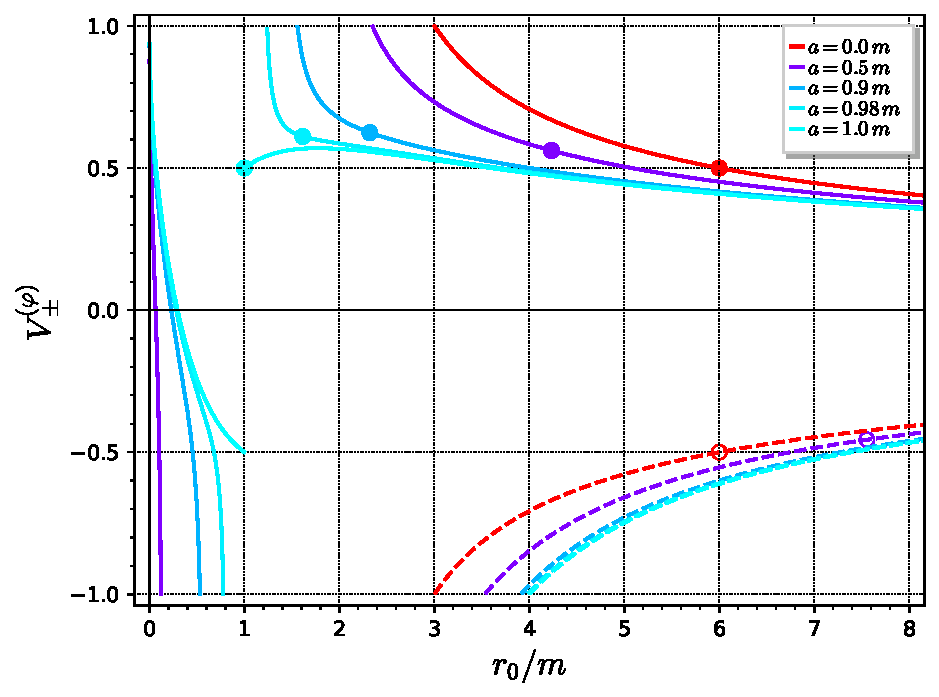
\includegraphics[width=0.7\textwidth]{gek_v_zamo_circ_orb.pdf}}
\caption[]{\label{f:gek:v_zamo_circ_orb} \footnotesize
Component $V^{(\ph)}_+$  (solid curves) or $V^{(\ph)}_-$
(dashed curves) of the velocity $\w{V} = V^{(\ph)}_\pm \, \w{e}_{(\ph)}$
of a particle moving along a circular
orbit as measured by the ZAMO [Eq.~(\ref{e:gek:v_ZAMO_circ_orb})]
for selected values of the Kerr spin parameter $a$.
Dots on $V^{(\ph)}_+$  curves and open circles on $V^{(\ph)}_-$  ones mark the ISCO: all
configurations on the left of these points are unstable.
\textsl{[Figure generated by the notebook \ref{s:sam:Kerr_circular_orbits}]}
}
\end{figure}

It is instructive to evaluate the velocity $\w{V}$ of a particle $\mathscr{P}$
on a circular orbit as measured by a zero-angular momentum observer (ZAMO)
(cf. Sec.~\ref{s:ker:ZAMO}).
Let us first note that all circular orbits are within the domain of ZAMOs,
$\M_{\rm ZAMO} = \M_{\rm I} \cup (\M_{\rm III}\setminus \mathscr{T})$
[Eq.~(\ref{e:ker:ZAMO_domain})]. Indeed, the outer circular orbits are in $\M_{\rm I}$
and the inner ones are in the part $r>0$ of $\M_{\rm III}$, while the
Carter time machine $\mathscr{T}$ is located in the part $r<0$ (cf. Sec.~\ref{s:ker:time_machine}).
Let us then rewrite
formula (\ref{e:gek:4vel_circ_orb}) for $\mathscr{P}$'s 4-velocity $\w{u}$
by expressing $\w{\xi}$ in terms of the ZAMO's 4-velocity $\w{n}$, the lapse $N$
and the shift vector $\w{\beta}$
via Eq.~(\ref{e:ker:xi_3p1_ZAMO}):
\[
    \w{u} = u^t\left( N \w{n} + \w{\beta} + \Omega_\pm \w{\eta} \right)
      = u^t \left[ N \w{n} + (\Omega_\pm - \omega)\, \w{\eta} \right]
      = N u^t \left[ \w{n} + \frac{1}{N} (\Omega_\pm - \omega) \, \w{\eta} \right],
\]
where the second equality results from
$\w{\beta} = \beta^\ph \wpar_\ph = \beta^\ph \w{\eta} = - \omega \w{\eta}$,
$\omega$ being the rotation angular velocity of the ZAMO seen from
infinity [Eq.~(\ref{e:ker:omega_ZAMO})]. Since $\w{n}\cdot\w{\eta} = 0$, the
above formula constitute the orthogonal decomposition of $\w{u}$ with
respect to the ZAMO's 4-velocity $\w{n}$, which we can compare to the generic
formula (\ref{e:fra:u_Gamma_V}) and thereby conclude that
the velocity of $\mathscr{P}$ with respect to the ZAMO is
\be
    \w{V} = \frac{1}{N} (\Omega_\pm - \omega)\,  \w{\eta}
\ee
and the Lorentz factor of $\mathscr{P}$ with respect to the ZAMO is
\be
    \Gamma = ( 1 - \w{V}\cdot\w{V})^{-1/2} = N u^t .
\ee
Let us expand $\w{V}$ on the ZAMO's orthonormal fame $(\w{e}_{(\alpha)})$
[Eq.~(\ref{e:ker:def_ZAMO_frame})]. Given relation (\ref{e:ker:ZAMO_frame_ph})
between $\w{\eta} = \wpar_\ph$ and $\w{e}_{(\ph)}$ we get, after
substituting Eq.~(\ref{e:ker:lapse_ZAMO}) (with $\th=\pi/2$) for $N$:
\[
  \w{V} = \frac{r_0^2 + a^2 + 2a^2 m/r_0}{\sqrt{r_0^2 - 2 m r_0 + a^2}}
      (\Omega_\pm - \omega)\, \w{e}_{(\ph)} .
\]
Finally, let us substitute Eq.~(\ref{e:gek:Omega_circ}) for $\Omega_\pm$
and Eq.~(\ref{e:ker:omega_ZAMO}) (with $\th=\pi/2$) for $\omega$. We obtain,
after simplification:
\be \label{e:gek:v_ZAMO_circ_orb}
    \encadre{ \w{V} = V^{(\ph)}_\pm  \, \w{e}_{(\ph)}}
    \quad \mbox{with} \quad
    \encadre{V^{(\ph)}_\pm = \pm \frac{\sqrt{m} \left( r_0^2 \mp 2a \sqrt{m r_0} + a^2\right)}%
    {(r_0^{3/2} \pm a \sqrt{m})\sqrt{r_0^2 - 2 m r_0 + a^2}} } .
\ee
As in all formulas of this section, the sign $\pm$ is $+$ for a prograde outer circular orbit
or an inner circular orbit and $-$ for a retrograde outer circular orbit.
The velocity $V^{(\ph)}_\pm$ is depicted in Fig.~\ref{f:gek:v_zamo_circ_orb}.
We note that, except for $a=m$,
\be
    \lim_{r_0 \to 0} V^{(\ph)}_+ = 1, \quad \lim_{r_0 \to r_{\rm ph}^*} V^{(\ph)}_+ = - 1,
    \quad \lim_{r_0 \to r_{\rm ph}^+} V^{(\ph)}_+ = 1,
    \quad \lim_{r_0 \to r_{\rm ph}^-} V^{(\ph)}_- = -1 .
\ee
Since $\w{e}_{(\ph)}$ is a unit vector, this means that
\begin{itemize}
\item the inner orbits rotate close to the speed of light with respect
to the ZAMO near the ring singularity ($r_0\to 0$) and near the outer boundary
of their domain of existence ($r_0 \to r_{\rm ph}^*$), this motion being
in the prograde (resp. retrograde) direction in the first (resp. second) case;
\item the outer orbits rotate at the speed of light with respect
to the ZAMO near the minimal radius of their domain of existence
($r_0\to r_{\rm ph}^\pm$).
\end{itemize}
Given that the velocity of a massive particle with respect to any observer
cannot be larger than the speed of light, this provides a physical explanation
for the boundaries of the domains of existence of circular orbits obtained
in Sec.~\ref{s:gek:existence_circ_orb}. We shall see in Sec.~\ref{s:gik:spherical_orbits} that
these boundaries correspond to photon circular orbits.
This also provides a physical explanation why the specific conserved energy
$\veps$ and the specific conserved angular momentum $\ell$ diverge
at these boundaries, as observed in Figs.~\ref{f:gek:eps_circ_orb} and \ref{f:gek:ell_circ_orb}:
$\veps := E/\mu$ and $\ell := L/\mu$ must tend to $\pm\infty$ when the particle's mass $\mu$ tends to
0 (the photon limit).

The particular case $a=m$ will be discussed in Sec.~??.


\subsection{Marginally bound circular orbit}

We see on Fig.~\ref{f:gek:eps_circ_orb} that for $a \neq m$ and $r_0$ lower than a critical
value, $r_{\rm mb}^+$ say, the prograde outer circular orbits have $\veps > 1$
(cf. the grey horizontal line in Fig.~\ref{f:gek:eps_circ_orb}), which is equivalent to
$E>\mu$; they are thus unbound (cf. Sec.~\ref{s:gek:bound_geod}). Conversely, all
orbits with $r_0 > r_{\rm mb}^+$ are bound.
Similarly, but this time of all values of $a\leq m$,
the retrograde outer circular orbits are bound iff $r_0$ is larger than
a critical value, $r_{\rm mb}^-$ say. The orbit at $r_0 = r_{\rm mb}^\pm$ is
called the \defin{marginally bound circular orbit}\index{marginally!bound!circular orbit}\index{circular!orbit!marginally bound --}.

We note from Fig.~\ref{f:gek:eps_circ_orb} that
\be
    r_{\rm ph}^\pm < r_{\rm mb}^\pm < r_{\rm ISCO}^\pm .
\ee
Accordingly, all unbound orbits are unstable.

To evaluate $r_{\rm mb}^\pm$, let us solve the equation $\veps_\pm(r_0) = 1$ for $r_0$.
Using expression (\ref{e:gek:veps_circ}) for $\veps_\pm(r_0)$, taking the square
and simplifying, we get
\[
    r_0^2 - 4 m r_0 \pm 4 a \sqrt{m r_0} - a^2 = 0 ,
\]
which we can write
\[
    r_0^2 = (2\sqrt{mr_0} \mp a)^2  .
\]
Since we are looking for solutions $r_0 \geq r_+ = m + \sqrt{m^2 - a^2}$, we have
$2\sqrt{m r_0} \mp a > 0$, so that we can reduce the above equation to
$r_0 = 2\sqrt{m r_0} \mp a$. Introducing $x := \sqrt{r_0/m}$, we end up solving
the quadratic equation $x^2 - 2 x \pm a/m = 0$.
The only solution $x \geq 1$, which is implied by $r_0 \geq r_+$, is
$x = 1 + \sqrt{1 \mp a/m}$. This yields
\be \label{e:gek:r_mb_circ}
    \encadre{ r_{\rm mb}^\pm = 2 m \mp a + 2 \sqrt{m(m\mp a)} } .
\ee
$r_{\rm mb}^\pm$ is plotted as a function of $a$ in Fig.~\ref{f:gek:circ_orb_isco}.

\subsection{Circular orbits in the ergoregion}

We see in Fig.~\ref{f:gek:circ_orb_isco} that for $a$ sufficiently large,
prograde outer circular orbits can exist in the outer ergoregion\index{outer!ergoregion}\index{ergoregion!outer --} $\mathscr{G}^+$
(cf. Sec.~\ref{s:ker:ergoregion}), while no retrograde outer circular orbits
can exist there.
In the equatorial plane, the coordinate $r$
of the external boundary of $\mathscr{G}^+$
(the outer ergosphere\index{outer!ergosphere}\index{ergosphere!outer --}) is
simply $r_{\E^+}(\pi/2) = 2 m$ [Eq.~(\ref{e:ker:r_ergo_p_eq})] --- the orange
horizontal line in Fig.~\ref{f:gek:circ_orb_isco}.
Thus, prograde outer circular orbits exist in the ergoregion if
$r_{\rm ph}^+ < 2 m$ and they can be stable if $r_{\rm ISCO}^+ < 2 m$.
The limiting value of $a$ for the first case is obtained by setting
$r_0 = 2 m$ in the equation governing the existence of prograde circular orbits,
namely Eq.~(\ref{e:gek:cubic_sqrt_r0}) with the $+$ sign:
$(2m)^{3/2} - 3 m \sqrt{2m} + 2 a \sqrt{m} > 0$,
from which we get immediately
\begin{greybox}
\be \label{e:gek:orb_in_ergo}
    \left( {\mbox{timelike circular orbits}\atop
     \mbox{exist in the outer ergoregion}} \right)
     \iff a > \frac{m}{\sqrt{2}} \simeq 0.707\, m .
\ee
\end{greybox}
Similarly, the limiting value of $a$ for the stability of
circular orbits in the ergoregion is obtained by setting $r_0 = 2m$ in
Eq.~(\ref{e:gek:circ_stability_crit}) with the $+$ sign:
$(2 m)^2 - 12 m^2 + 8 a m\sqrt{2} - 3 a^2 > 0$.
The right-hand side being a quadratic polynomial in $a$, we get
easily, given the constraint $a \leq m$,
\begin{greybox}
\be \label{e:gek:stable_orb_in_ergo}
    \left( {\mbox{timelike circular orbits}\atop
     \mbox{exist stably in the ergoregion}} \right)
     \iff a > \frac{2\sqrt{2}}{3} m \simeq 0.943\, m .
\ee
\end{greybox}
Both in (\ref{e:gek:orb_in_ergo}) and (\ref{e:gek:stable_orb_in_ergo}), the
orbits referred to belong to the prograde outer family.

\begin{remark}
Regarding the limit (\ref{e:gek:orb_in_ergo}), the existence is specified to
be in the \emph{outer} ergoregion, because timelike circular orbits always
exist, as soon as $a>0$, in the inner ergoregion: they are the (unstable) inner circular
orbits found in Sec.~\ref{s:gek:existence_circ_orb}. Indeed, these orbits exist
in the range $0 < r_0 < r_{\rm ph}^*$, which is entirely contained in the
inner ergoregion: the boundaries of the latter in the equatorial plane are
$r=0$ [Eq.~(\ref{e:ker:r_ergo_m_eq})] and $r=r_-$, with $r_- > r_{\rm ph}^*$.
On the contrary, in the limit (\ref{e:gek:stable_orb_in_ergo}), we have
dropped the qualifier \emph{outer} for the ergoregion, since there is no other
place where stable circular orbits can be found, the inner circular orbits
being all unstable.
\end{remark}

\begin{remark}
As discussed in Sec.~\ref{s:gek:sign_E}, negative-energy or zero-energy particles can exist in
the outer ergoregion. However, Fig.~\ref{f:gek:eps_circ_orb} shows us that none
of them can follow a circular orbit.
\end{remark}



\begin{hist}
The solutions for the circular geodesic motion in the equatorial plane
for outer prograde and outer retrograde orbits have been published for the first
time by James M. Bardeen\index{Bardeen, J.M.}, William H. Press\index{Press, W.H.} and Saul A. Teukolsky\index{Teukolsky, S.A.} in 1972 \cite{BardePT72}. In his lecture notes at the famous
1972 Les Houches School \cite{Barde73}, Bardeen says that they have been derived by Teukolsky.
In the article \cite{BardePT72}, it is mentioned that they have been derived by means of
computer algebra techniques.
\end{hist}

%%%%%%%%%%%%%%%%%%%%%%%%%%%%%%%%%%%%%%%%%%%%%%%%%%%%%%%%%%%%%%%%%%%%%%%%%%%%%%%








\section{Going further}

For an extended discussion of geodesics of Kerr spacetime, including those
that cross the various blocks of the maximal analytic extension presented in
Sec.~\ref{s:ker:max_extension}, see Chap.~4 of O'Neill textbook \cite{ONeil95}.

